\chapter{Calcualtion results and analysis}
Once all the experiment data and parameters are determined, the results 
of the calculation should be presented and analyzed. Thus, the 
accuracy, consistency, pros and cons of the virtual experiment 
platform and temperature estimation algorithm can be systematically 
analyzed.

\section{Calculation results}
In virtual experiment platform and temperature estimation algorithms, emissivity is considered as a 
function of radiation wavelength and temperature. Consequently, it varies with changes in 
temperature and radiation wavelength. This variability is advantageous for enhancing algorithm 
precision but introduces difficulties in visualizing computation results. Furthermore, 
temperature estimation algorithm doesn't directly calculate the emissivity of materials; 
instead, the algorithm optimize the parameters $k$ of the emissivity model. 
Thus, the emissivity data of each point is a function of wavelength $\lambda$ and thus
cannot be directly visualized. To address this, a simplified 
approach for visualizing emissivity is introduced, which allows for a more intuitive 
representation of emissivity without compromising the accuracy of the computational process.

\begin{equation}
    \label{eq: emi_average}
    \varepsilon_{sim} = \overline{\varepsilon(\lambda)} 
\end{equation}

Eq.\ref{eq: emi_average} presents the mathematical expression for this simplification. 
$\varepsilon_{sim}$ represents the simplified emissivity value, and $\varepsilon(\lambda)$ denotes 
the emissivity model's value at wavelength $\lambda$. In other words, in this work, the 
visualization of emissivity is derived from the average value of emissivity model data 
within the wavelength range of 500 to 1000 nanometers.


By employing the same simplification method in the generation of experimental data and 
subsequent temperature estimation algorithm, the validity of the program's verification is 
ensured. This consistency guarantees that the comparison between the data used for 
validation remains effective and reliable throughout the process.


After obtaining a standardized emissivity visualization method, it is necessary to validate the 
calculation results. For the convenience of validation, several data that cannot be 
obtained in real experiments, such as temperature and emissivity of hypothetical material 
have been saved in several files in the virtual experiment platform and used to 
check the accuracy in validation process.


\subsection{Raw experiment data from virtual experiment platform}
In order to assess the performance of the temperature estimation algorithm 
at different temperatures and facilitate visual analysis, a linear temperature 
distribution is employed during the validation process. The background 
temperature is set to 1000K, while the center point's temperature is 
set at 1900K. Details is shown in Fig.\ref{fig: t_field}. Simultaneously, the melting point of the hypothetical material 
is defined as 1600K (except black body and gray body hypothetical material). 
This approach allows for the comparison of data obtained 
from the virtual experimental platform with that from real experiments, 
while checking the accuracy of the temperature estimation algorithm in 
both solid and liquid phase of the hypothetical material.


\begin{figure}[htbp]
    \centering
    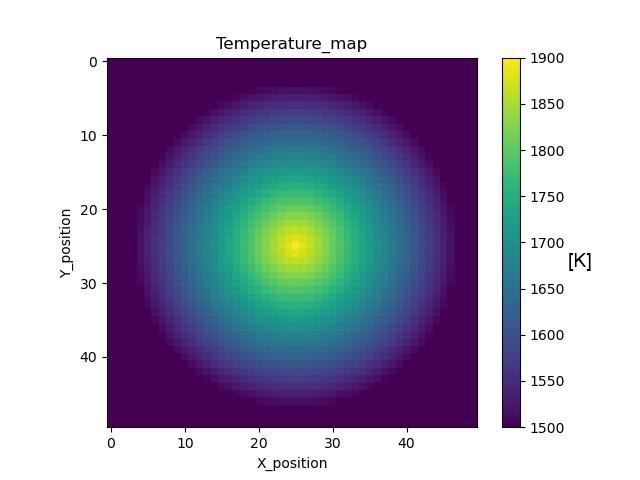
\includegraphics[width=0.8\textwidth]{figures/t_field.jpg}
    \caption{Temperature field used in validation}
    \label{fig: t_field}
\end{figure}


After obtaining a temperature field, the virtual experimental platform 
used the aforementioned 12 different emissivity models to generate 12 
different sets of experimental data. This approach simulated the radiative 
behavior of 12 hypothetical materials under identical temperature conditions 
in the virtual experiment platform.

\begin{figure}[htbp]
    \centering
    \begin{minipage}{\textwidth}
        \centering
        \begin{subfigure}{0.45\textwidth}
            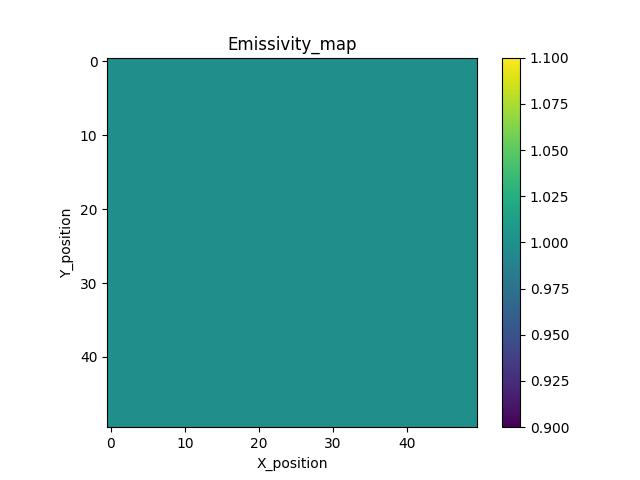
\includegraphics[width=\textwidth]{figures/raw_data/0/emi_field.jpg}
        \end{subfigure}
        \begin{subfigure}{0.45\textwidth}
            \centering
            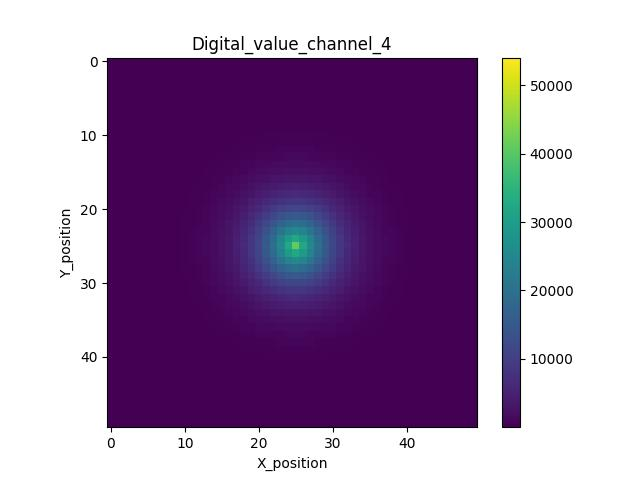
\includegraphics[width=\textwidth]{figures/raw_data/0/digital_value_channel_4.jpg}
        \end{subfigure}
        \subcaption{Black body}
        \label{fig: raw_data_0}
    \end{minipage}\\
    \begin{minipage}{\textwidth}
        \centering
        \begin{subfigure}{0.45\textwidth}
            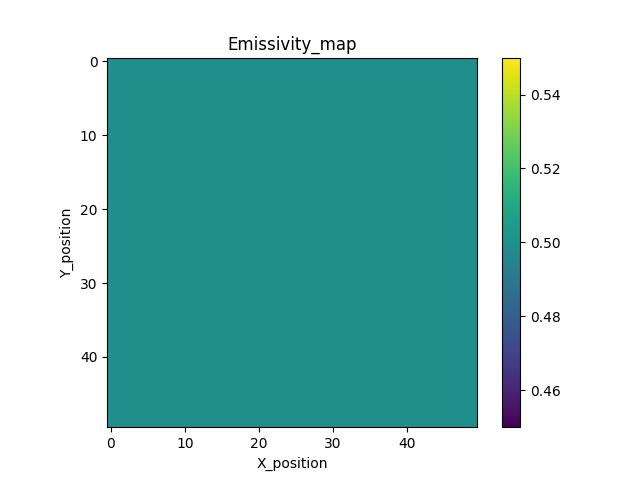
\includegraphics[width=\textwidth]{figures/raw_data/1/emi_field.jpg}
        \end{subfigure}
        \begin{subfigure}{0.45\textwidth}
            \centering
            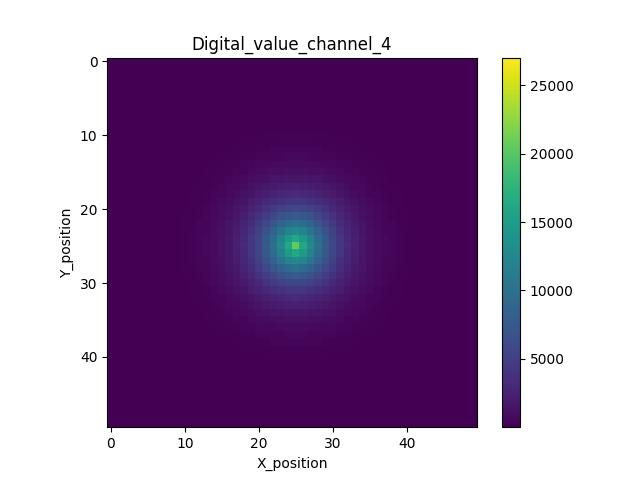
\includegraphics[width=\textwidth]{figures/raw_data/1/digital_value_channel_4.jpg}
        \end{subfigure}
        \subcaption{Gray body}
        \label{fig: raw_data_1}
    \end{minipage}\\
    \begin{minipage}{\textwidth}
        \centering
        \begin{subfigure}{0.45\textwidth}
            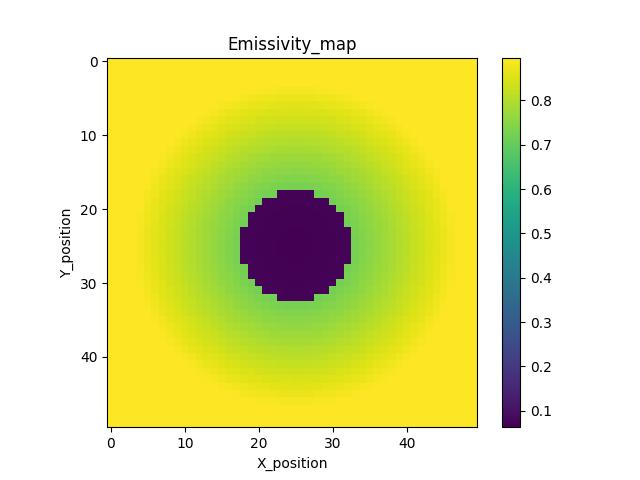
\includegraphics[width=\textwidth]{figures/raw_data/21/emi_field.jpg}
        \end{subfigure}
        \begin{subfigure}{0.45\textwidth}
            \centering
            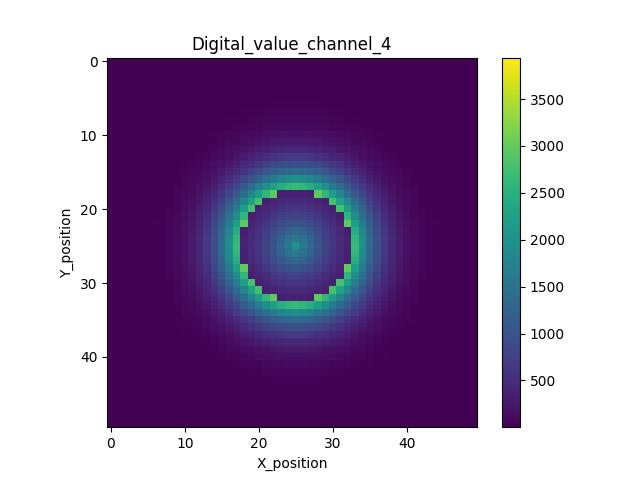
\includegraphics[width=\textwidth]{figures/raw_data/21/digital_value_channel_4.jpg}
        \end{subfigure}
        \subcaption{Model 1}
        \label{fig: raw_data_21}
    \end{minipage}\\
    \begin{minipage}{\textwidth}
        \centering
        \begin{subfigure}{0.45\textwidth}
            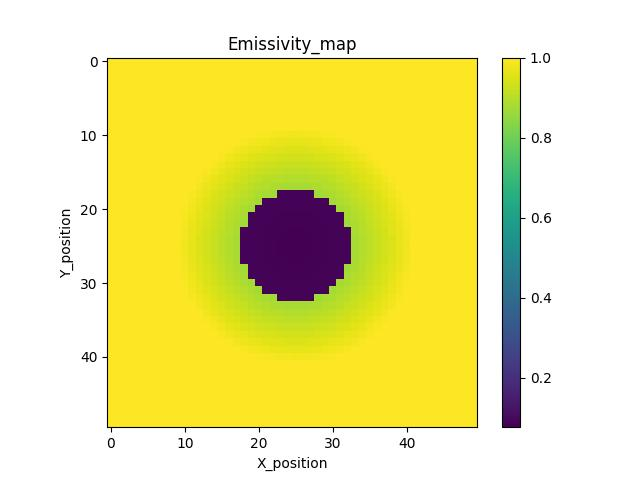
\includegraphics[width=\textwidth]{figures/raw_data/32/emi_field.jpg}
        \end{subfigure}
        \begin{subfigure}{0.45\textwidth}
            \centering
            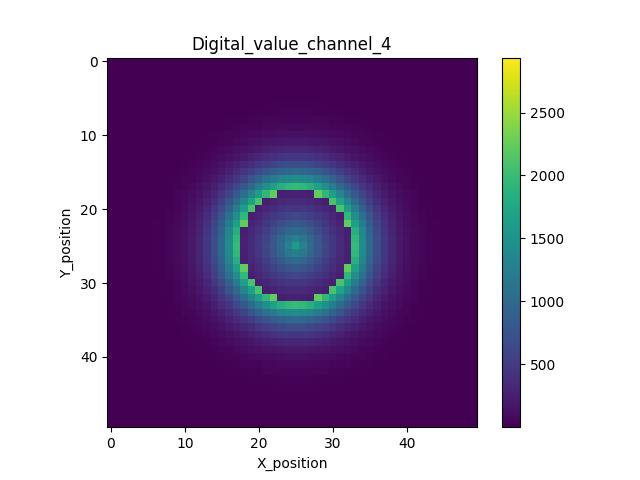
\includegraphics[width=\textwidth]{figures/raw_data/32/digital_value_channel_4.jpg}
        \end{subfigure}
        \subcaption{Model 8}
        \label{fig: raw_data_32}
    \end{minipage}
    \caption{Emissivity field and digital value of radiation intensity in channel 4 for 
    black body material(\subref{fig: raw_data_0}), gray body material(\subref{fig: raw_data_1}), 
    material based on model 1(\subref{fig: raw_data_21}) and model 8(\subref{fig: raw_data_32})}
    \label{fig: raw_data}
\end{figure}

As a result, Fig.\ref{fig: raw_data} displays the emissivity fields generated by defferent
model along with their corresponding radiation intensities. To conserve space, 
digital values of channel 4 in each experiment data were chosen as 
representatives of the intensity data.


It can be observed that in blackbody and gray body materials, emissivity is not 
dependent on the material's temperature or status. As a result, the emissivity 
field exhibits a uniform color distribution. This characteristic also leads to a 
situation in the calculation of radiation intensity, where the physical values 
received by the virtual camera show a maximum at the center point and decrease 
as the temperature decreases.


However, in more general material models, such as Model 1 and Model 8, emissivity 
undergoes a discontinuity when the material transitions from the solid state to 
the liquid state. This is due to the fact that the emissivity of liquid phase 
is smaller than that of solid phase. Consequently, the radiation intensity 
received by the virtual camera decreases at the boundary when the material 
changes from solid to a liquid. Subsequently, at the center point, the radiation 
intensity emitted by the hypothetical material increases again due to the rise in 
temperature. This phenomenon results in a bright halo appearing in the digital 
value of channel 4 in the images. The center of this 
halo exhibits a point with higher brightness level.


Indeed, the non-uniform intensity distribution caused by different emissivity 
characteristics of materials can lead to challenges for the subsequent 
temperature estimation algorithm. The intensity distribution along wavelength 
differs due to the different emissivity model of the hypothetical material. 
Consequently, in the curve fit algorithm, the most suitable emissivity model for 
the current material may change accordingly. Therefore, particular attention 
should be given to the phase transition of the hypothetical material in the 
context of temperature estimation. 


After investigating the impact of different emissivity models on material 
radiative characteristics, it is necessary to explore the relationship between 
digital values of radiation intenstiy across different channels. 
Fig.\ref{fig: channel} displays the images of a material based on Model 1 at a 
temperature of 1900K, captured using 8 different channels. In this image, 
it can be observed that the intensity received by the virtual camera increases 
with the channel number.

\begin{figure}[htbp]
    \centering
    \begin{minipage}{0.10\textwidth}
        \centering
        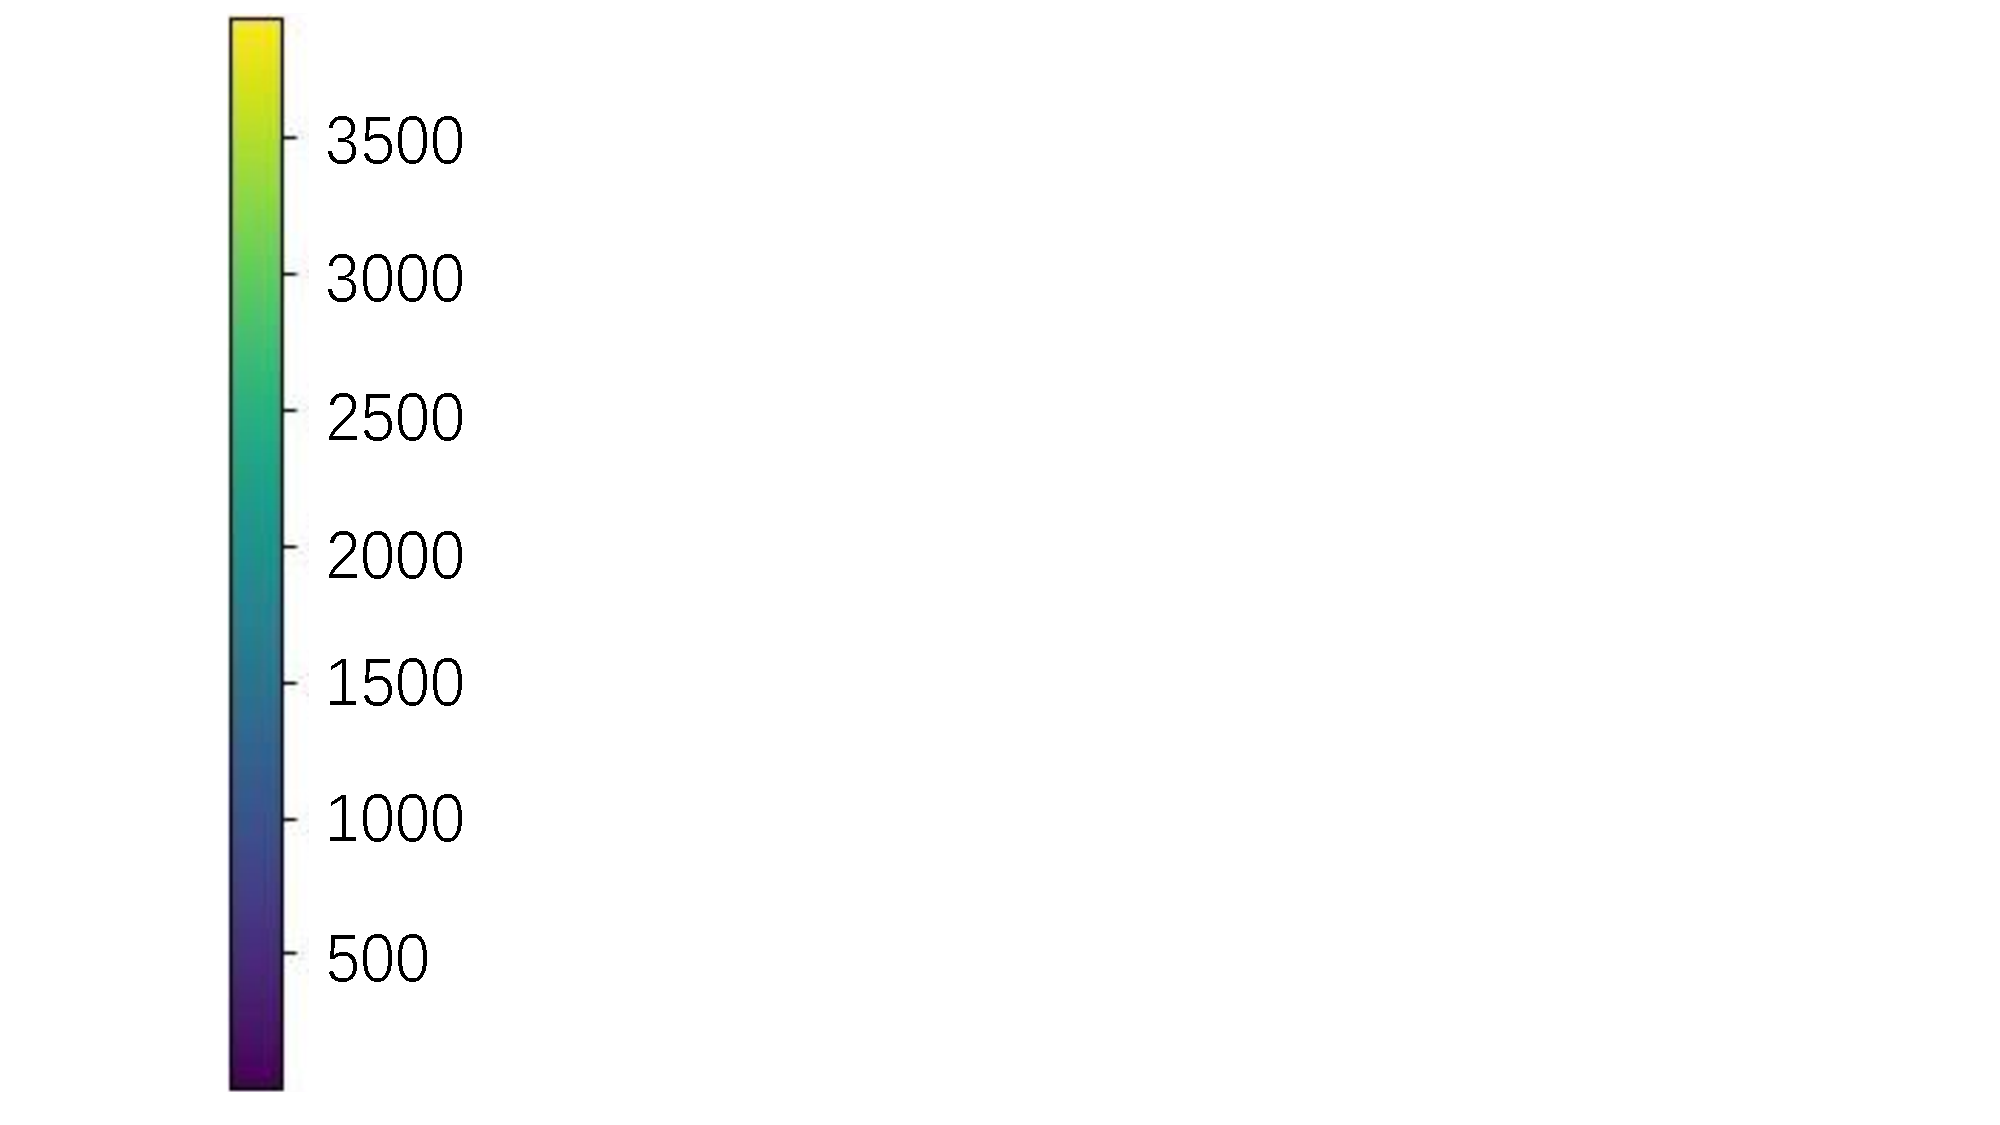
\includegraphics[width=\textwidth]{figures/raw_data/21/color_bar.pdf}
    \end{minipage}
    \begin{minipage}{0.87\textwidth}
        \centering
        \begin{subfigure}{0.23\textwidth}
            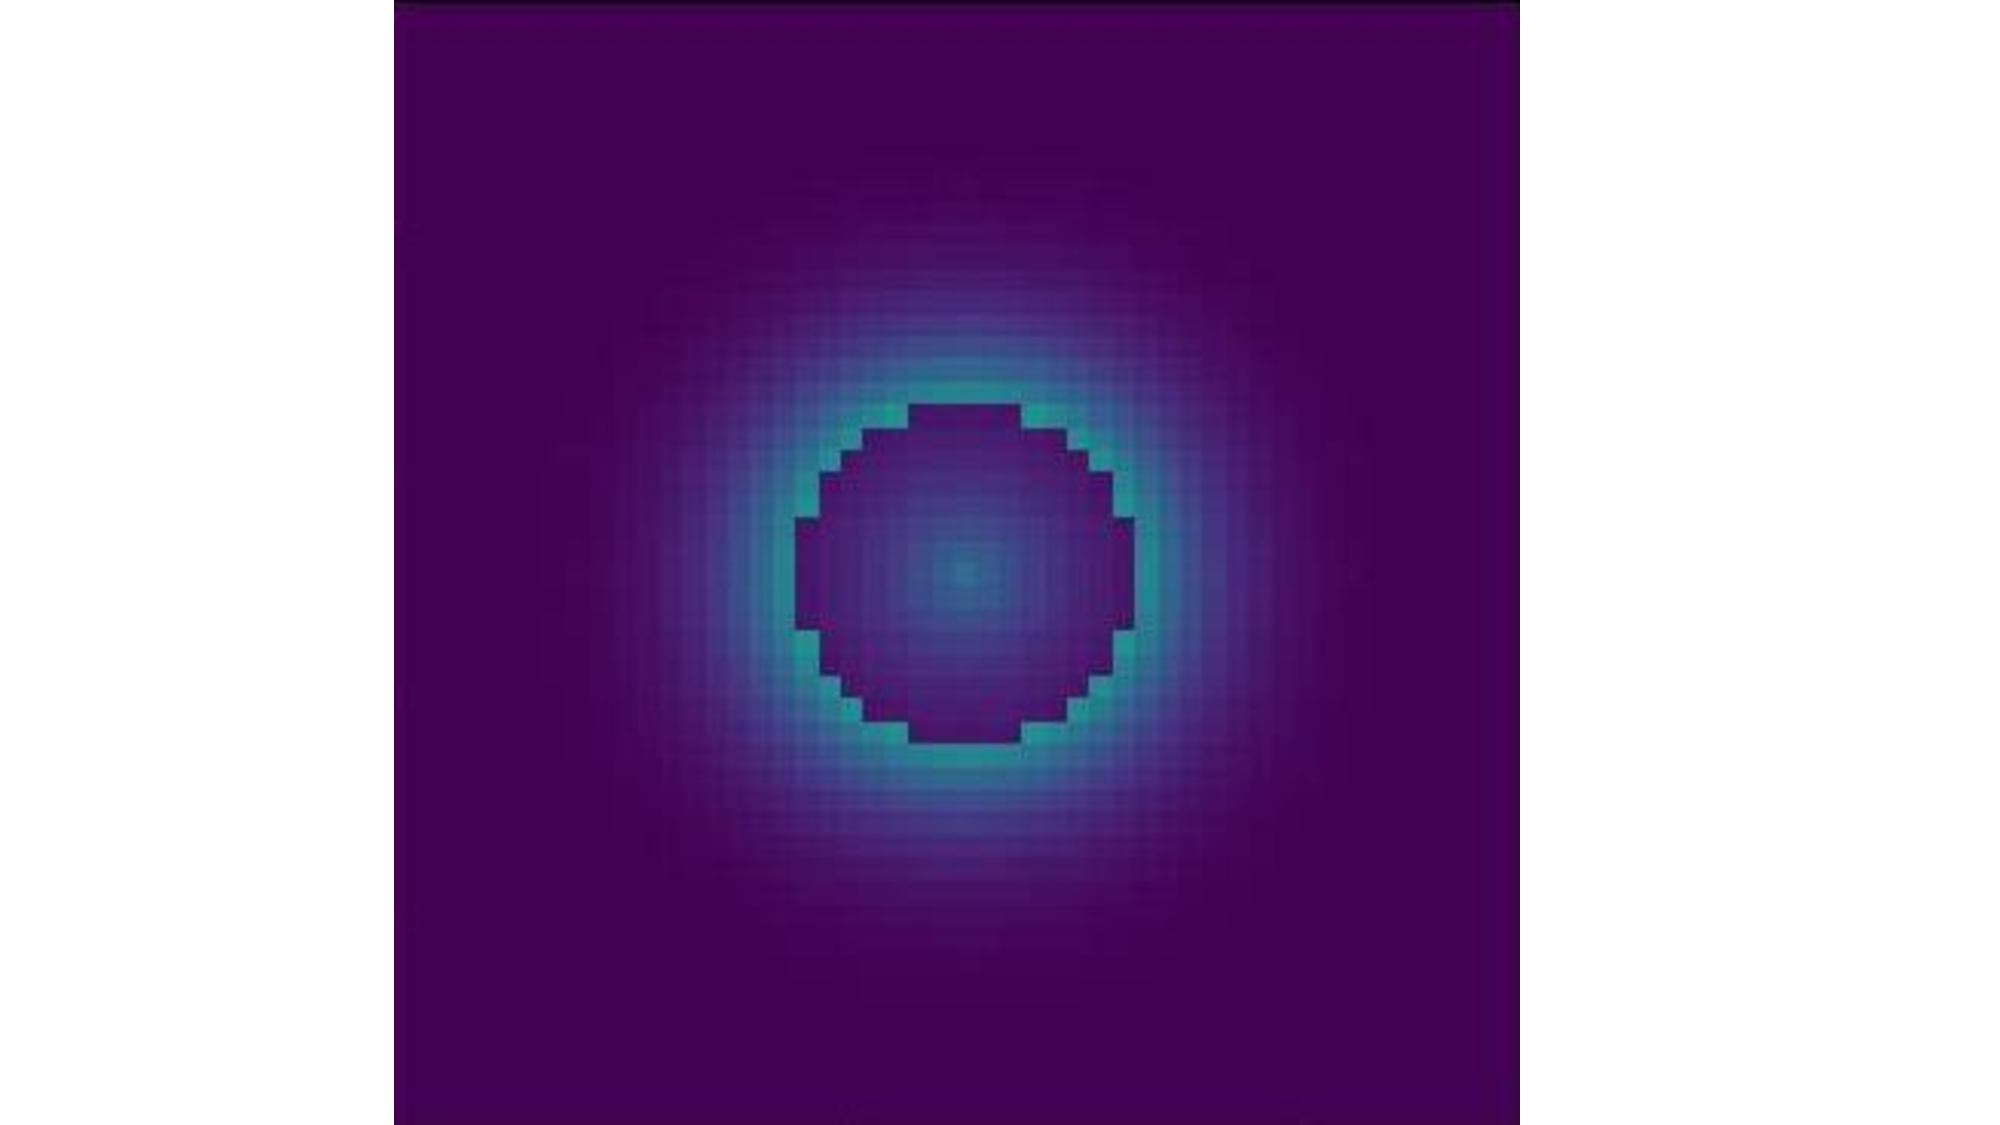
\includegraphics[width=\textwidth]{figures/raw_data/21/channel_1.pdf}
            \caption{Channel 1}
        \end{subfigure}
        \begin{subfigure}{0.23\textwidth}
            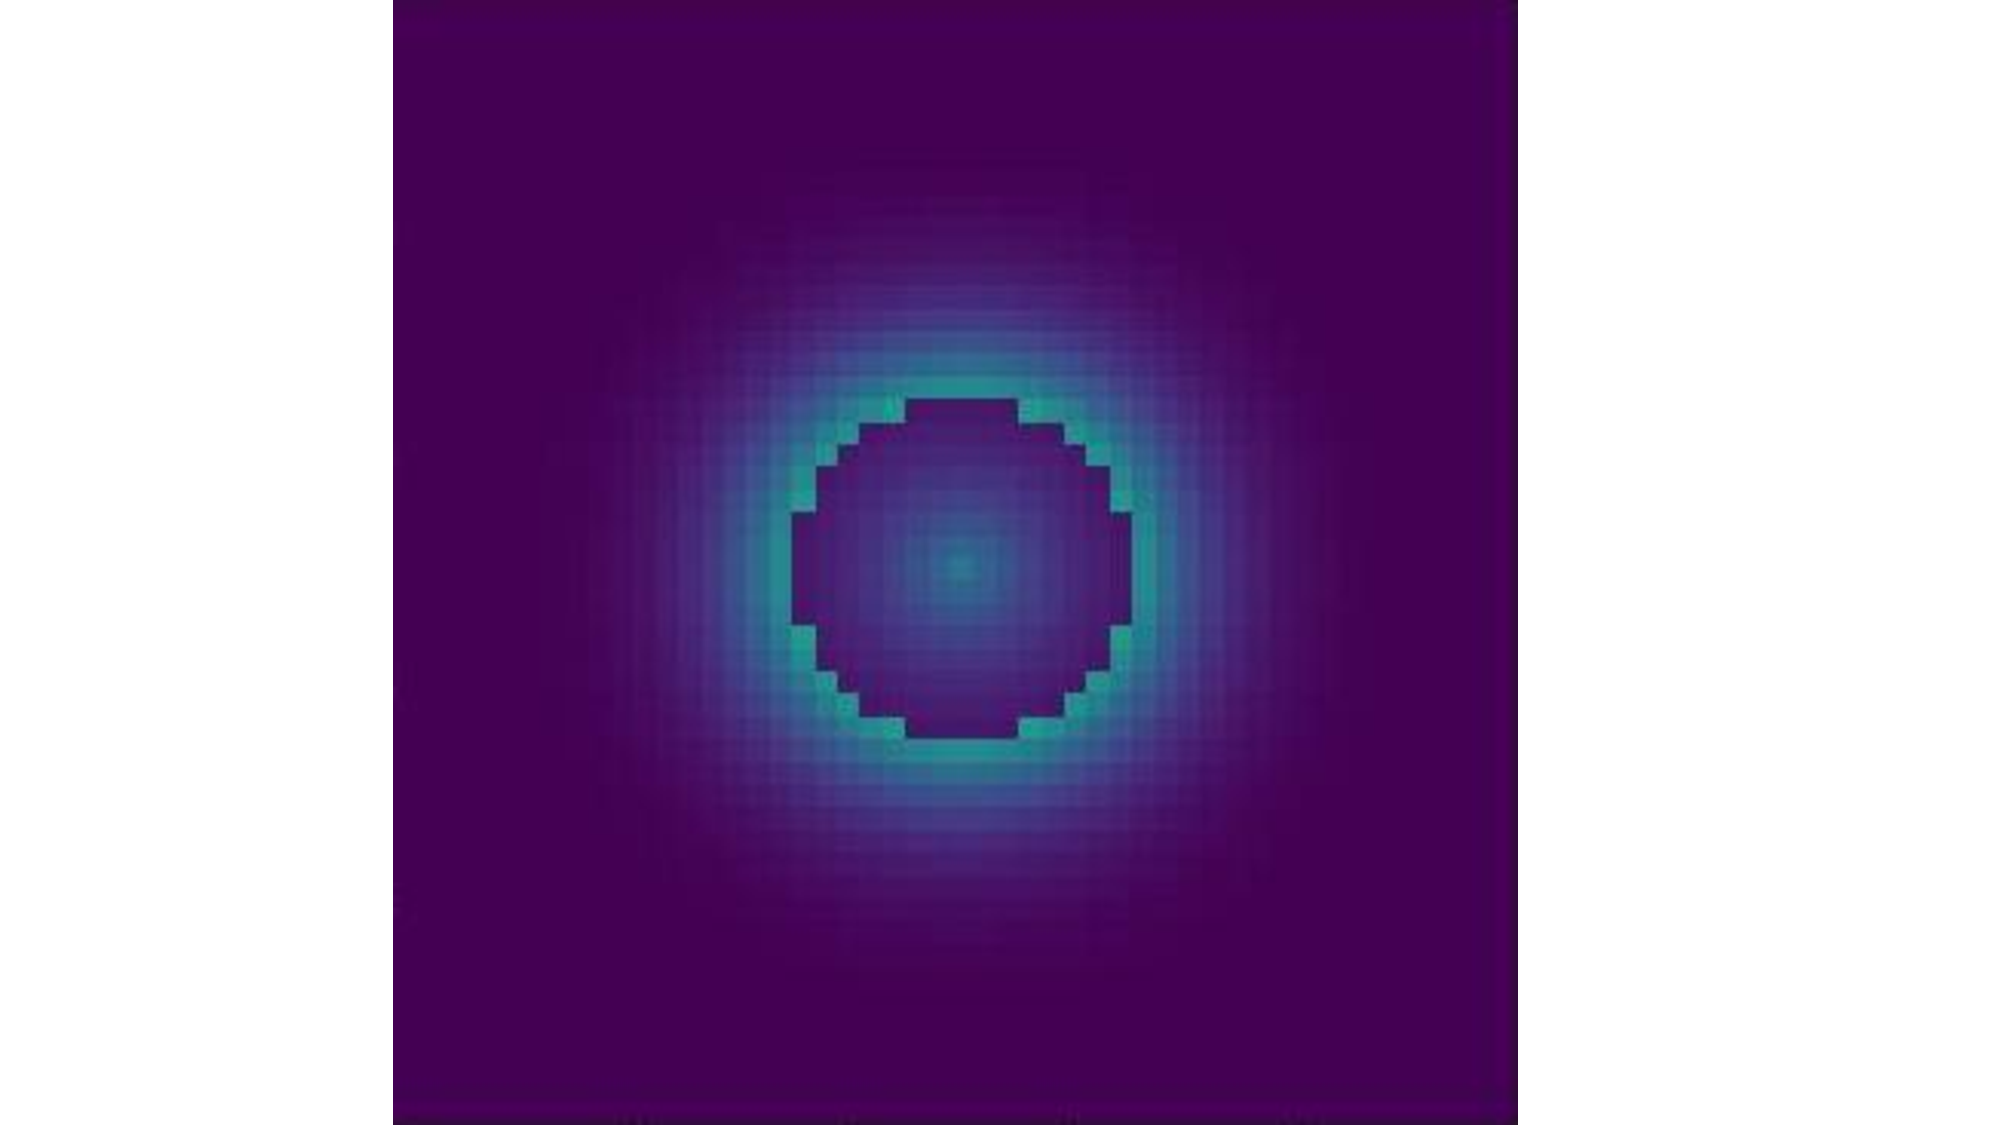
\includegraphics[width=\textwidth]{figures/raw_data/21/channel_2.pdf}
            \caption{Channel 2}
        \end{subfigure}
        \begin{subfigure}{0.23\textwidth}
            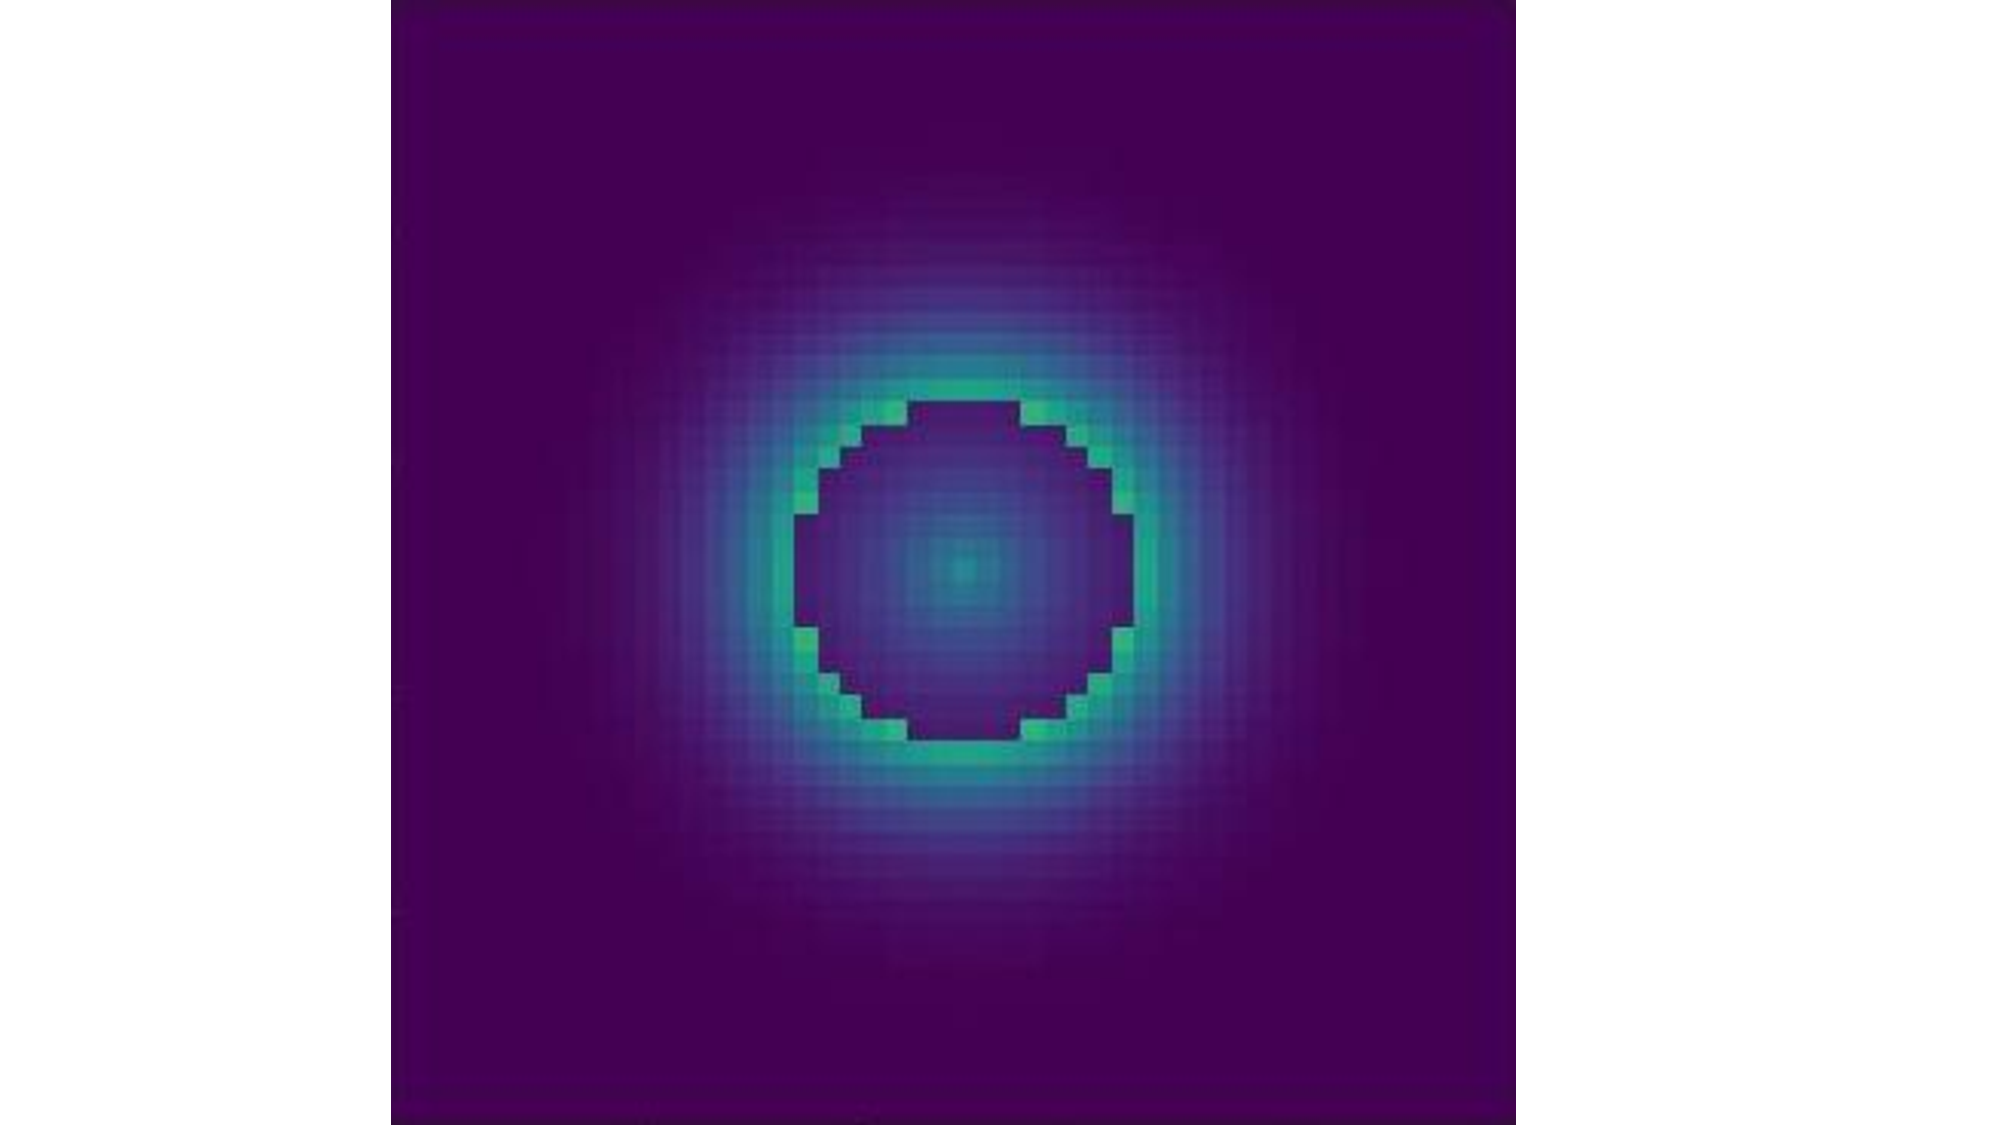
\includegraphics[width=\textwidth]{figures/raw_data/21/channel_3.pdf}
            \caption{Channel 3}
        \end{subfigure}
        \begin{subfigure}{0.23\textwidth}
            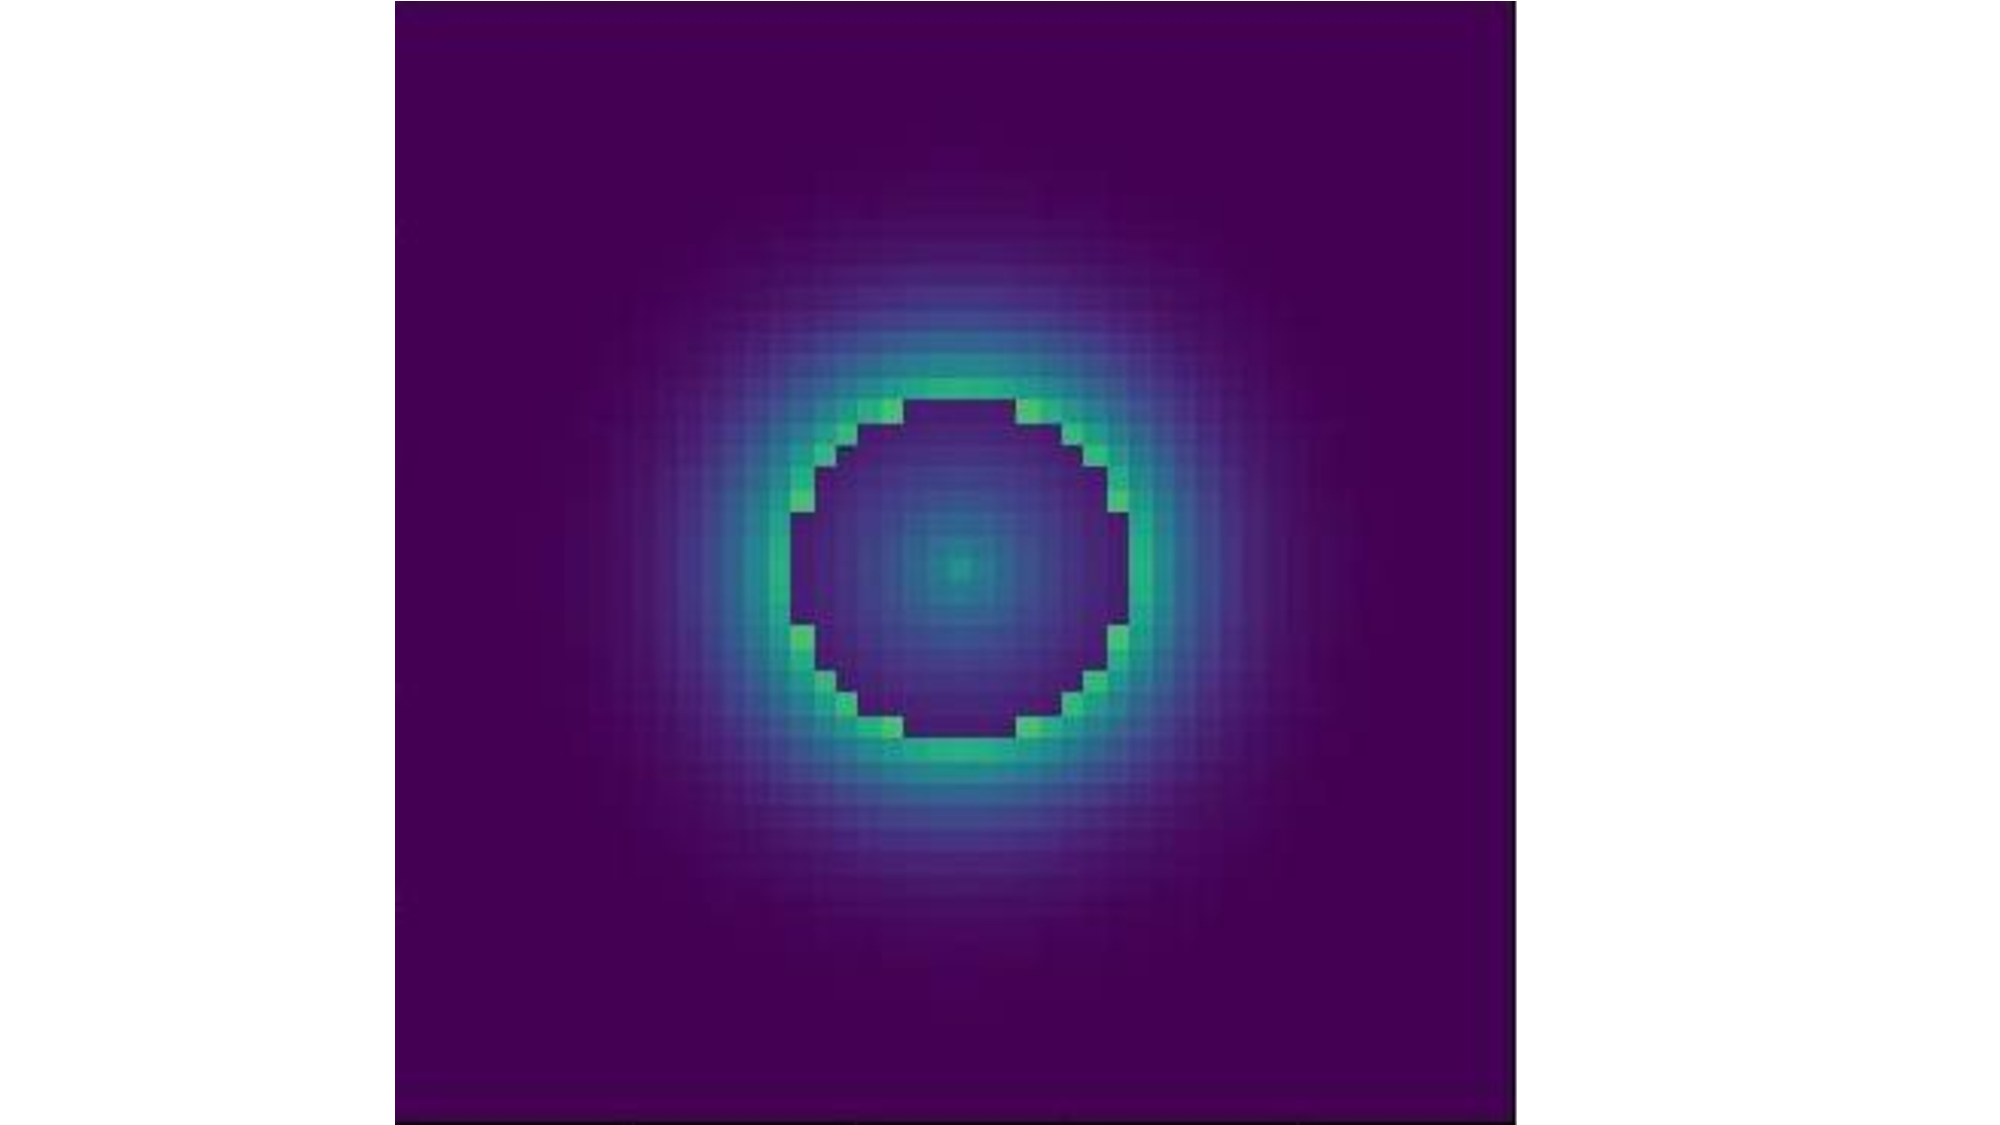
\includegraphics[width=\textwidth]{figures/raw_data/21/channel_4.pdf}
            \caption{Channel 4}
        \end{subfigure}\\
        \begin{subfigure}{0.23\textwidth}
            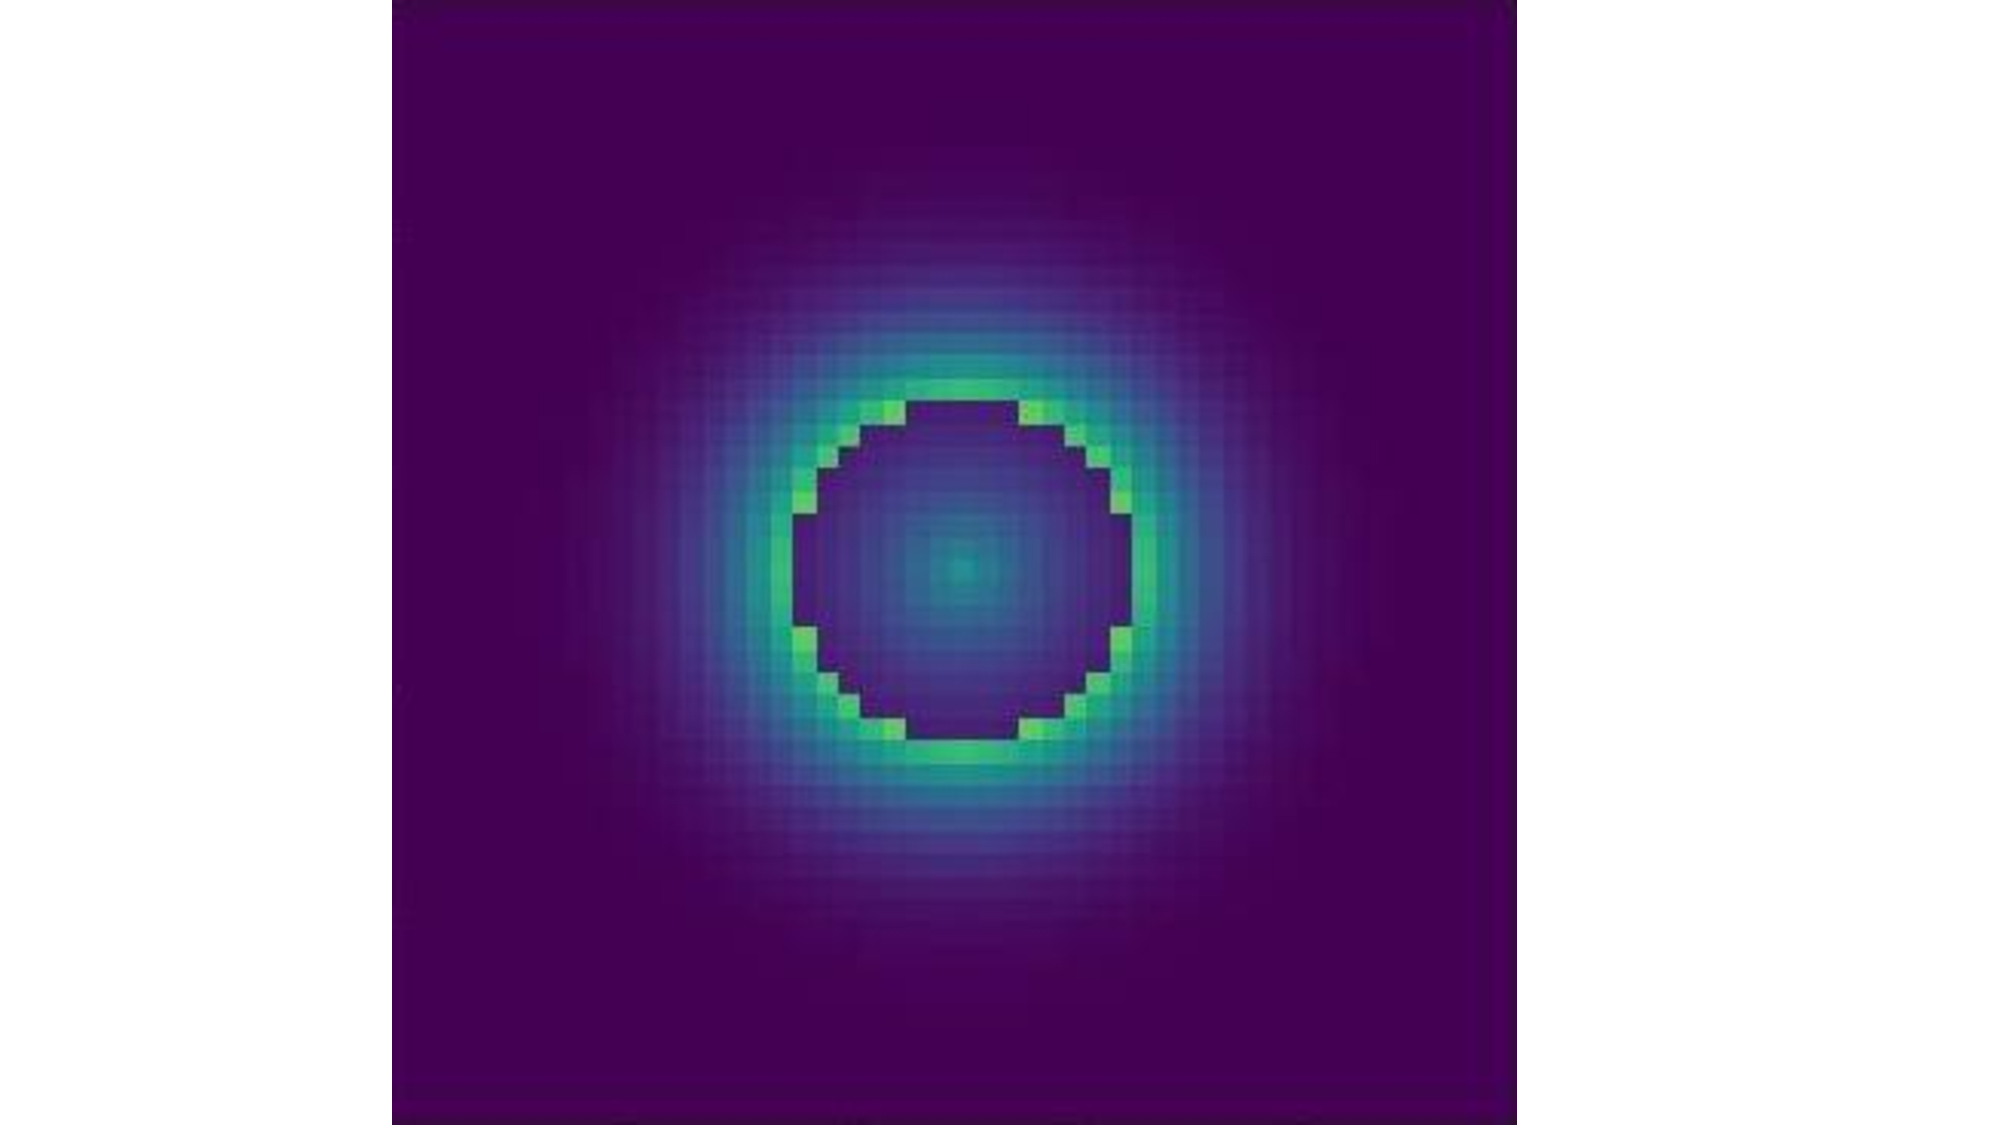
\includegraphics[width=\textwidth]{figures/raw_data/21/channel_5.pdf}
            \caption{Channel 5}
        \end{subfigure}
        \begin{subfigure}{0.23\textwidth}
            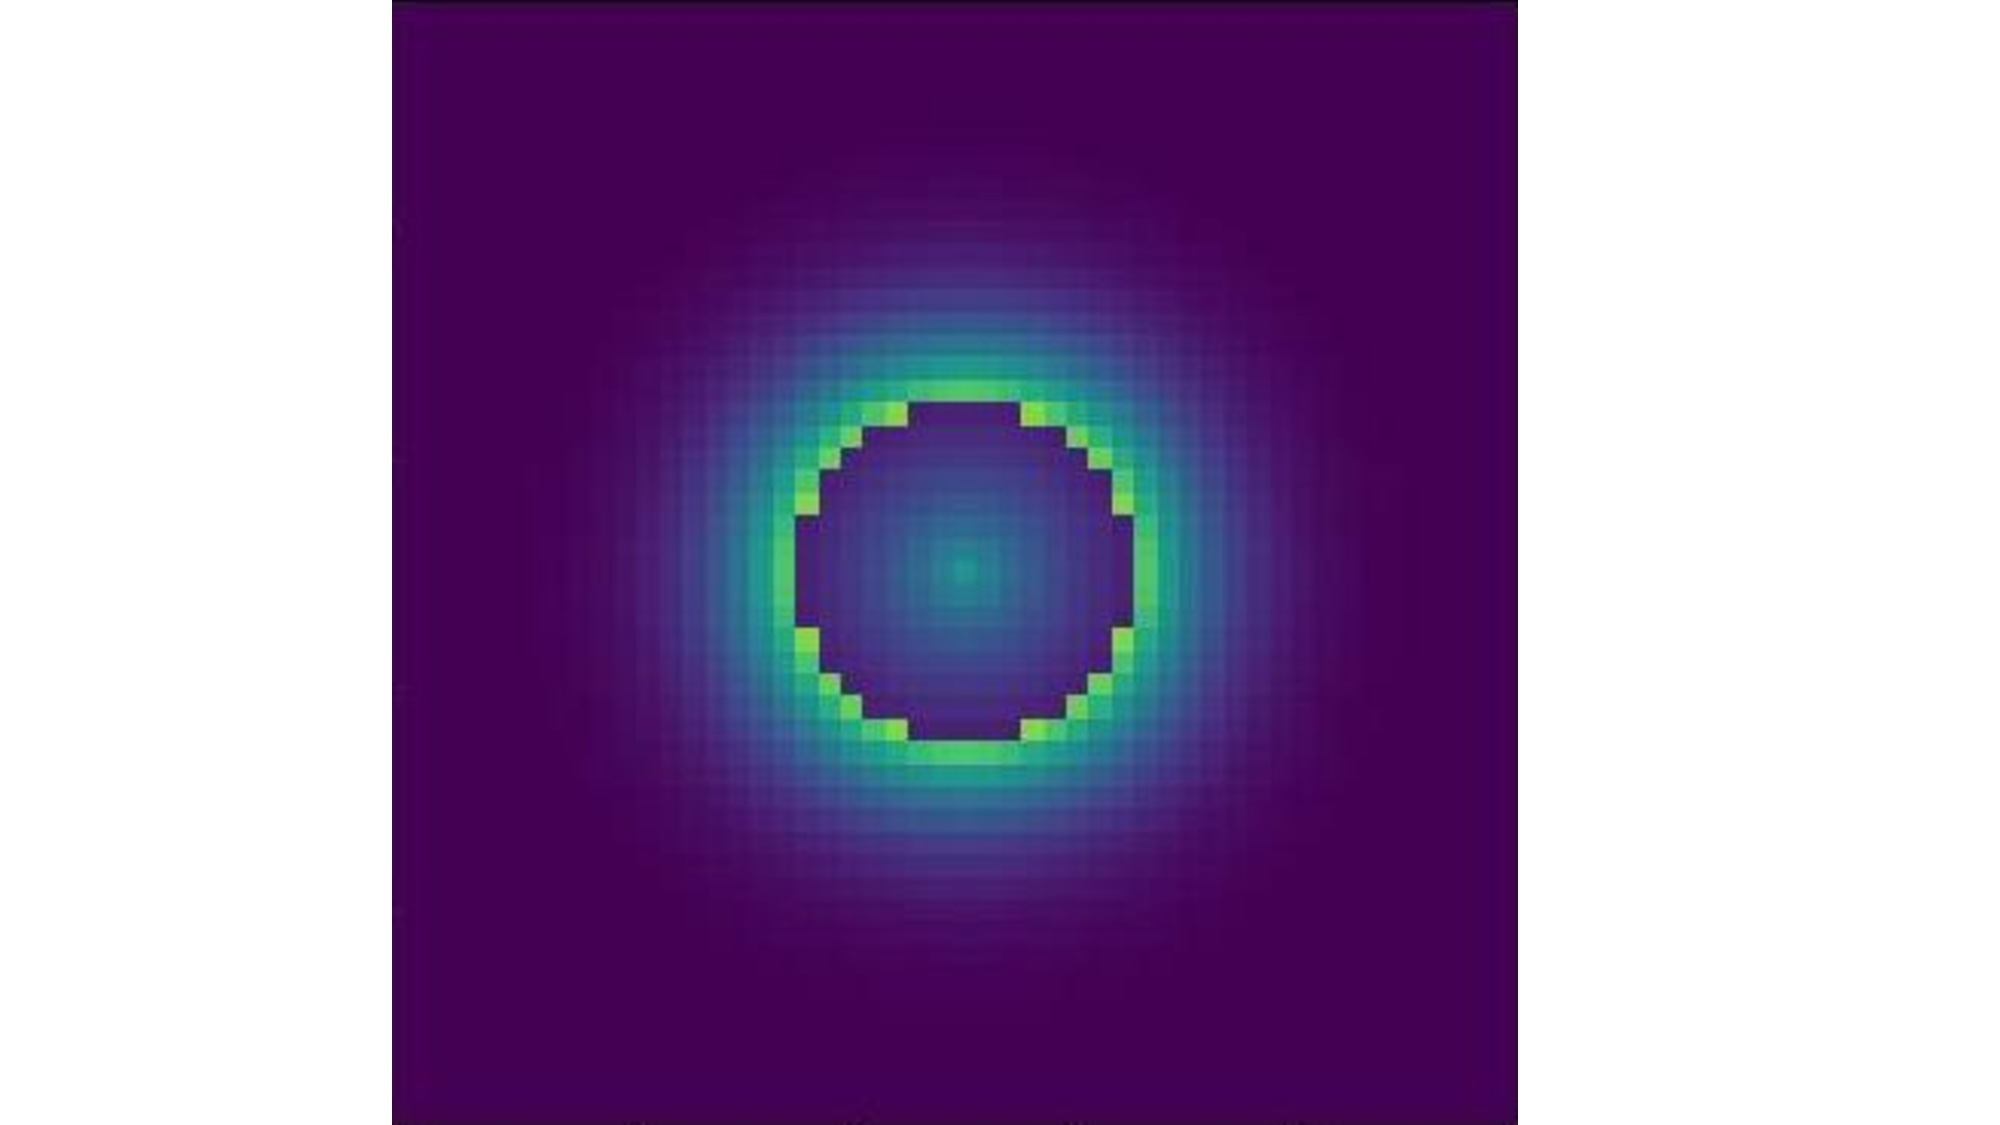
\includegraphics[width=\textwidth]{figures/raw_data/21/channel_6.pdf}
            \caption{Channel 6}
        \end{subfigure}
        \begin{subfigure}{0.23\textwidth}
            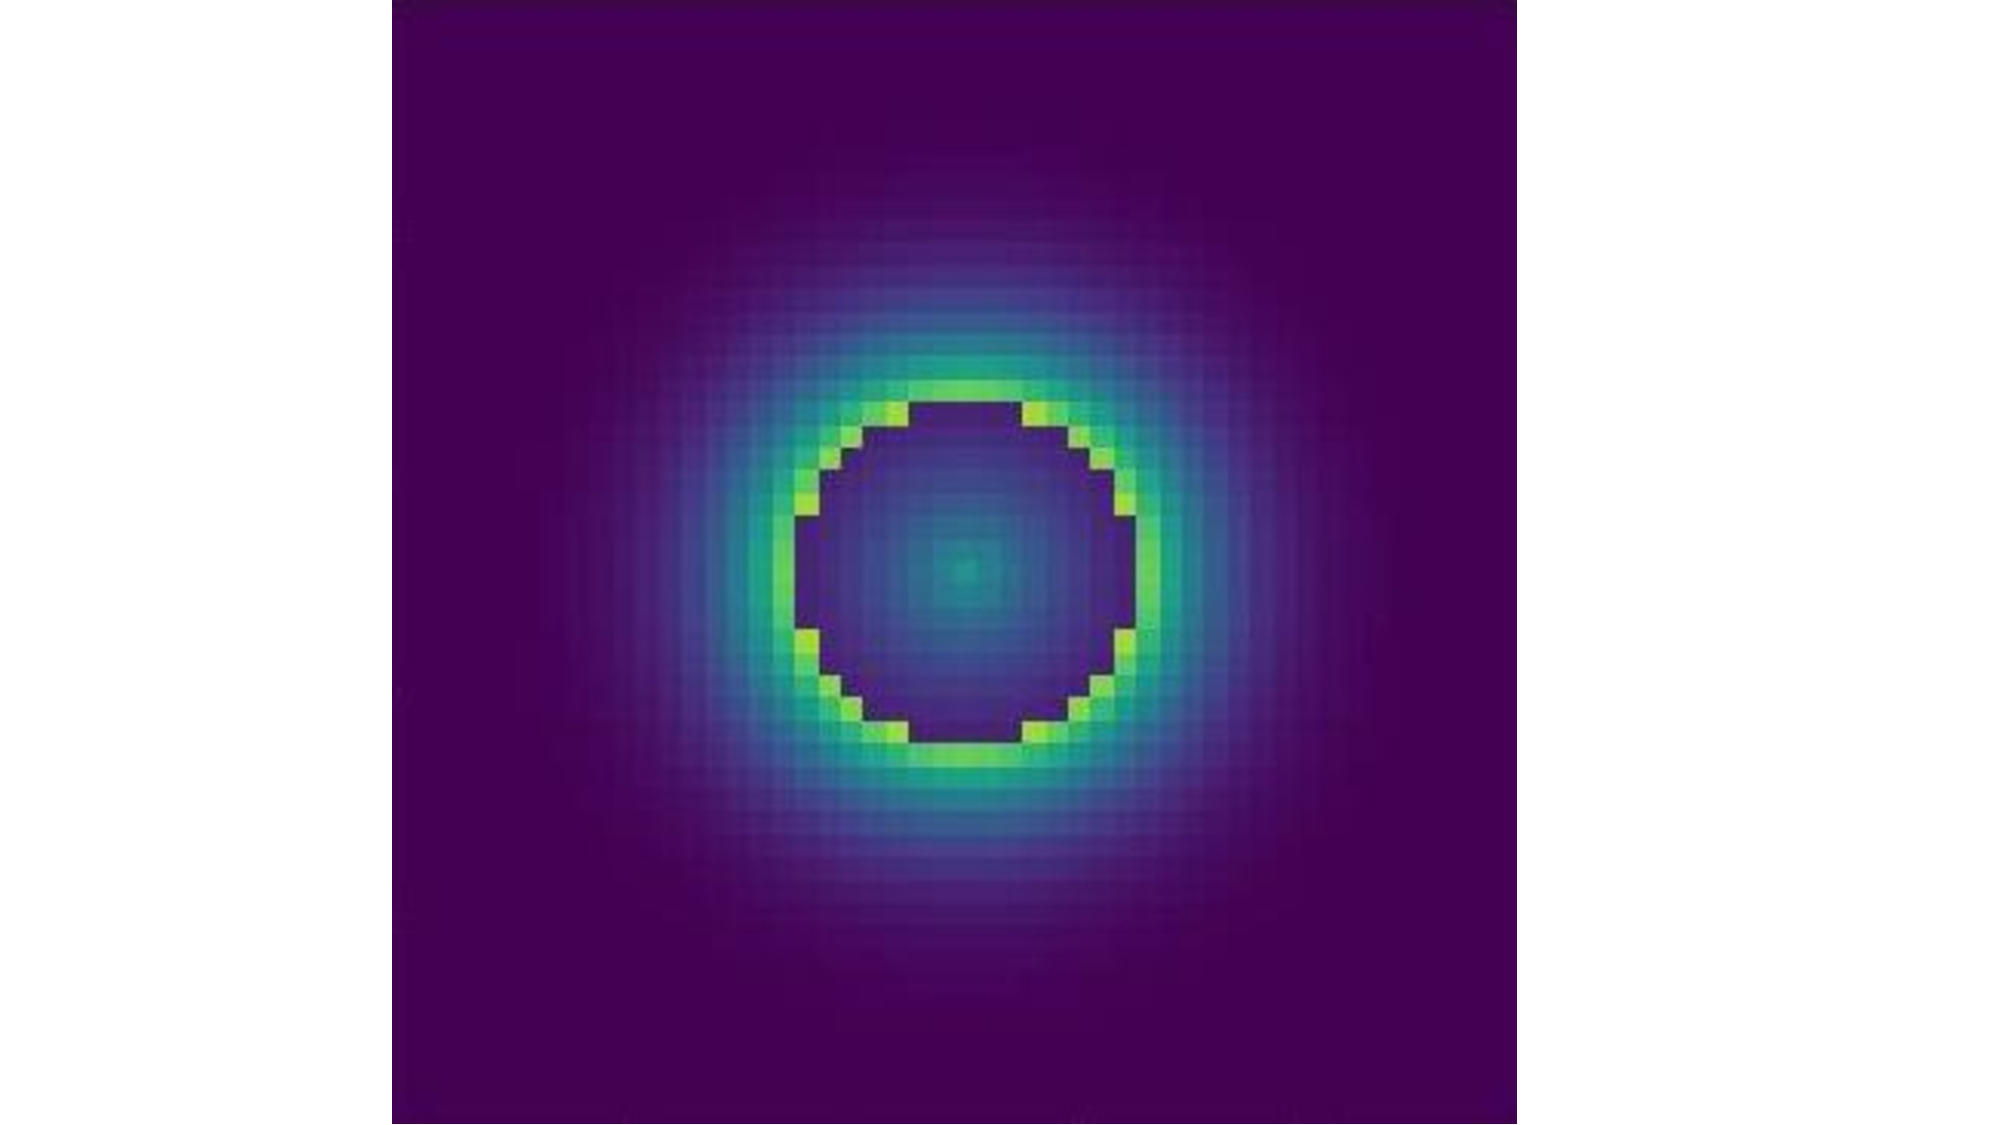
\includegraphics[width=\textwidth]{figures/raw_data/21/channel_7.pdf}
            \caption{Channel 7}
        \end{subfigure}
        \begin{subfigure}{0.23\textwidth}
            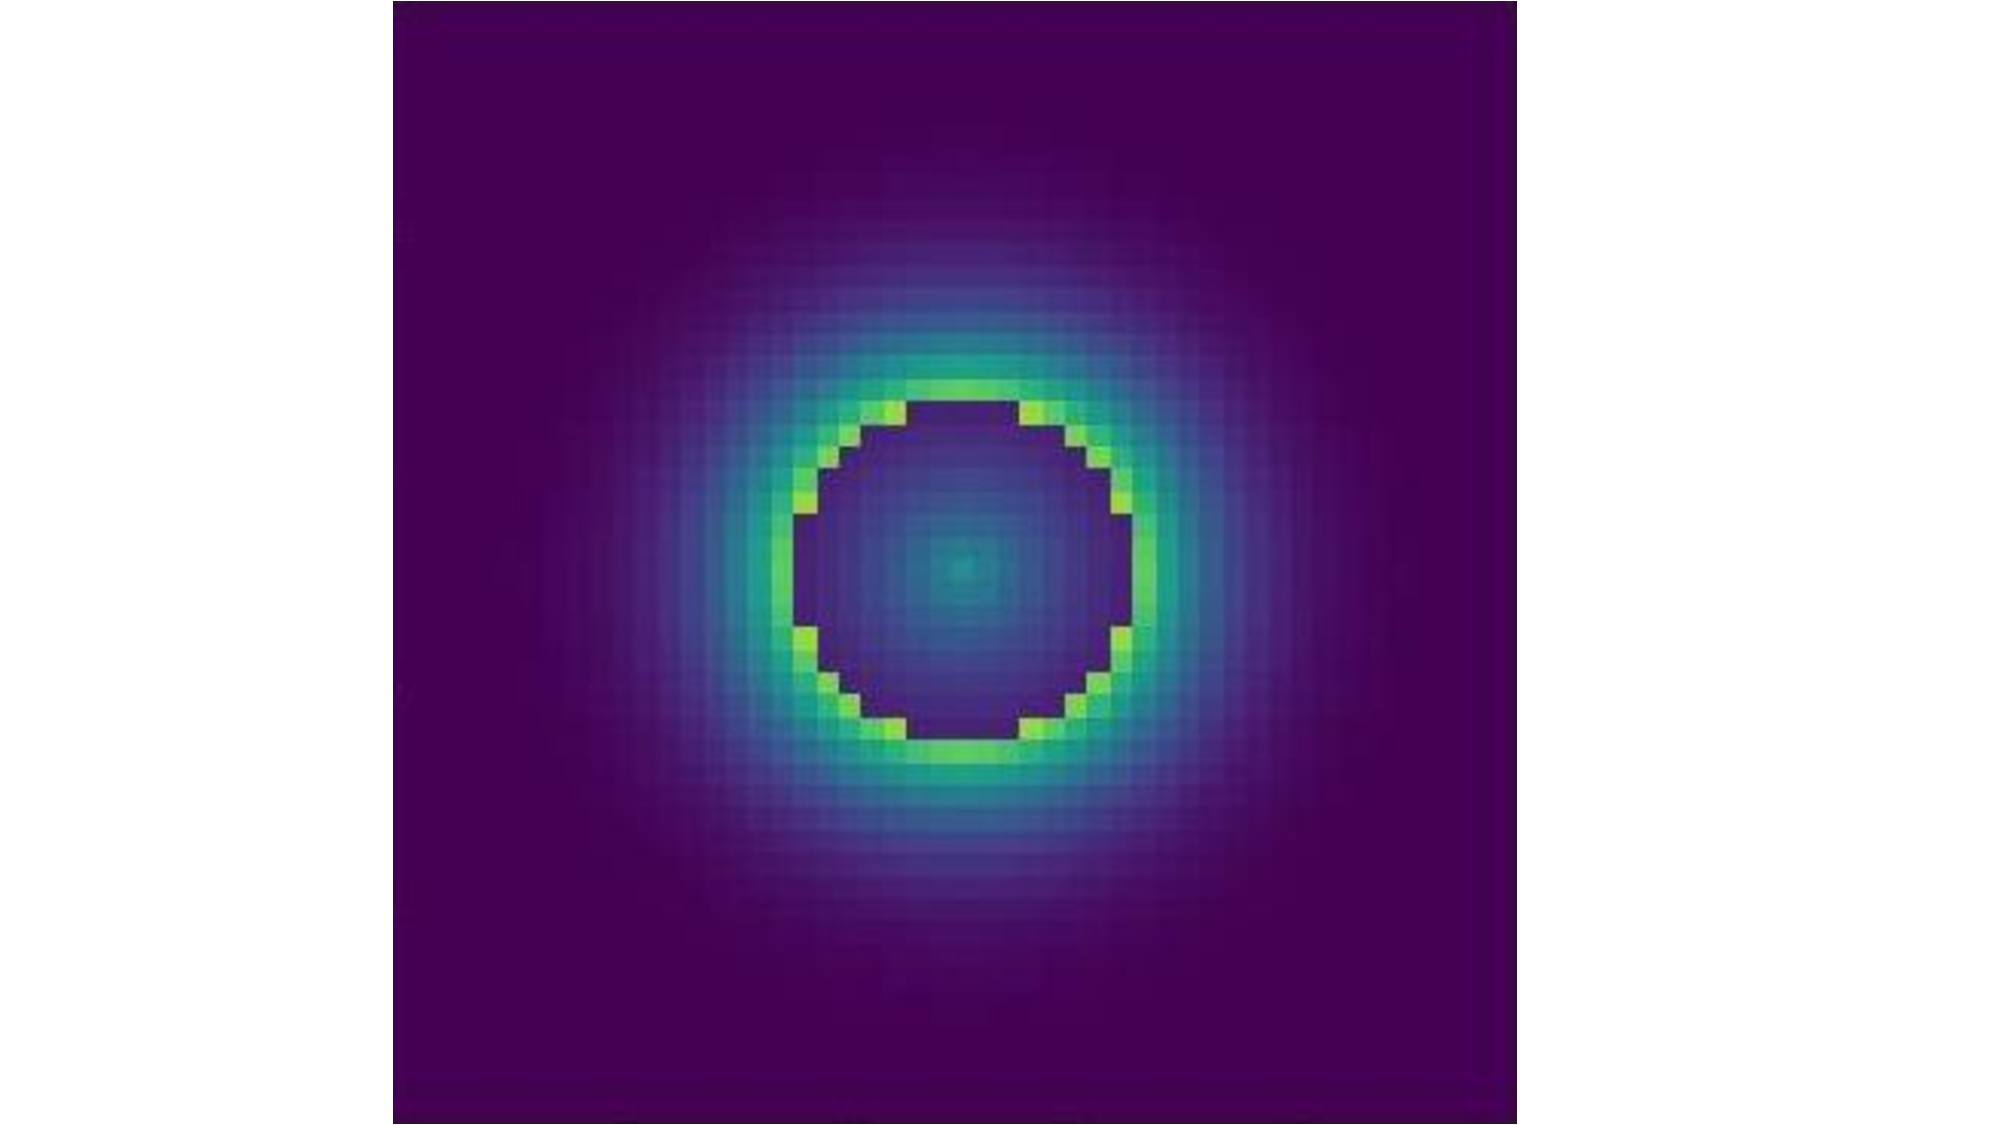
\includegraphics[width=\textwidth]{figures/raw_data/21/channel_8.pdf}
            \caption{Channel 8}
        \end{subfigure}
    \end{minipage}
    \caption{Digital value of each channel by hypothetical material based on model 1
    and a linear temperature distribution with center temperature 1900K}
    \label{fig: channel}
\end{figure}


According to Wien's displacement law introduced in previous chapter, 
as described in Eq.\ref{eq: wiens_law}, when the hypothetical material's 
temperature is 1900K, it is easy to calculate the peak 
wavelength ($\lambda_{peak}$) as 1525nm. Consequently, it can be 
inferred that the spectral intensity of blackbody radiation emitted 
by the hypothetical material will increase with increasing wavelength 
across the entire observation range ($500-1000nm$). This characteristic 
aligns with the real experimental observation, where the spectral 
radiation intensity received by a camera increases with the channel 
number.

\subsection{Estimated temperature field and emissivity field}
After obtaining reliable experimental data, it is essential to perform 
temperature estimation algorithm to validate the accuracy of the 
temperature estimation algorithm. The temperature estimation algorithm 
will yield two primary results: the estimated temperature field and the 
simplified estimated emissivity field. These computational results 
will be presented:

\begin{enumerate}
    \item Estimated temperature field: The estimated temperature field represents 
    the spatial distribution of temperature across the observation area. This is 
    a most important output of the whole temperature estimation algorithm.

    \item Simplified estimated emissivity field: The simplified estimated 
    emissivity field denotes the variation of emissivity across the 
    observation area. It could be used to indentify the phase change area 
    and thus find the improvement potential.
\end{enumerate}


For visualization, the presentation of the computational results will be categorized based on the 
emissivity model used in the temperature estimation algorithm. As the 
experimental data for these temperature estimation algorithm use the 
same temperature distribution, relative error of temperature is employed here to 
represent the accuracy of the computations. To save space, the results 
of calculations for blackbody materials and materials based on Model 1 are selected for presentation.


In real experimental data, due to the limitations of the sensors, it is not 
possible to simultaneously observe the radiation intensity of the non-laser-heated 
region and the radiation intensity of the laser-heated region. In the 
virtual experimental platform, the temperature of the background region is 
assumed to be uniform, which is comparable to the real situations. 
Consequently, in order to avoid introducing statistical errors, the calculation 
results of the temperature estimation algorithm in background region can be 
considered as negligible.

\subsubsection{Linear model}

\begin{figure}[htbp]
    \centering
    \begin{minipage}{\textwidth}
        \centering
        \begin{subfigure}{0.325\textwidth}
            \centering
            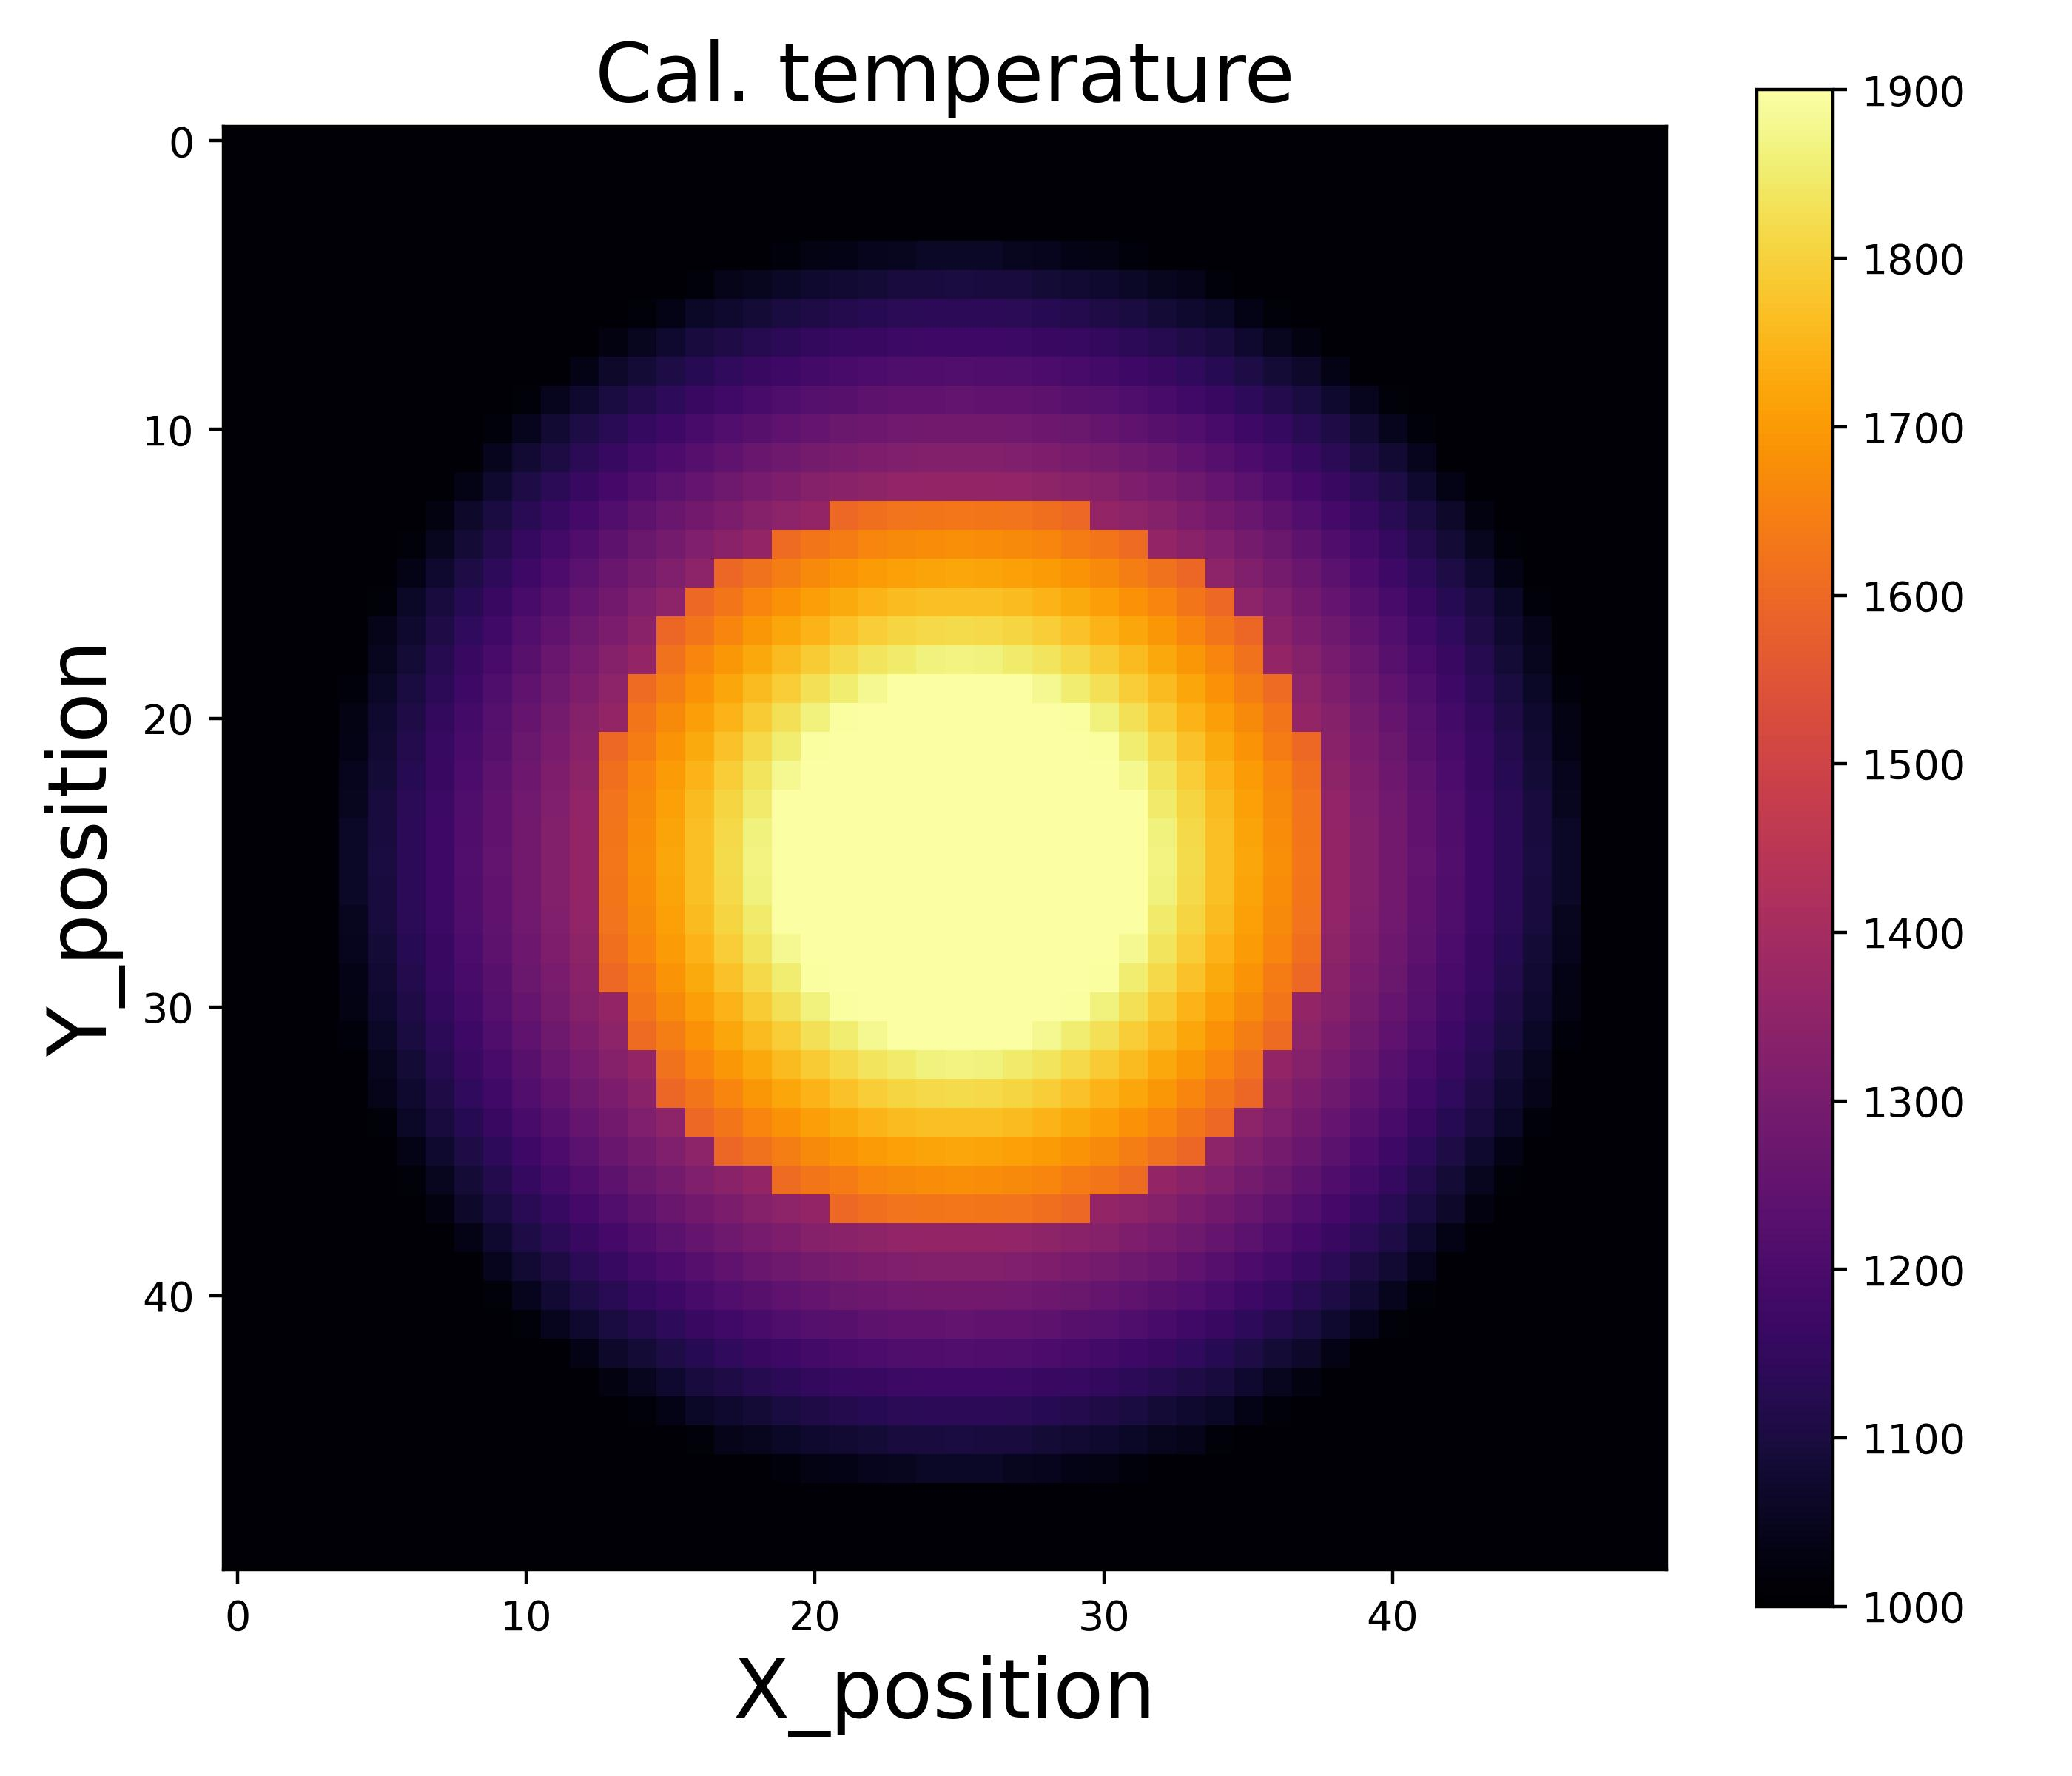
\includegraphics[width=\textwidth]{figures/raw_data/21/linear/T_cal.jpg}
        \end{subfigure}
        \begin{subfigure}{0.325\textwidth}
            \centering
            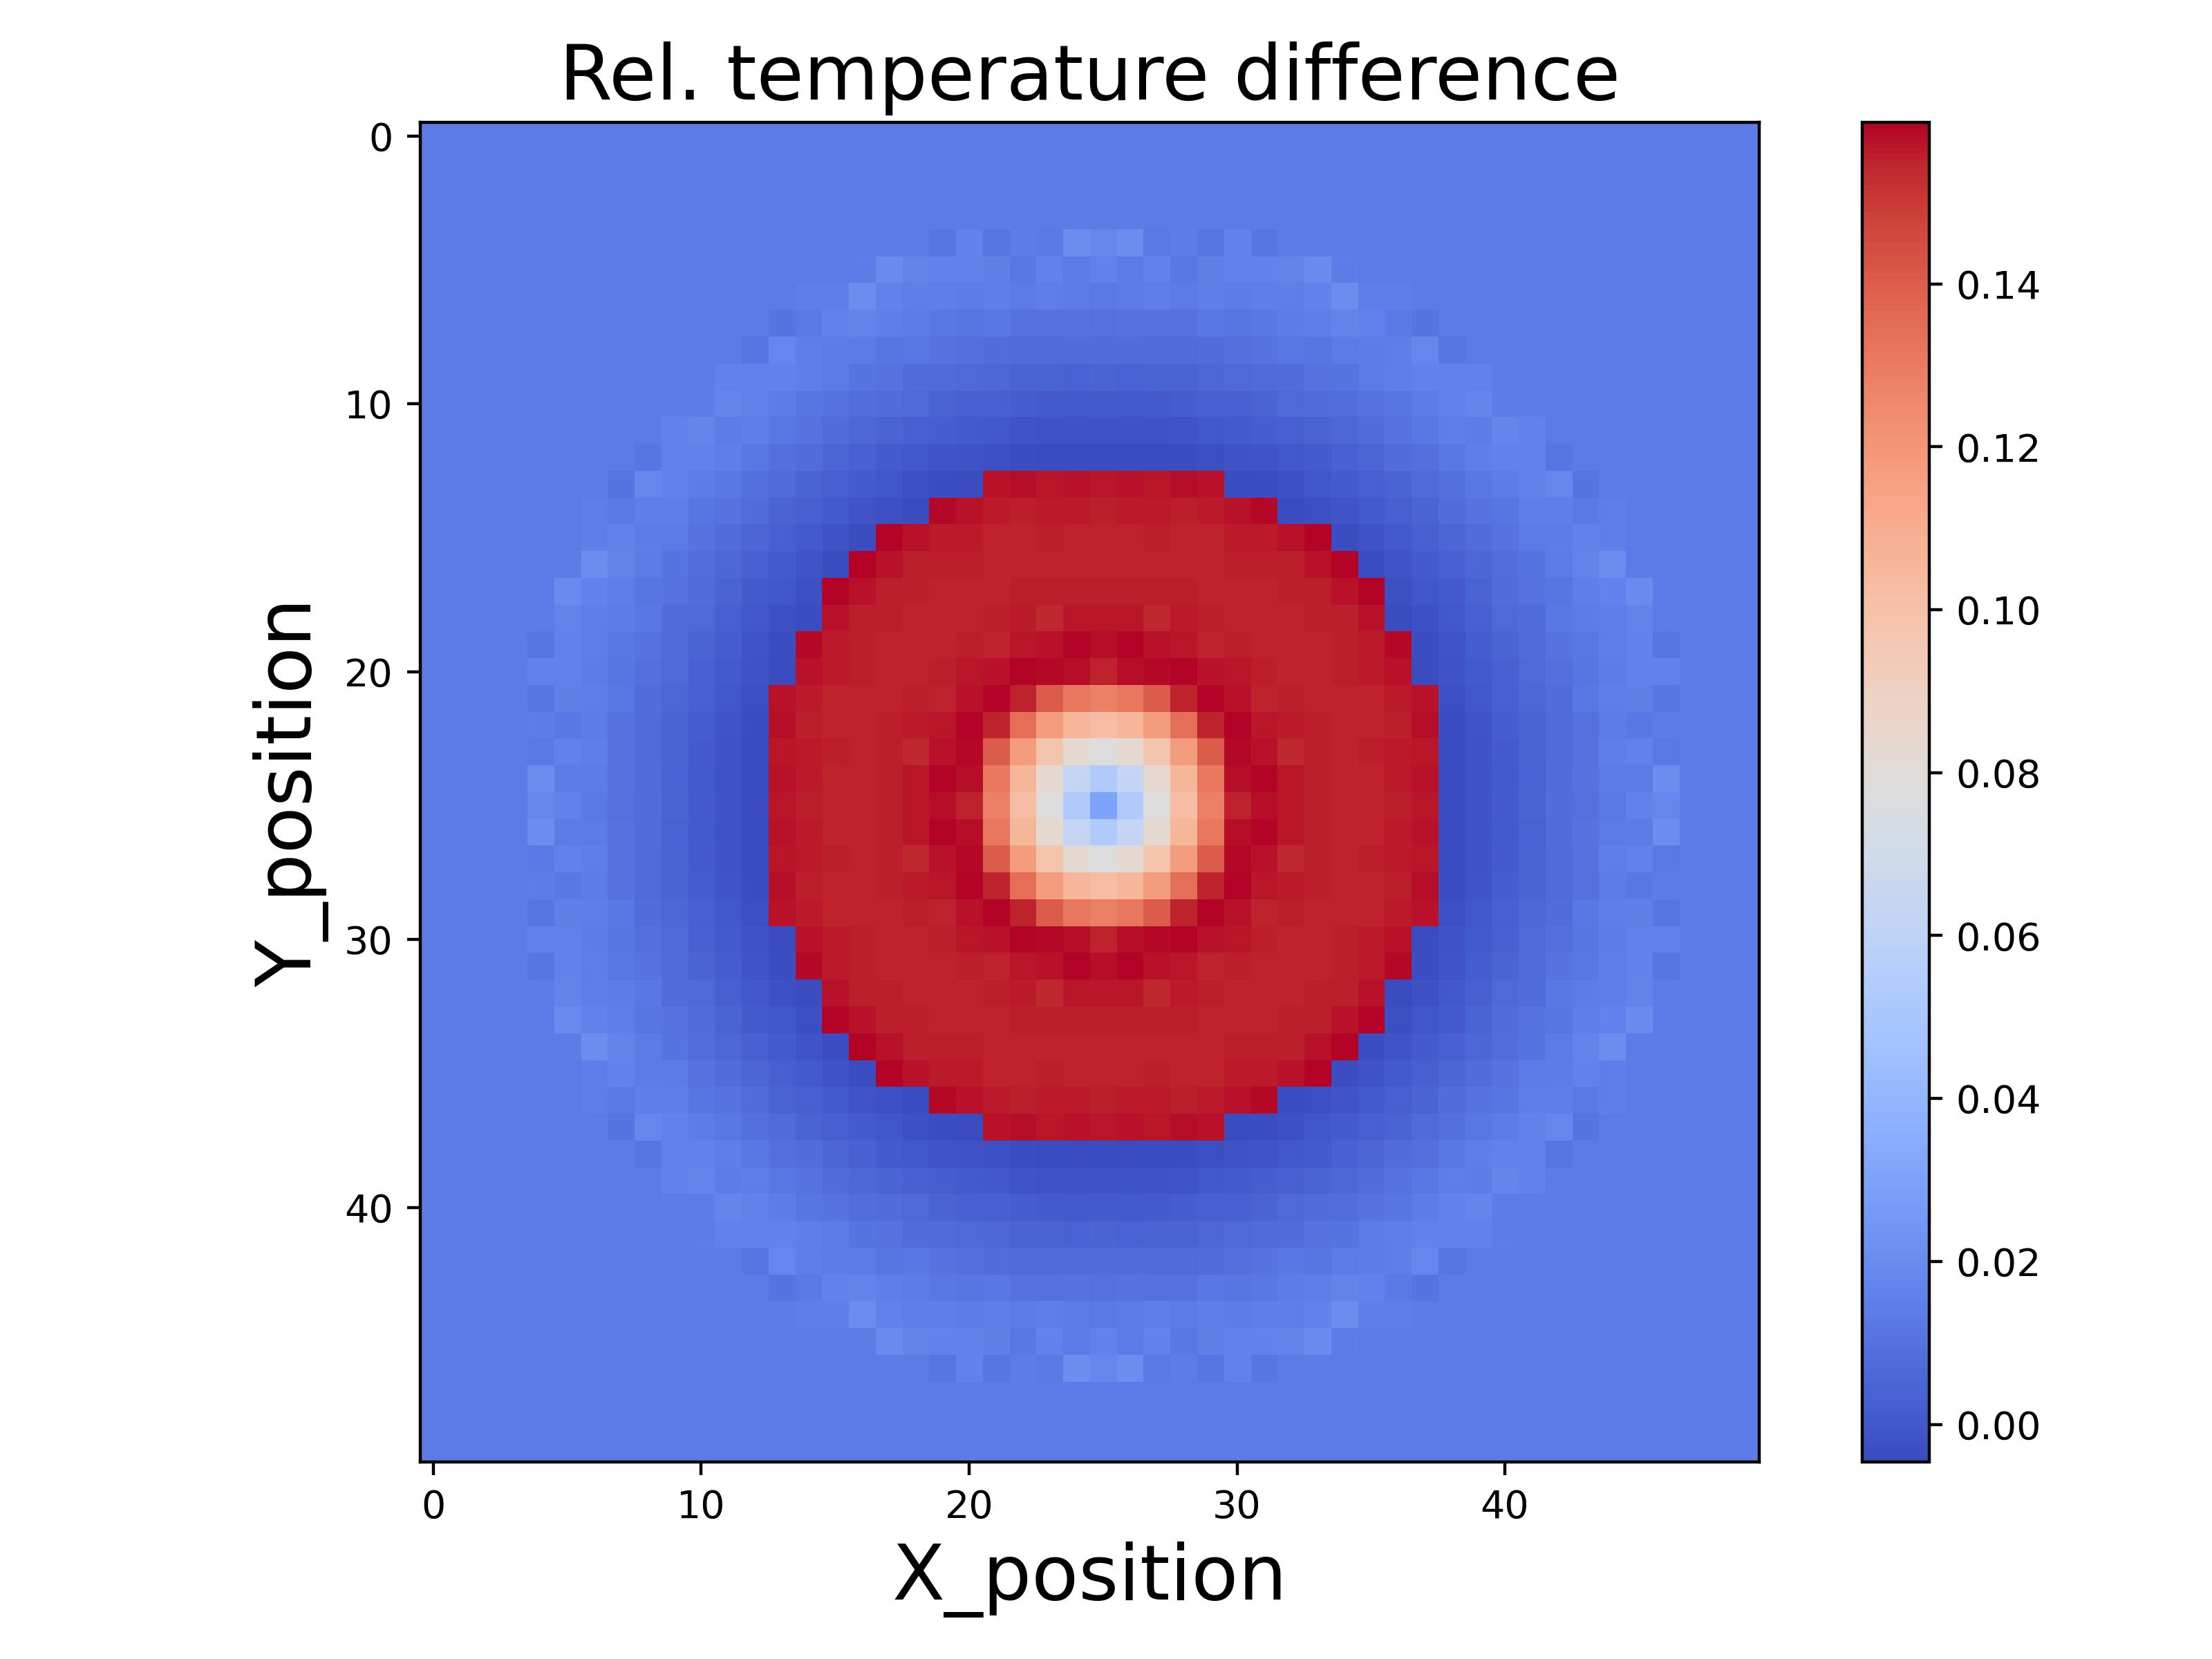
\includegraphics[width=\textwidth]{figures/raw_data/21/linear/T_bias.jpg}
        \end{subfigure}
        \begin{subfigure}{0.325\textwidth}
            \centering
            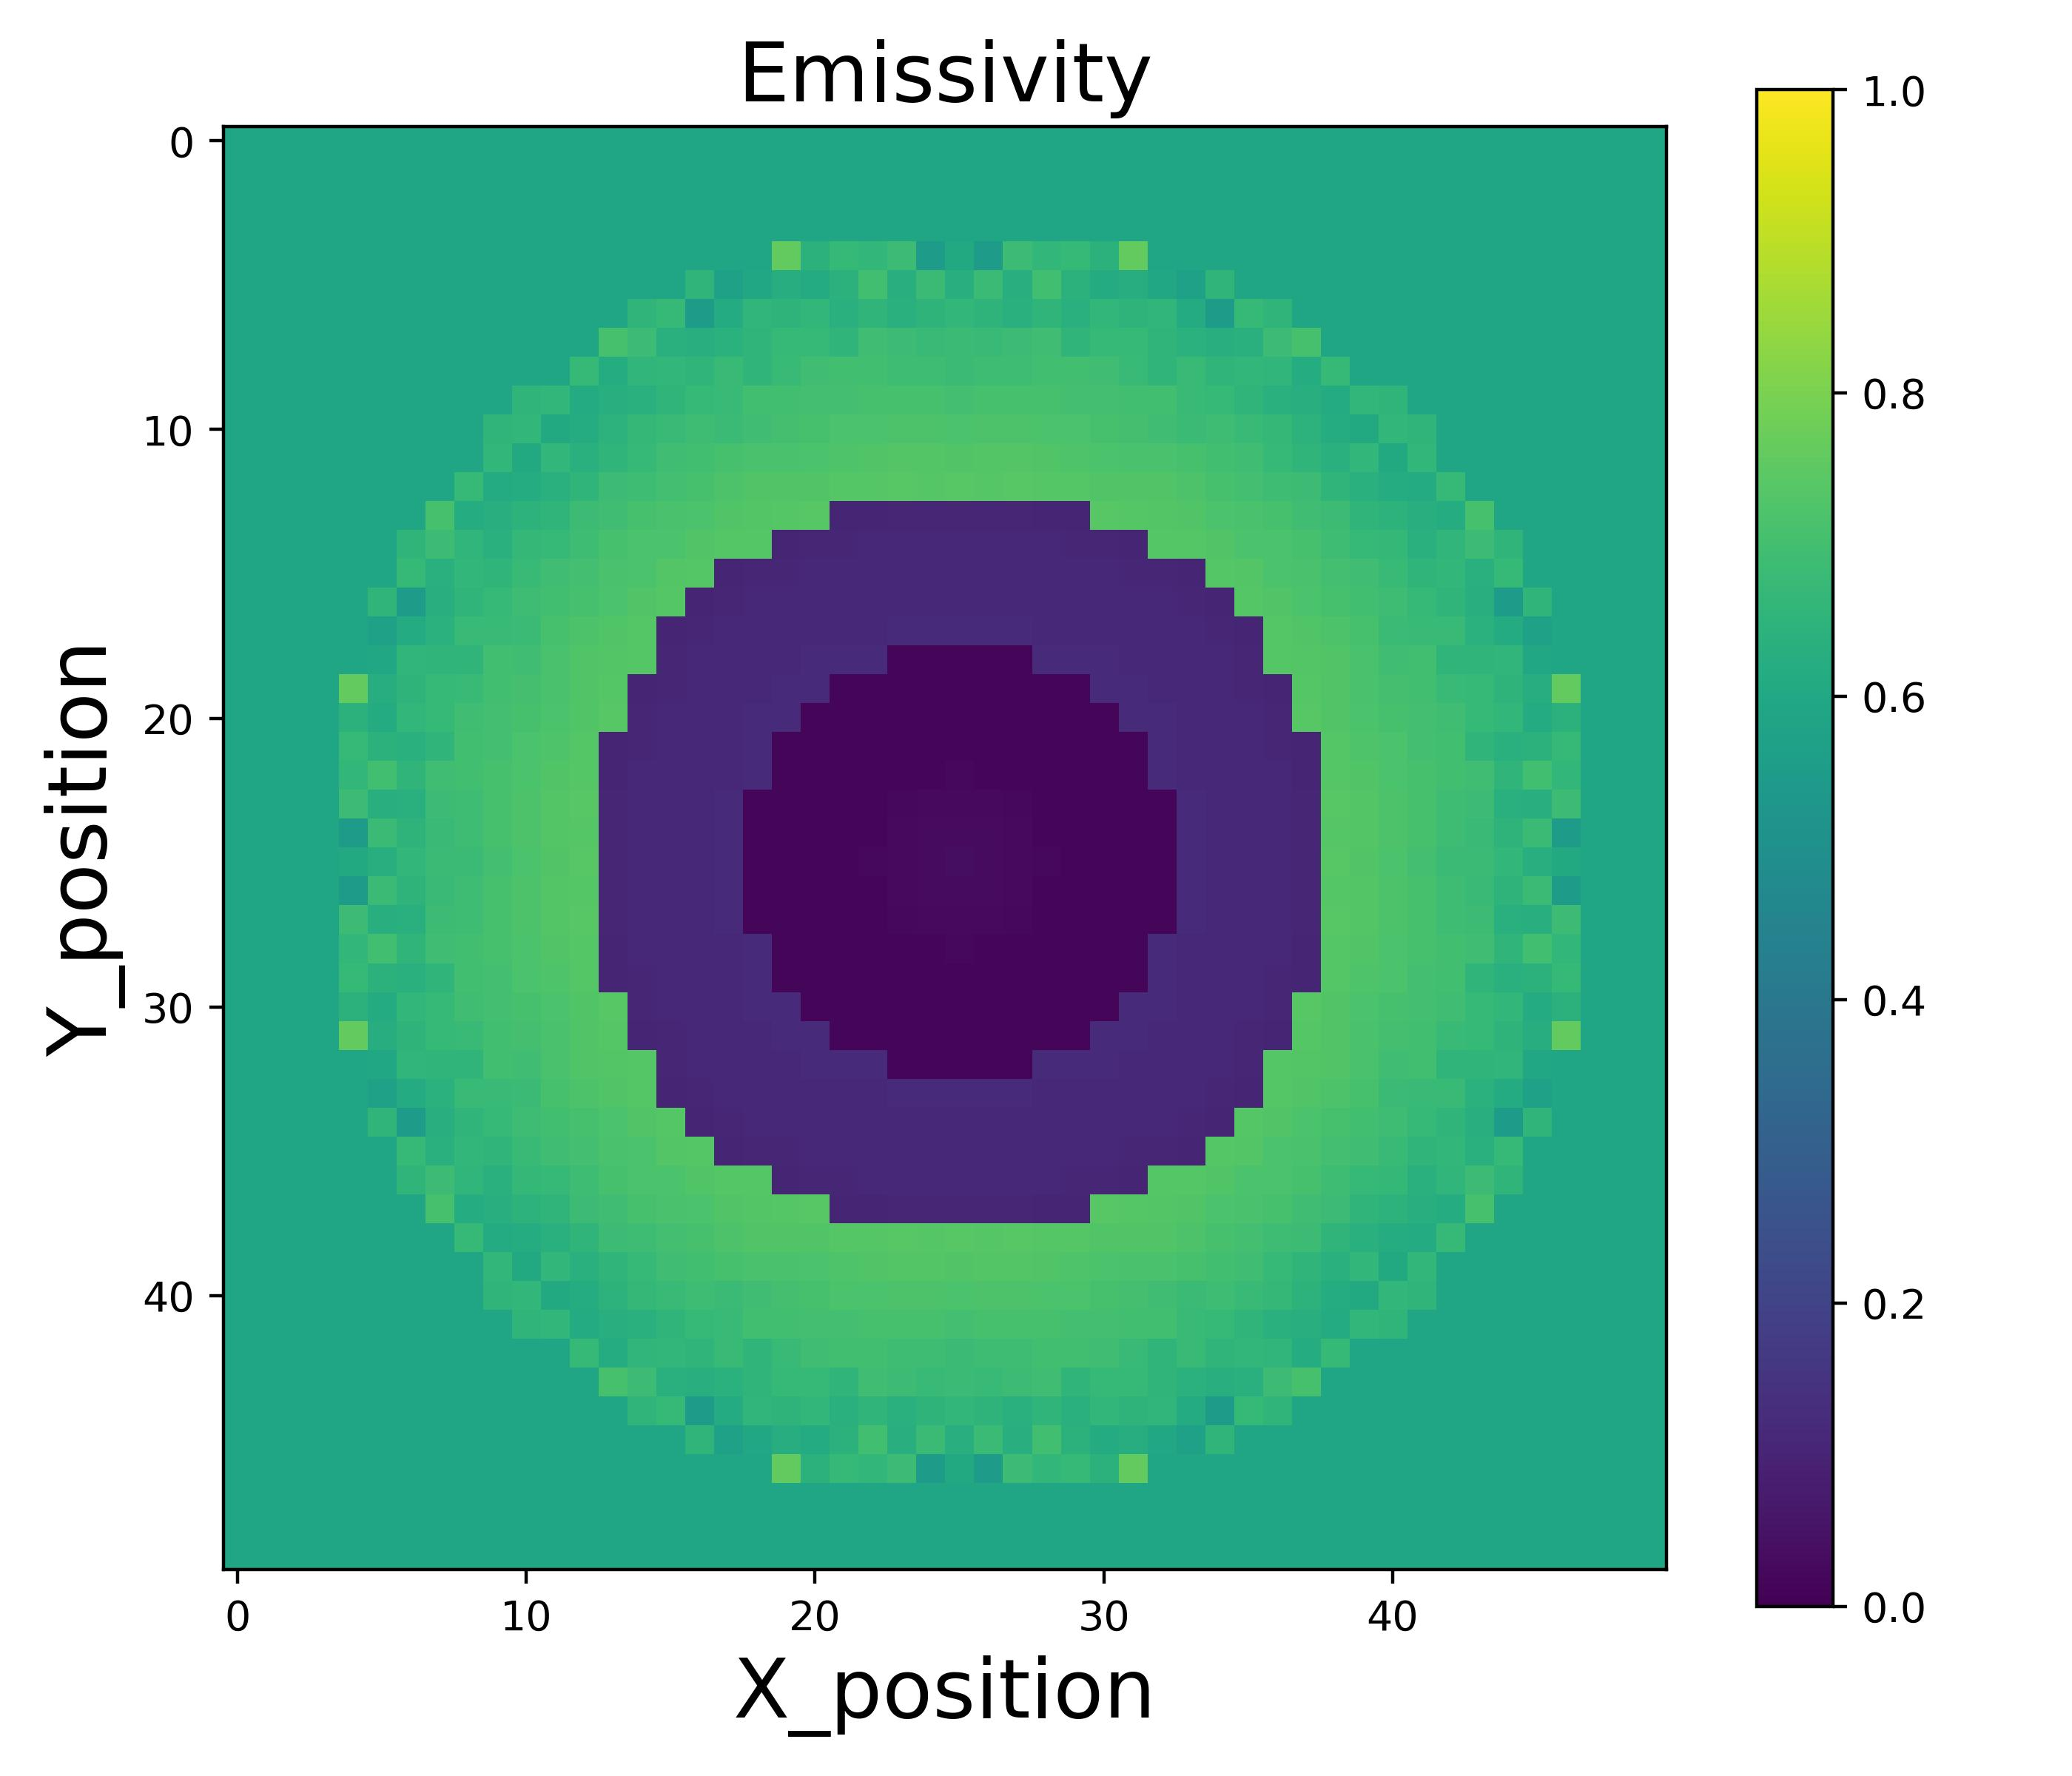
\includegraphics[width=\textwidth]{figures/raw_data/21/linear/emi_cal.jpg}
        \end{subfigure}
        \subcaption{Material based on model 1}
    \end{minipage}\\
    \begin{minipage}{\textwidth}
        \centering
        \begin{subfigure}{0.325\textwidth}
            \centering
            \includegraphics[width=\textwidth]{figures/raw_data/5/linear/T_cal.jpg}
        \end{subfigure}
        \begin{subfigure}{0.325\textwidth}
            \centering
            \includegraphics[width=\textwidth]{figures/raw_data/5/linear/T_bias.jpg}
        \end{subfigure}
        \begin{subfigure}{0.325\textwidth}
            \centering
            \includegraphics[width=\textwidth]{figures/raw_data/5/linear/emi_cal.jpg}
        \end{subfigure}
        \subcaption{Material based on real iron data}
    \end{minipage}
    \caption{Calculation results of linear model}
    \label{fig: result_linear_model}
\end{figure}


Fig.\ref{fig: result_linear_model} demonstrate the calculation result on material based on 
model 1 and real data from iron. It can be found that the calculation result is more
stable in real data due to the material character. 


It can be observed that relative bias are present 
in the estimations based on two different materials. Moreover, this relative bias 
experiences a sudden change with increasing temperature, represented by a red 
circle in the figure. The reason behind this phenomenon can be considered as follows, 
at the boundary of the circle, the material undergoes a phase change from solid to liquid, 
leading to a rapid change in emissivity. The linear model is only able to  
simulate linear emissivity models, which fails to adequately fit the variations 
occurring at this point, resulting in significant deviations in the 
temperature estimations.


It can be found in table \ref{tab: statistic_results} that in the computation of linear models, 
calculation results based on real data exists relatively low average relative error and the lowest 
standard deviation. This indicates that the linear model maintains a higher 
level of consistency when performing calculations on real materials. It also 
achieves a maximum relative error of no more than 9.6\%. However, when 
performing calculations on other hypothetical materials, the linear model may 
produce relatively large errors, particularly for model 8, which has a high standard 
deviation, meaning the low consistency in the calculations. As mentioned 
in previous sections, this decrease in computational consistency could be attributed to the 
fact that the emissivity of materials based on model 8 undergoes a sudden change 
as the wavelength increases, which is a potential reason for the decline in 
calculation consistency.


\subsubsection{Linear square model}

\begin{figure}[htbp]
    \centering
    \begin{minipage}{\textwidth}
        \centering
        \begin{subfigure}{0.325\textwidth}
            \centering
            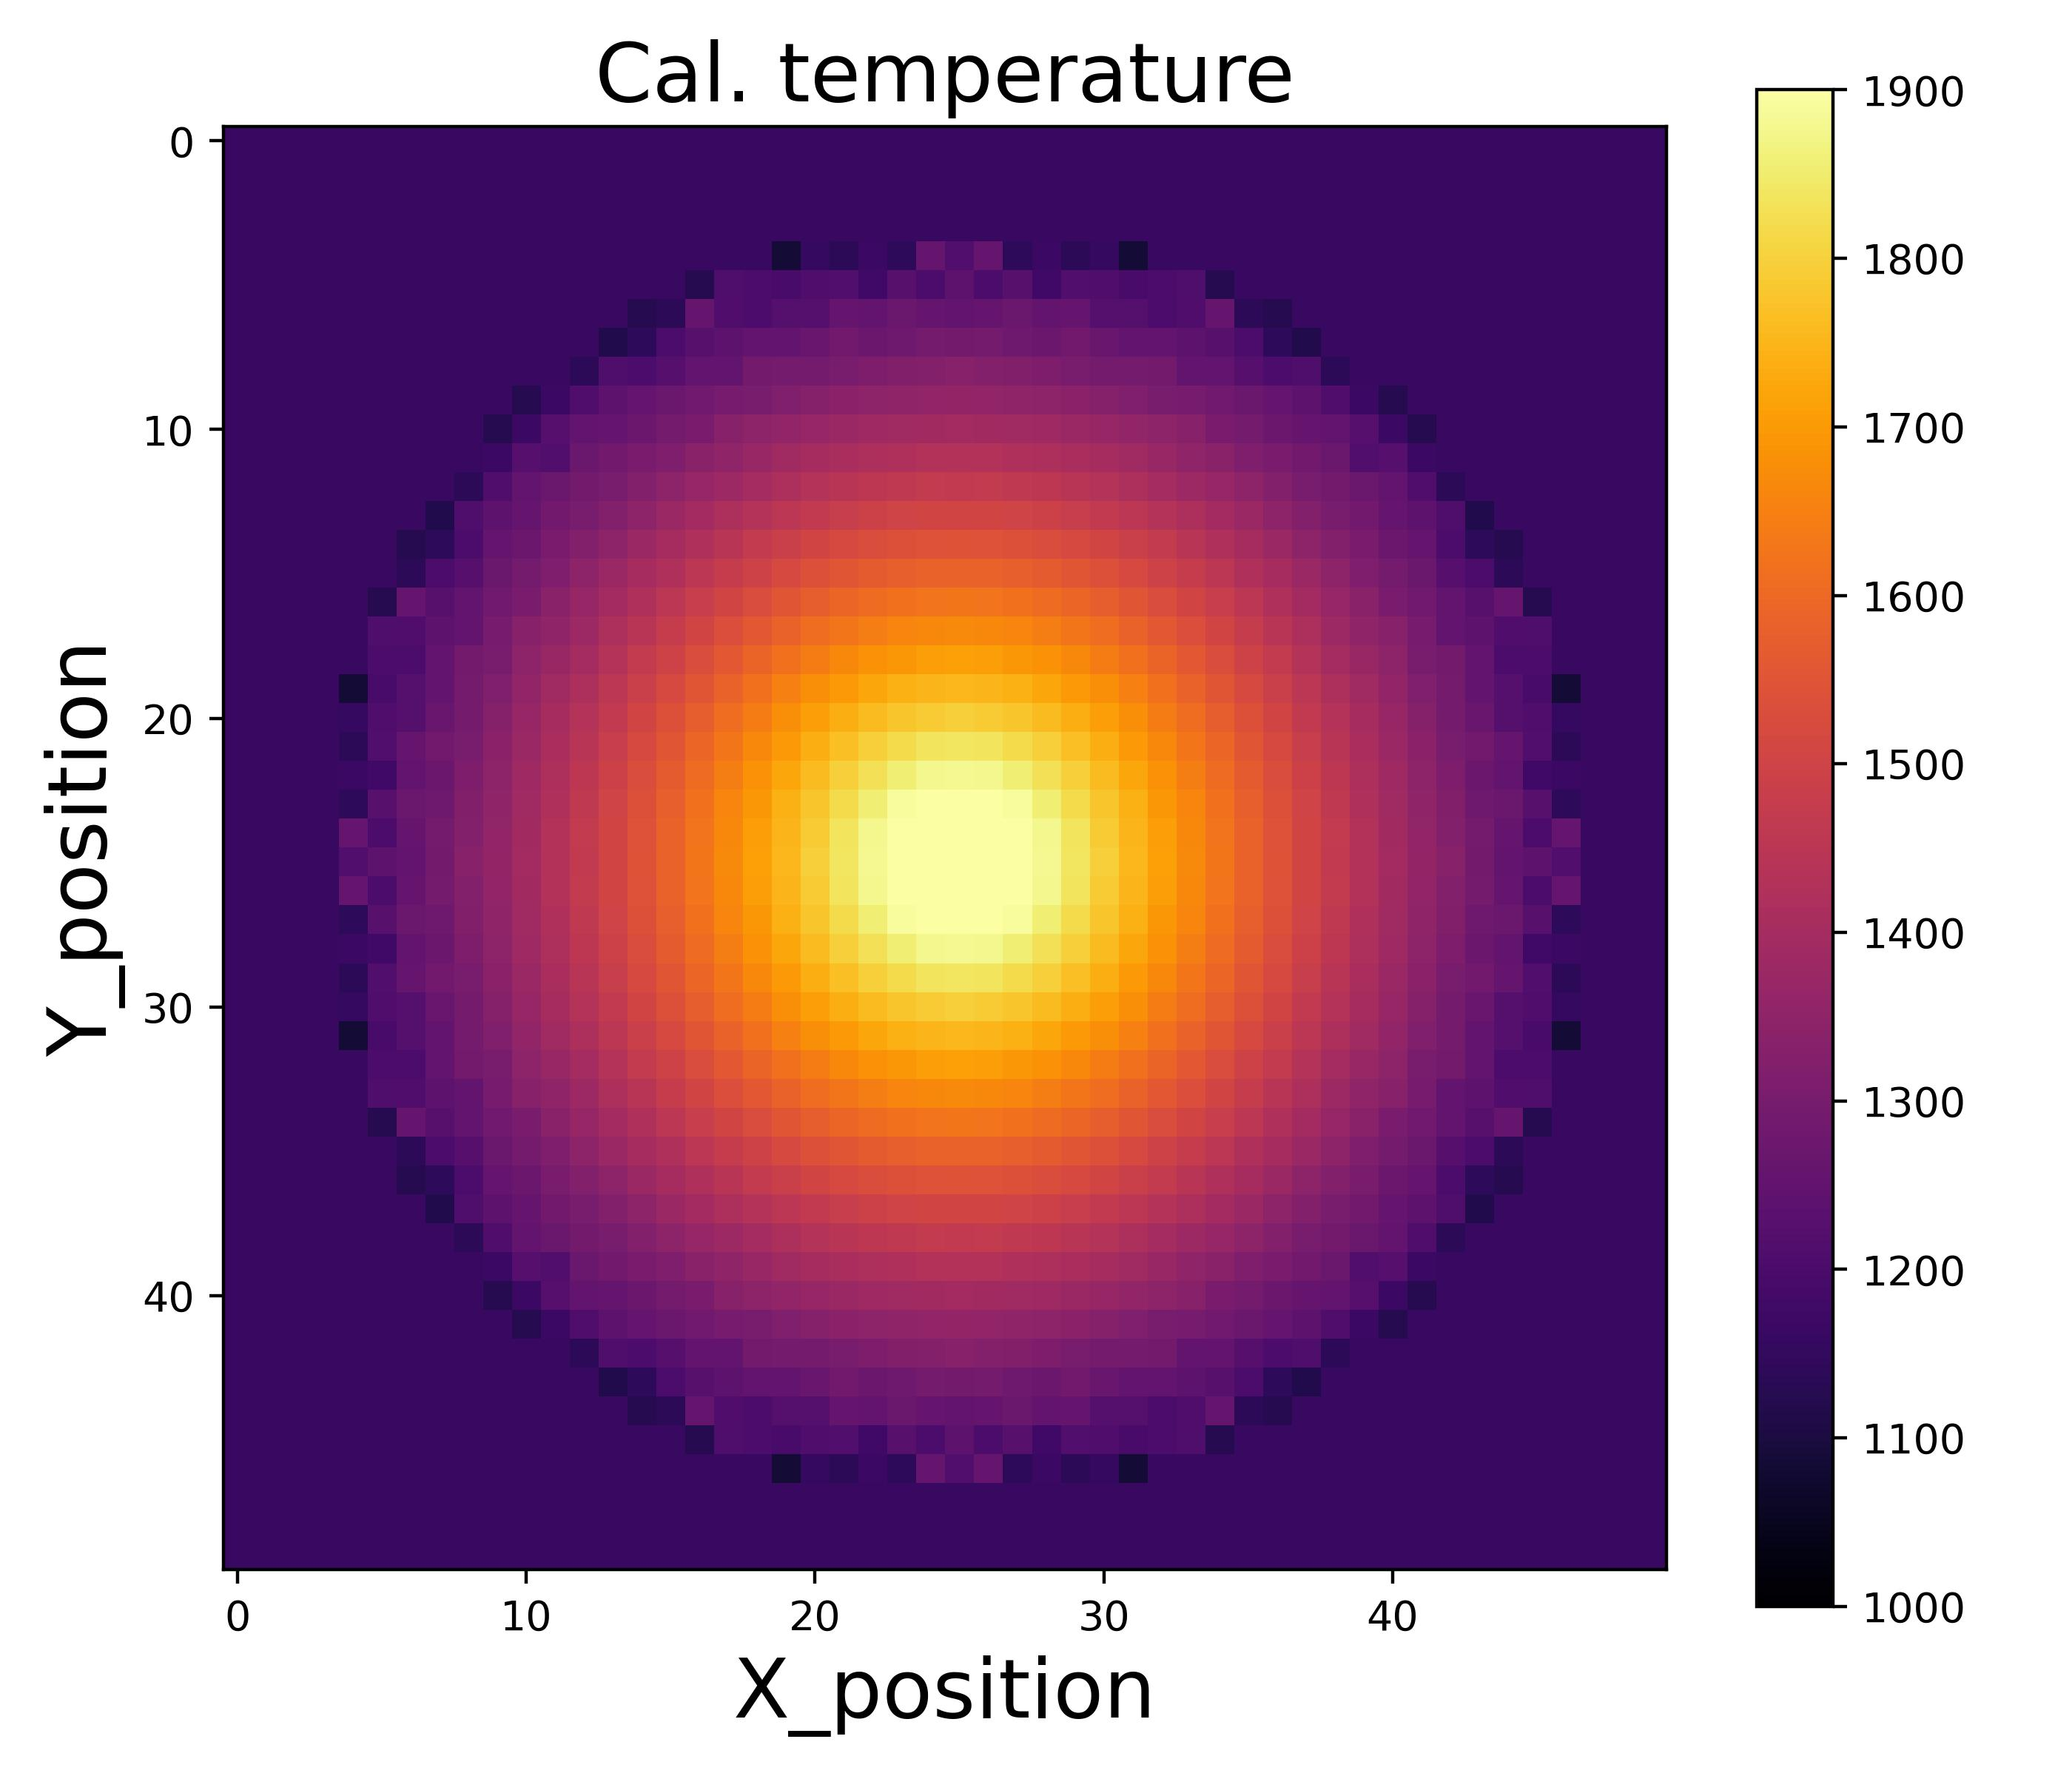
\includegraphics[width=\textwidth]{figures/raw_data/21/lin_square/T_cal.jpg}
        \end{subfigure}
        \begin{subfigure}{0.325\textwidth}
            \centering
            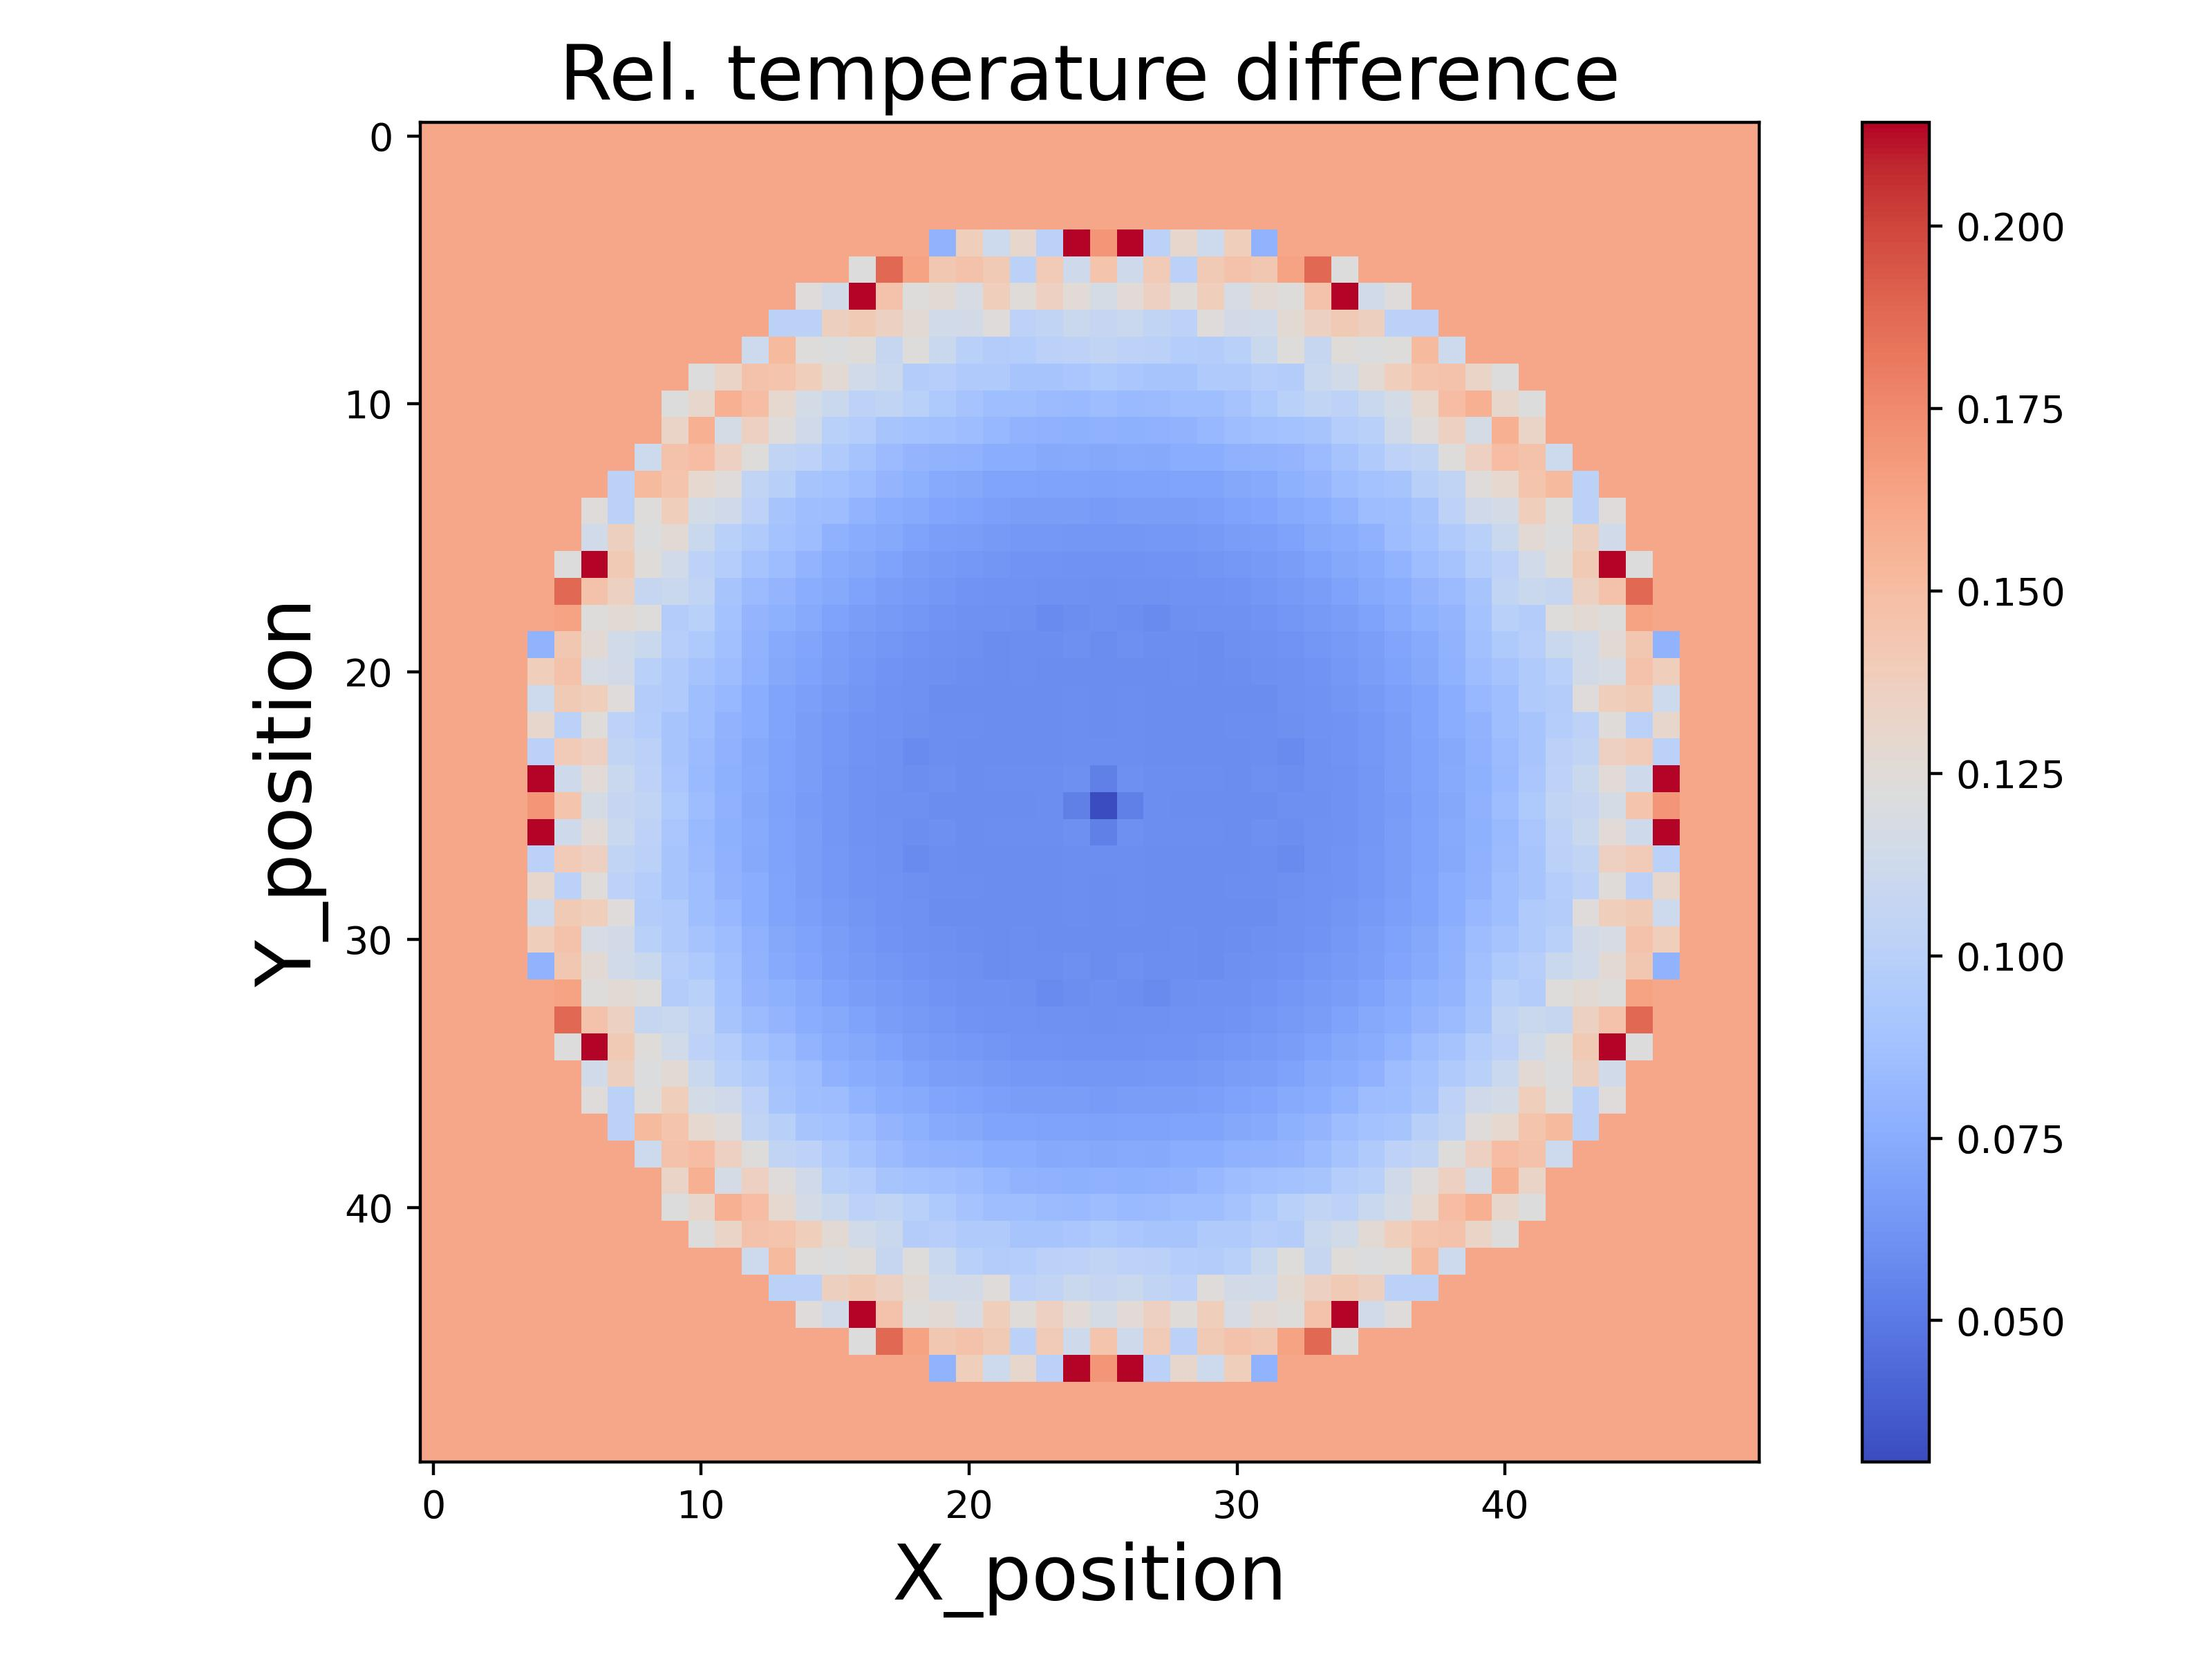
\includegraphics[width=\textwidth]{figures/raw_data/21/lin_square/T_bias.jpg}
        \end{subfigure}
        \begin{subfigure}{0.325\textwidth}
            \centering
            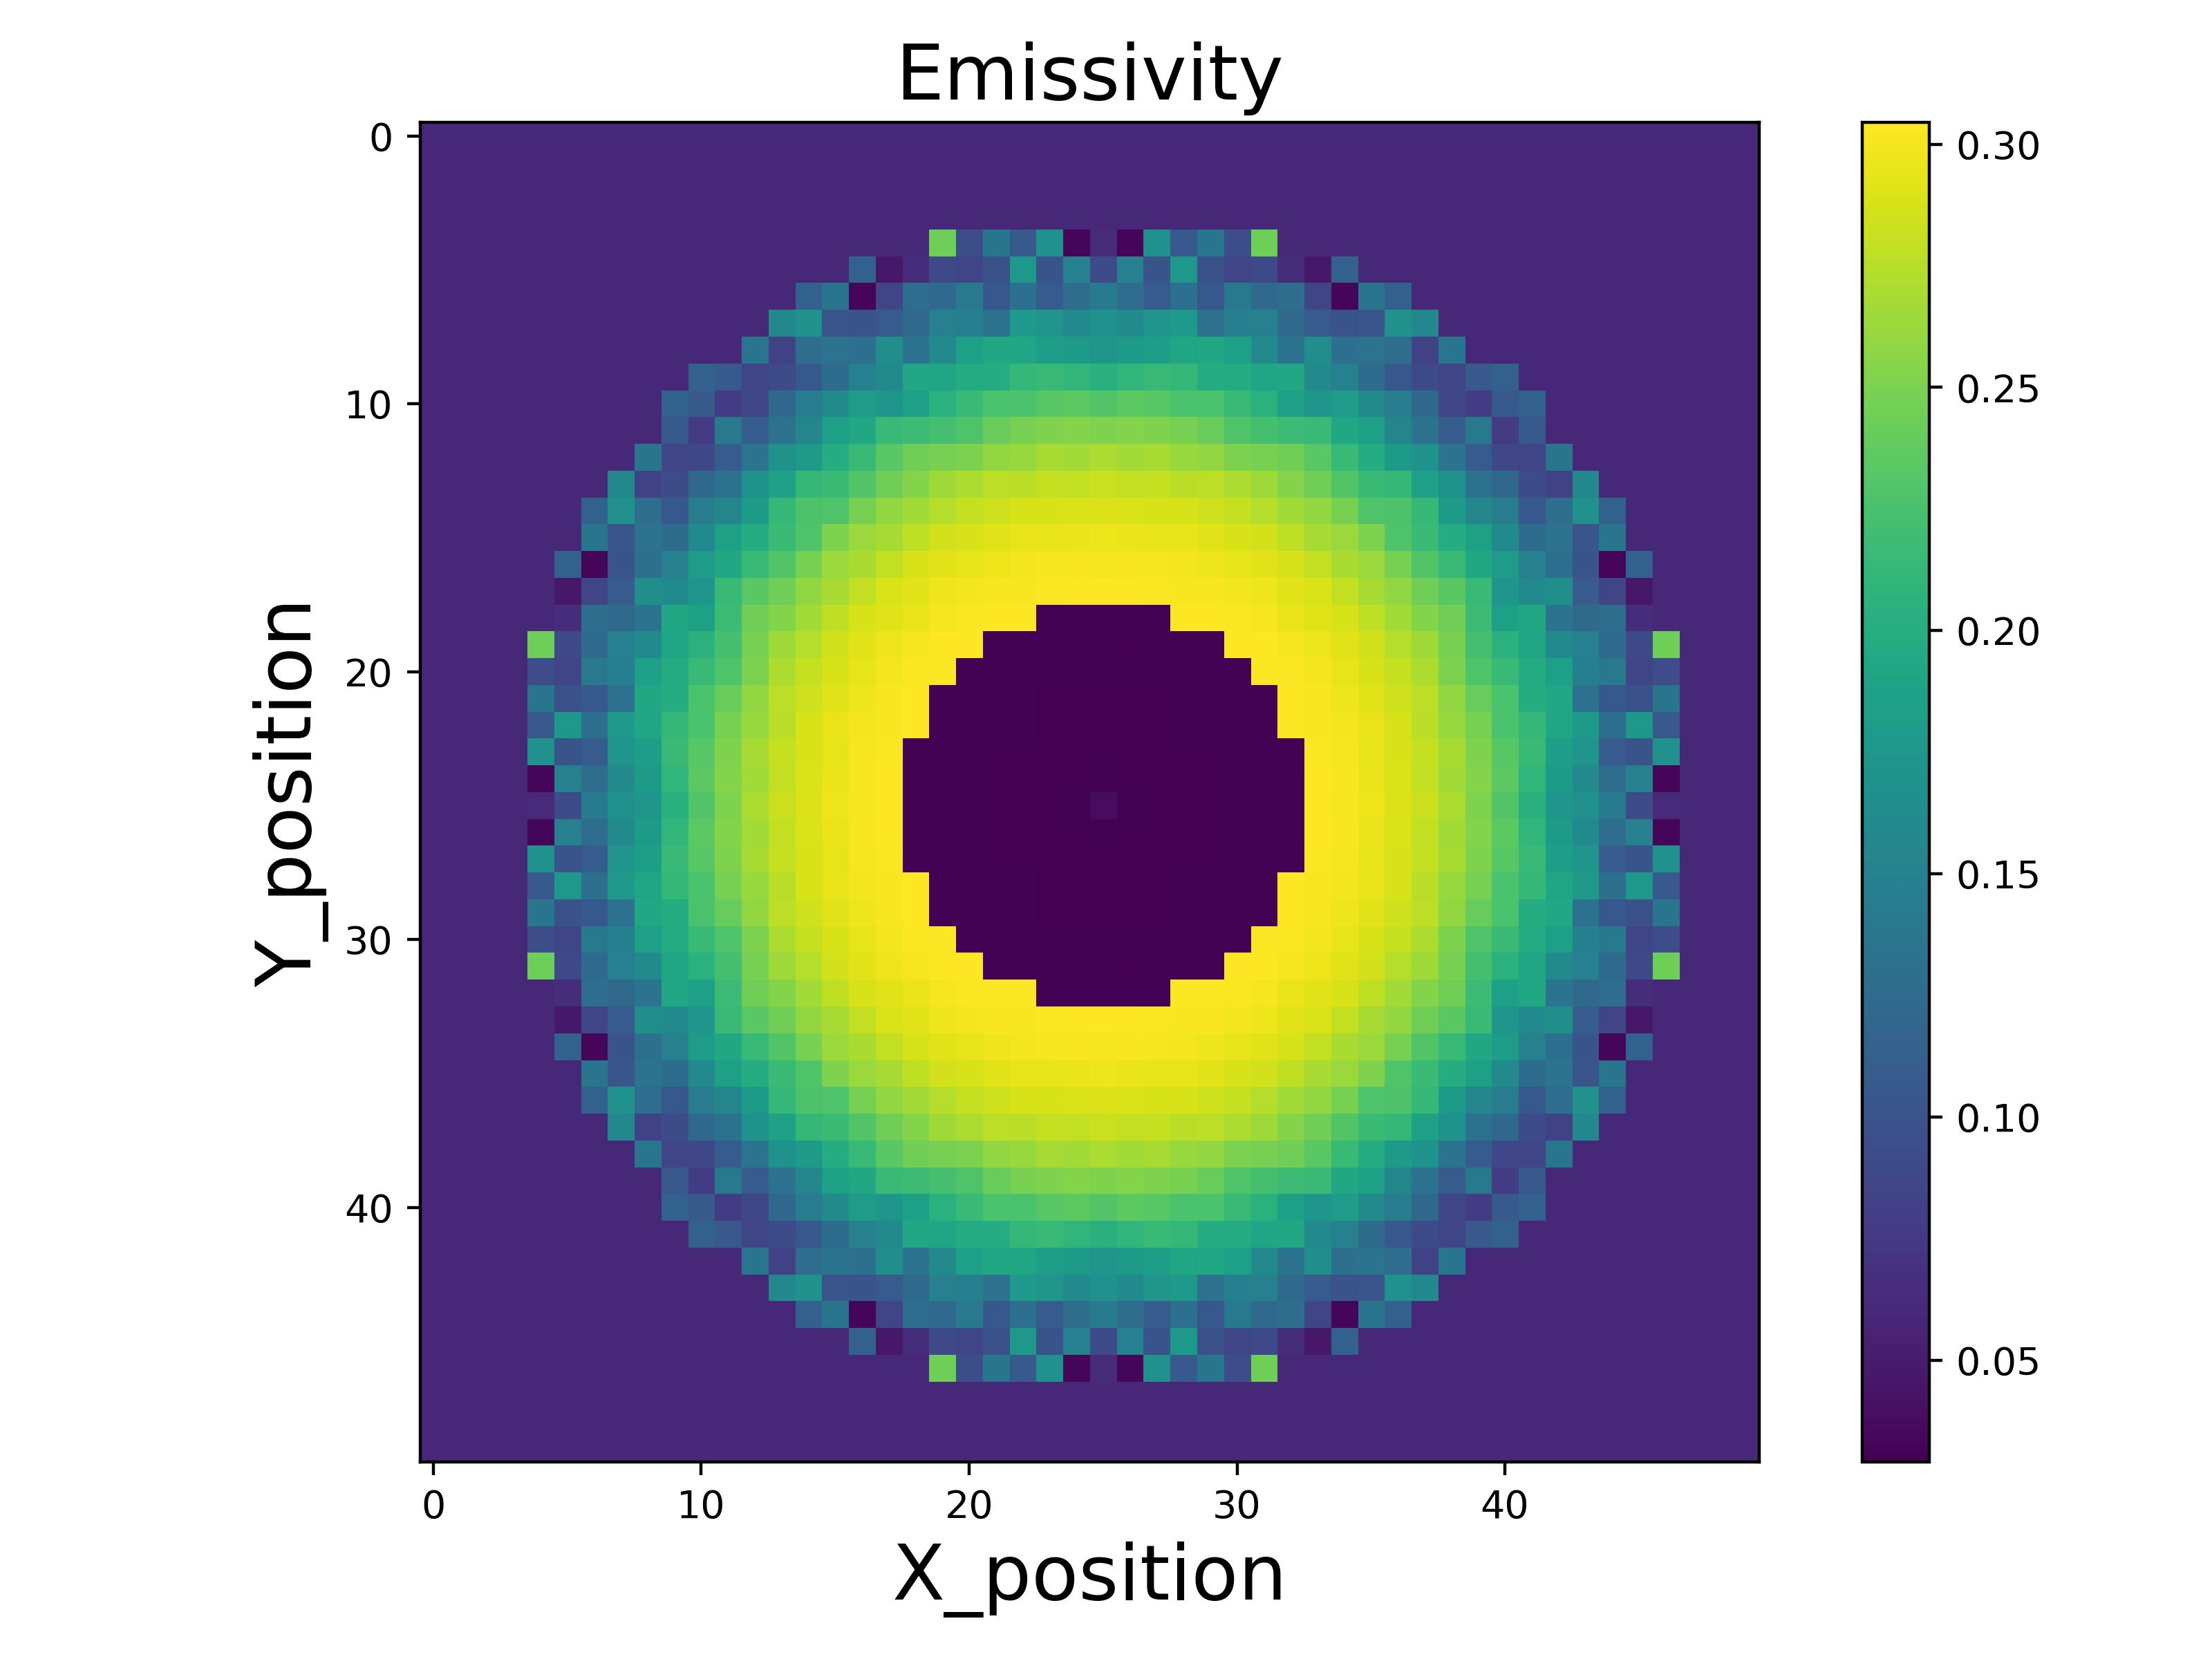
\includegraphics[width=\textwidth]{figures/raw_data/21/lin_square/emi_cal.jpg}
        \end{subfigure}
        \subcaption{Material based on model 1}
    \end{minipage}\\
    \begin{minipage}{\textwidth}
        \centering
        \begin{subfigure}{0.325\textwidth}
            \centering
            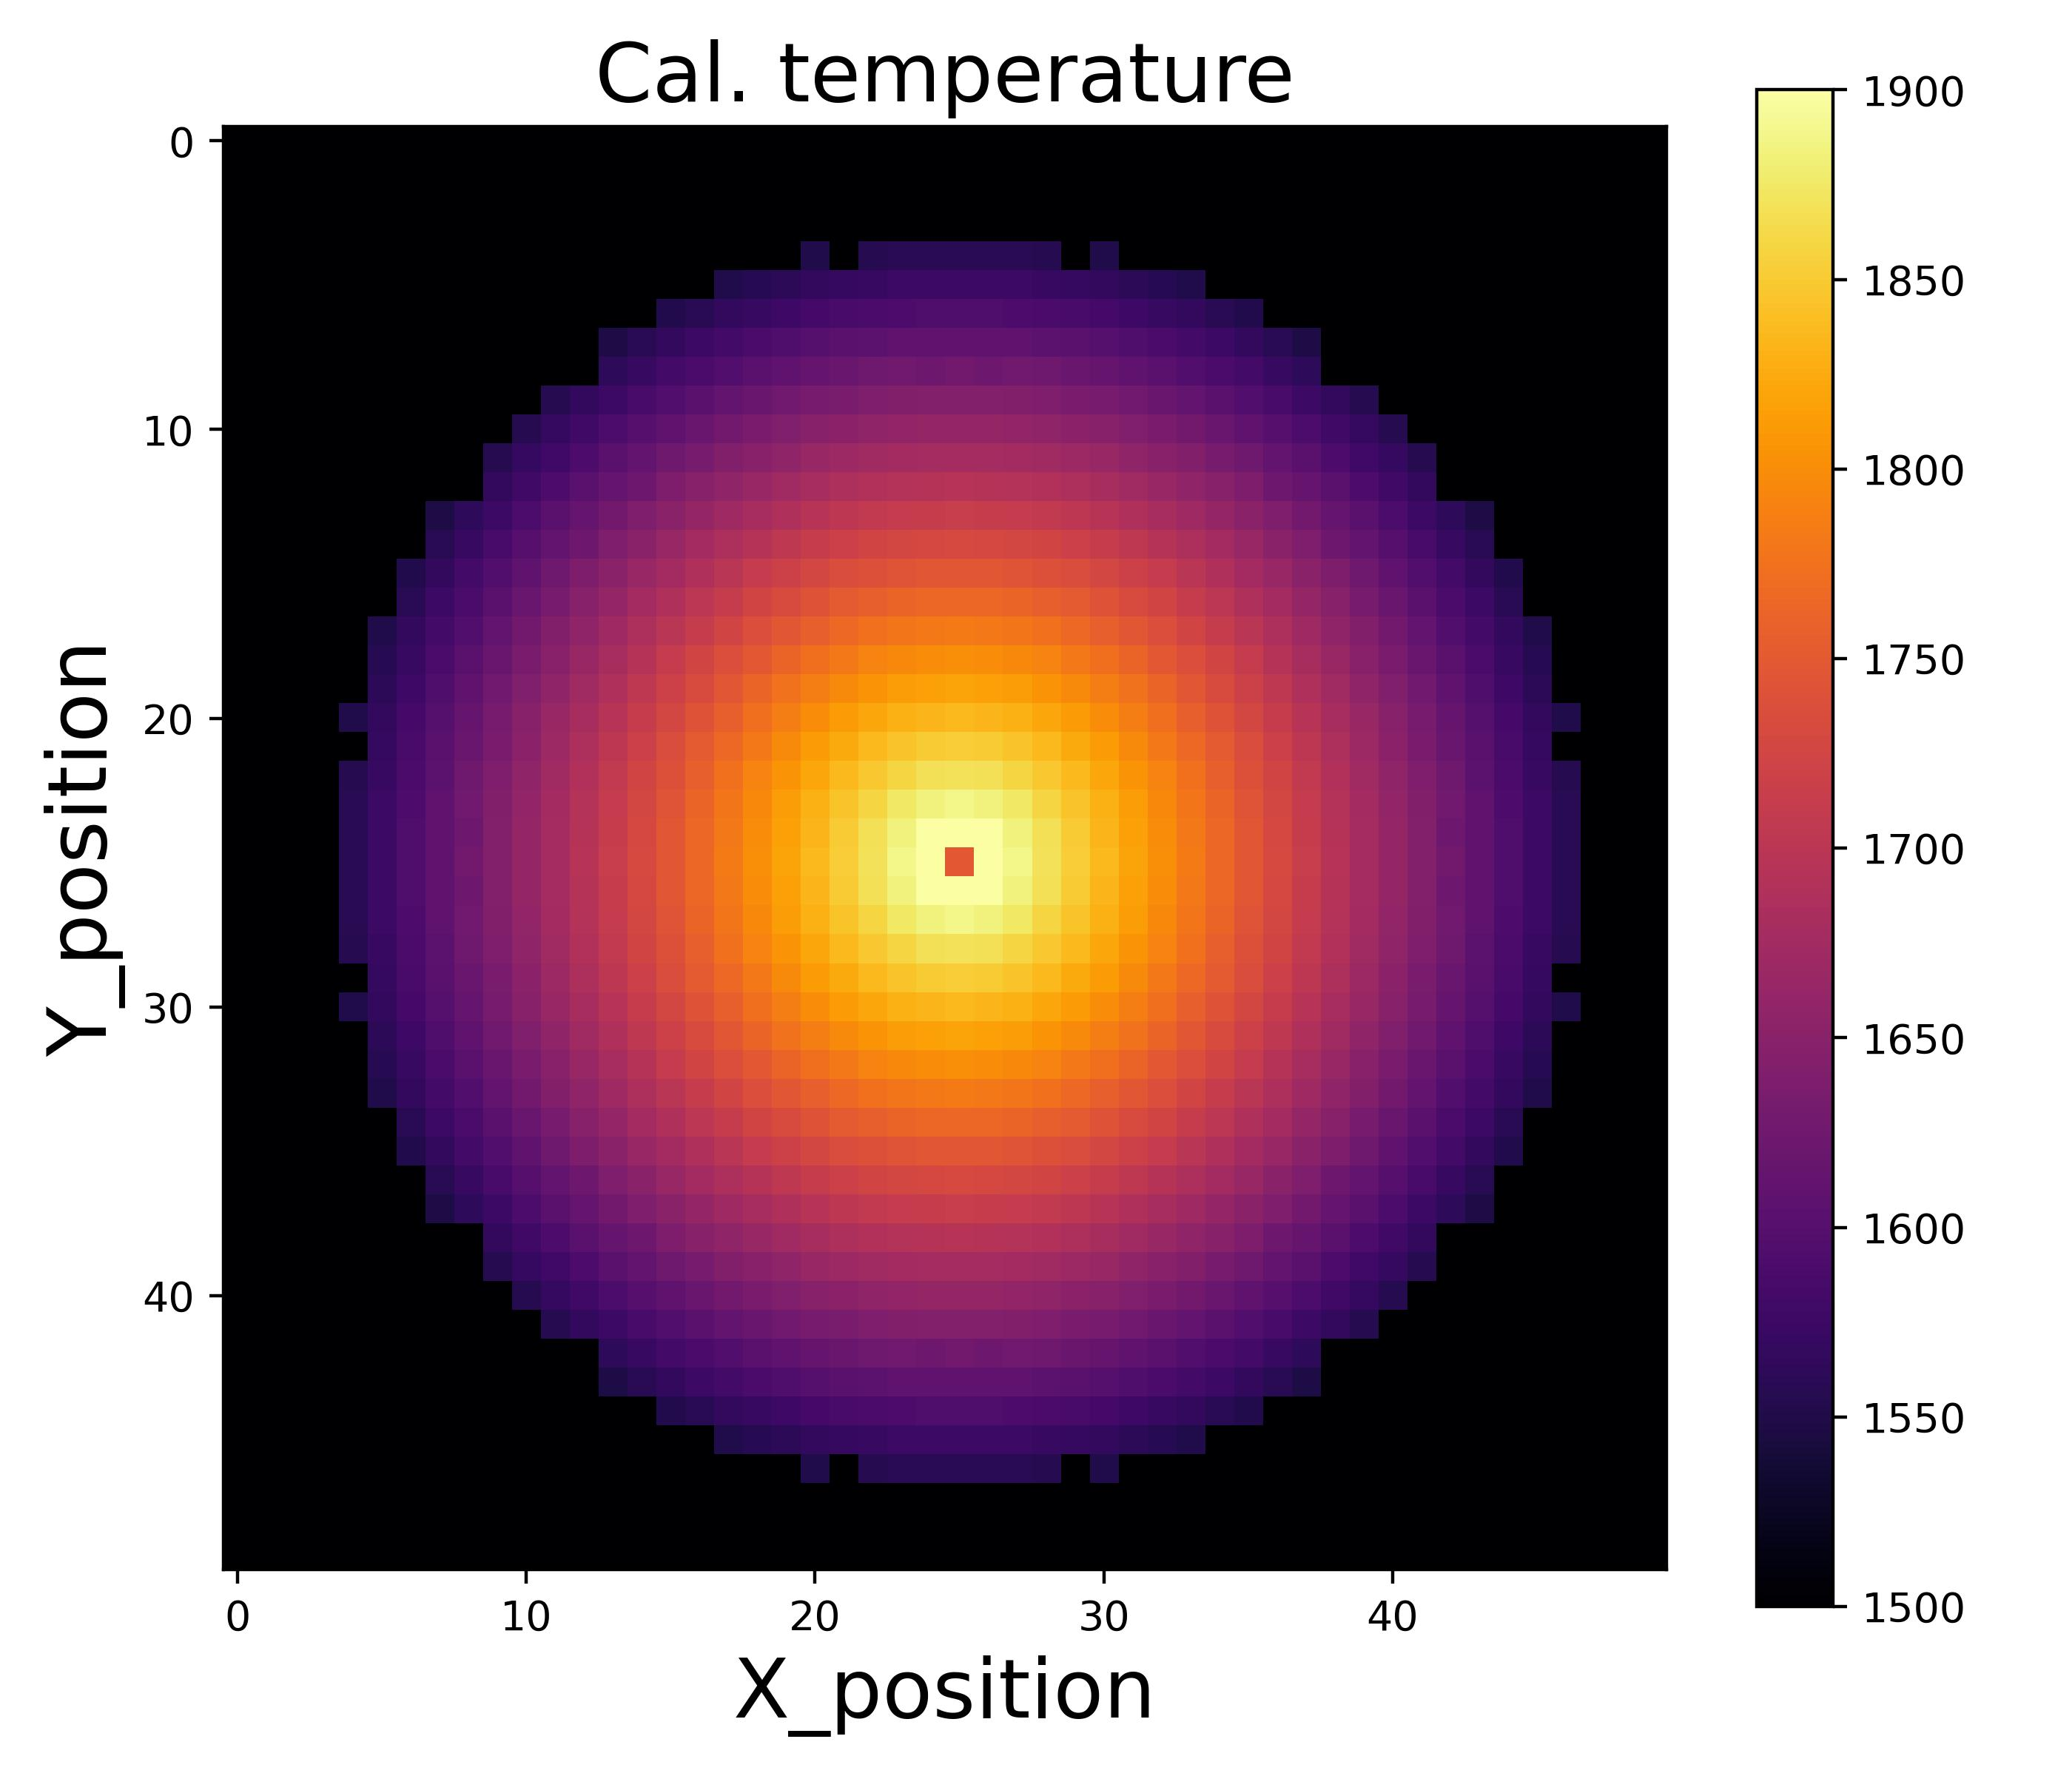
\includegraphics[width=\textwidth]{figures/raw_data/5/lin_square/T_cal.jpg}
        \end{subfigure}
        \begin{subfigure}{0.325\textwidth}
            \centering
            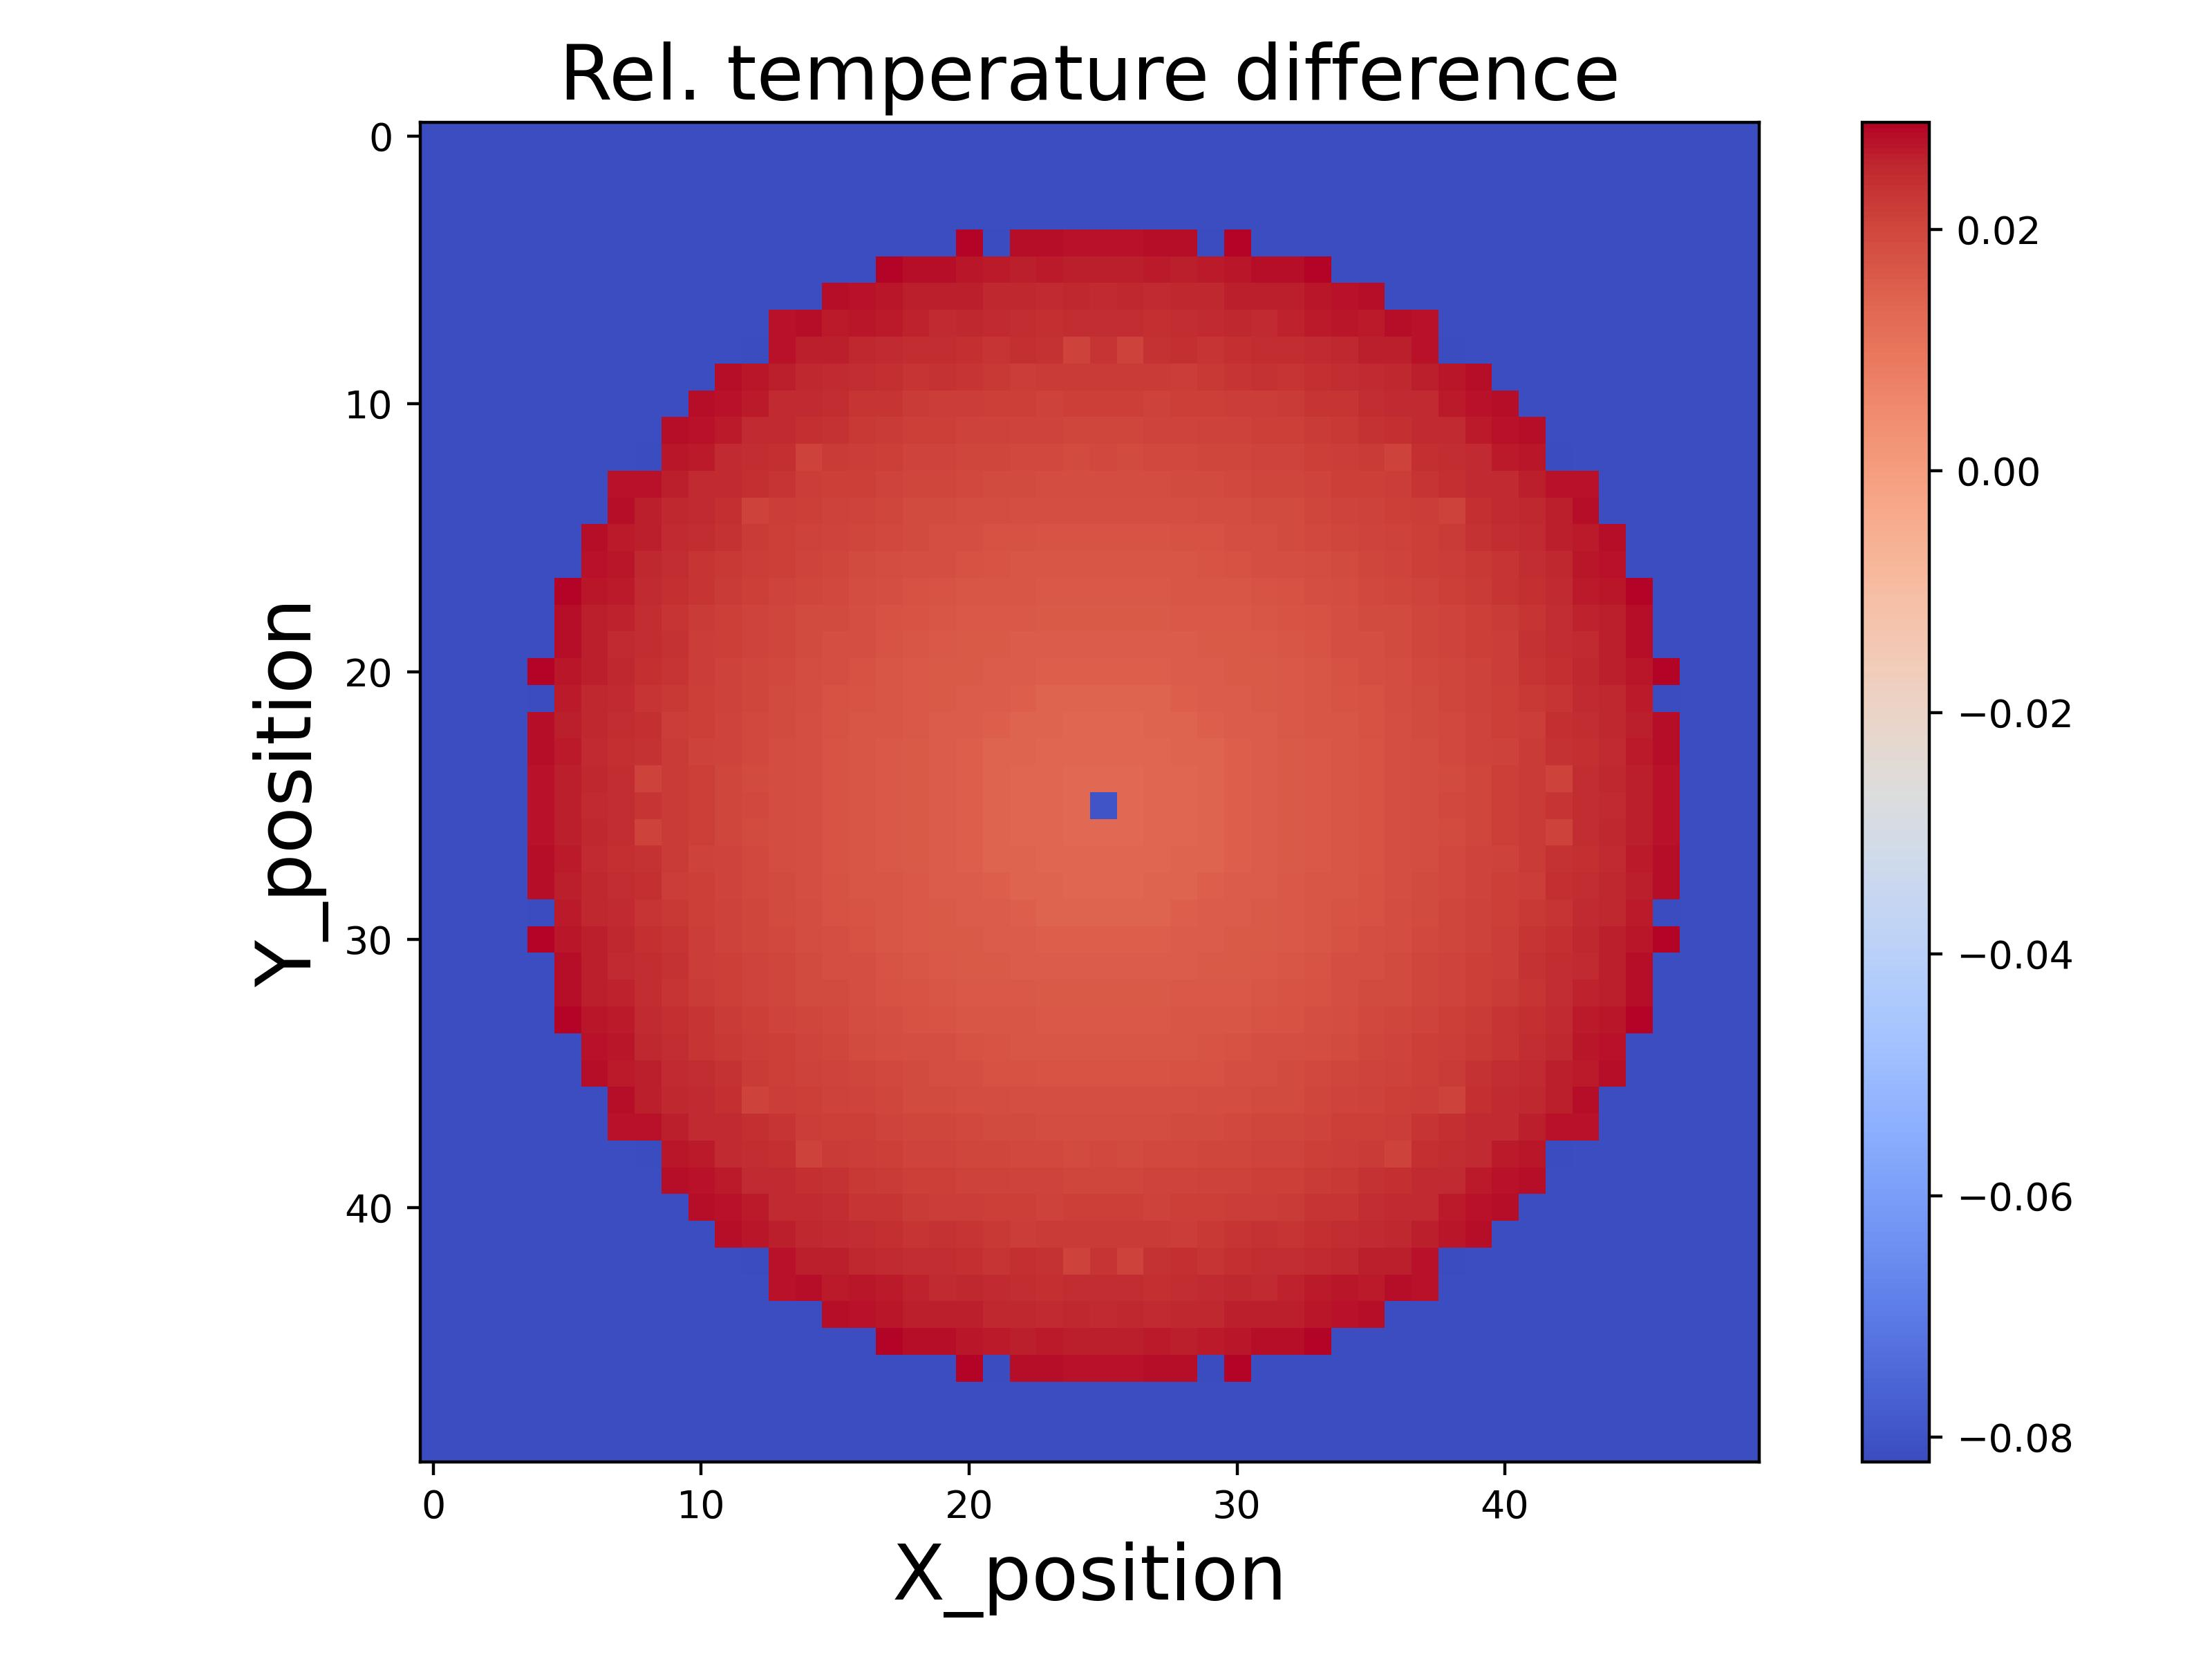
\includegraphics[width=\textwidth]{figures/raw_data/5/lin_square/T_bias.jpg}
        \end{subfigure}
        \begin{subfigure}{0.325\textwidth}
            \centering
            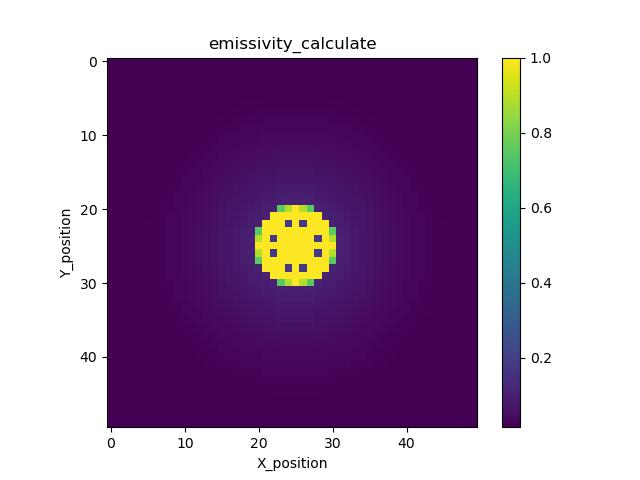
\includegraphics[width=\textwidth]{figures/raw_data/5/lin_square/emi_cal.jpg}
        \end{subfigure}
        \subcaption{Material based on real iron data}
    \end{minipage}
    \caption{Calculation results of linear square model}
    \label{fig: result_linear_square_model}
\end{figure}


Fig.\ref{fig: result_linear_square_model} presents the computational results of the 
linear square model for the virtual experimental data based on both model 1 and 
real iron. It can be observed that the results obtained by the linear square 
model do not exhibit the ring-like pattern that emerges with increasing temperature 
for the hypothetical material. This is because the linear square model possesses 
better capabilities to fit complex emissivity behaviors. In the emissivity plot 
on the right side, it is evident that the linear square model accurately 
reproduces the abrupt change in emissivity in the liquid region without 
causing a significant increase in temperature estimation errors. Thus, it can be 
concluded that the linear square model outperforms the linear model in terms 
of temperature estimation accuracy.


\subsubsection{Quadratic model}

\begin{figure}[htbp]
    \centering
    \begin{minipage}{\textwidth}
        \centering
        \begin{subfigure}{0.325\textwidth}
            \centering
            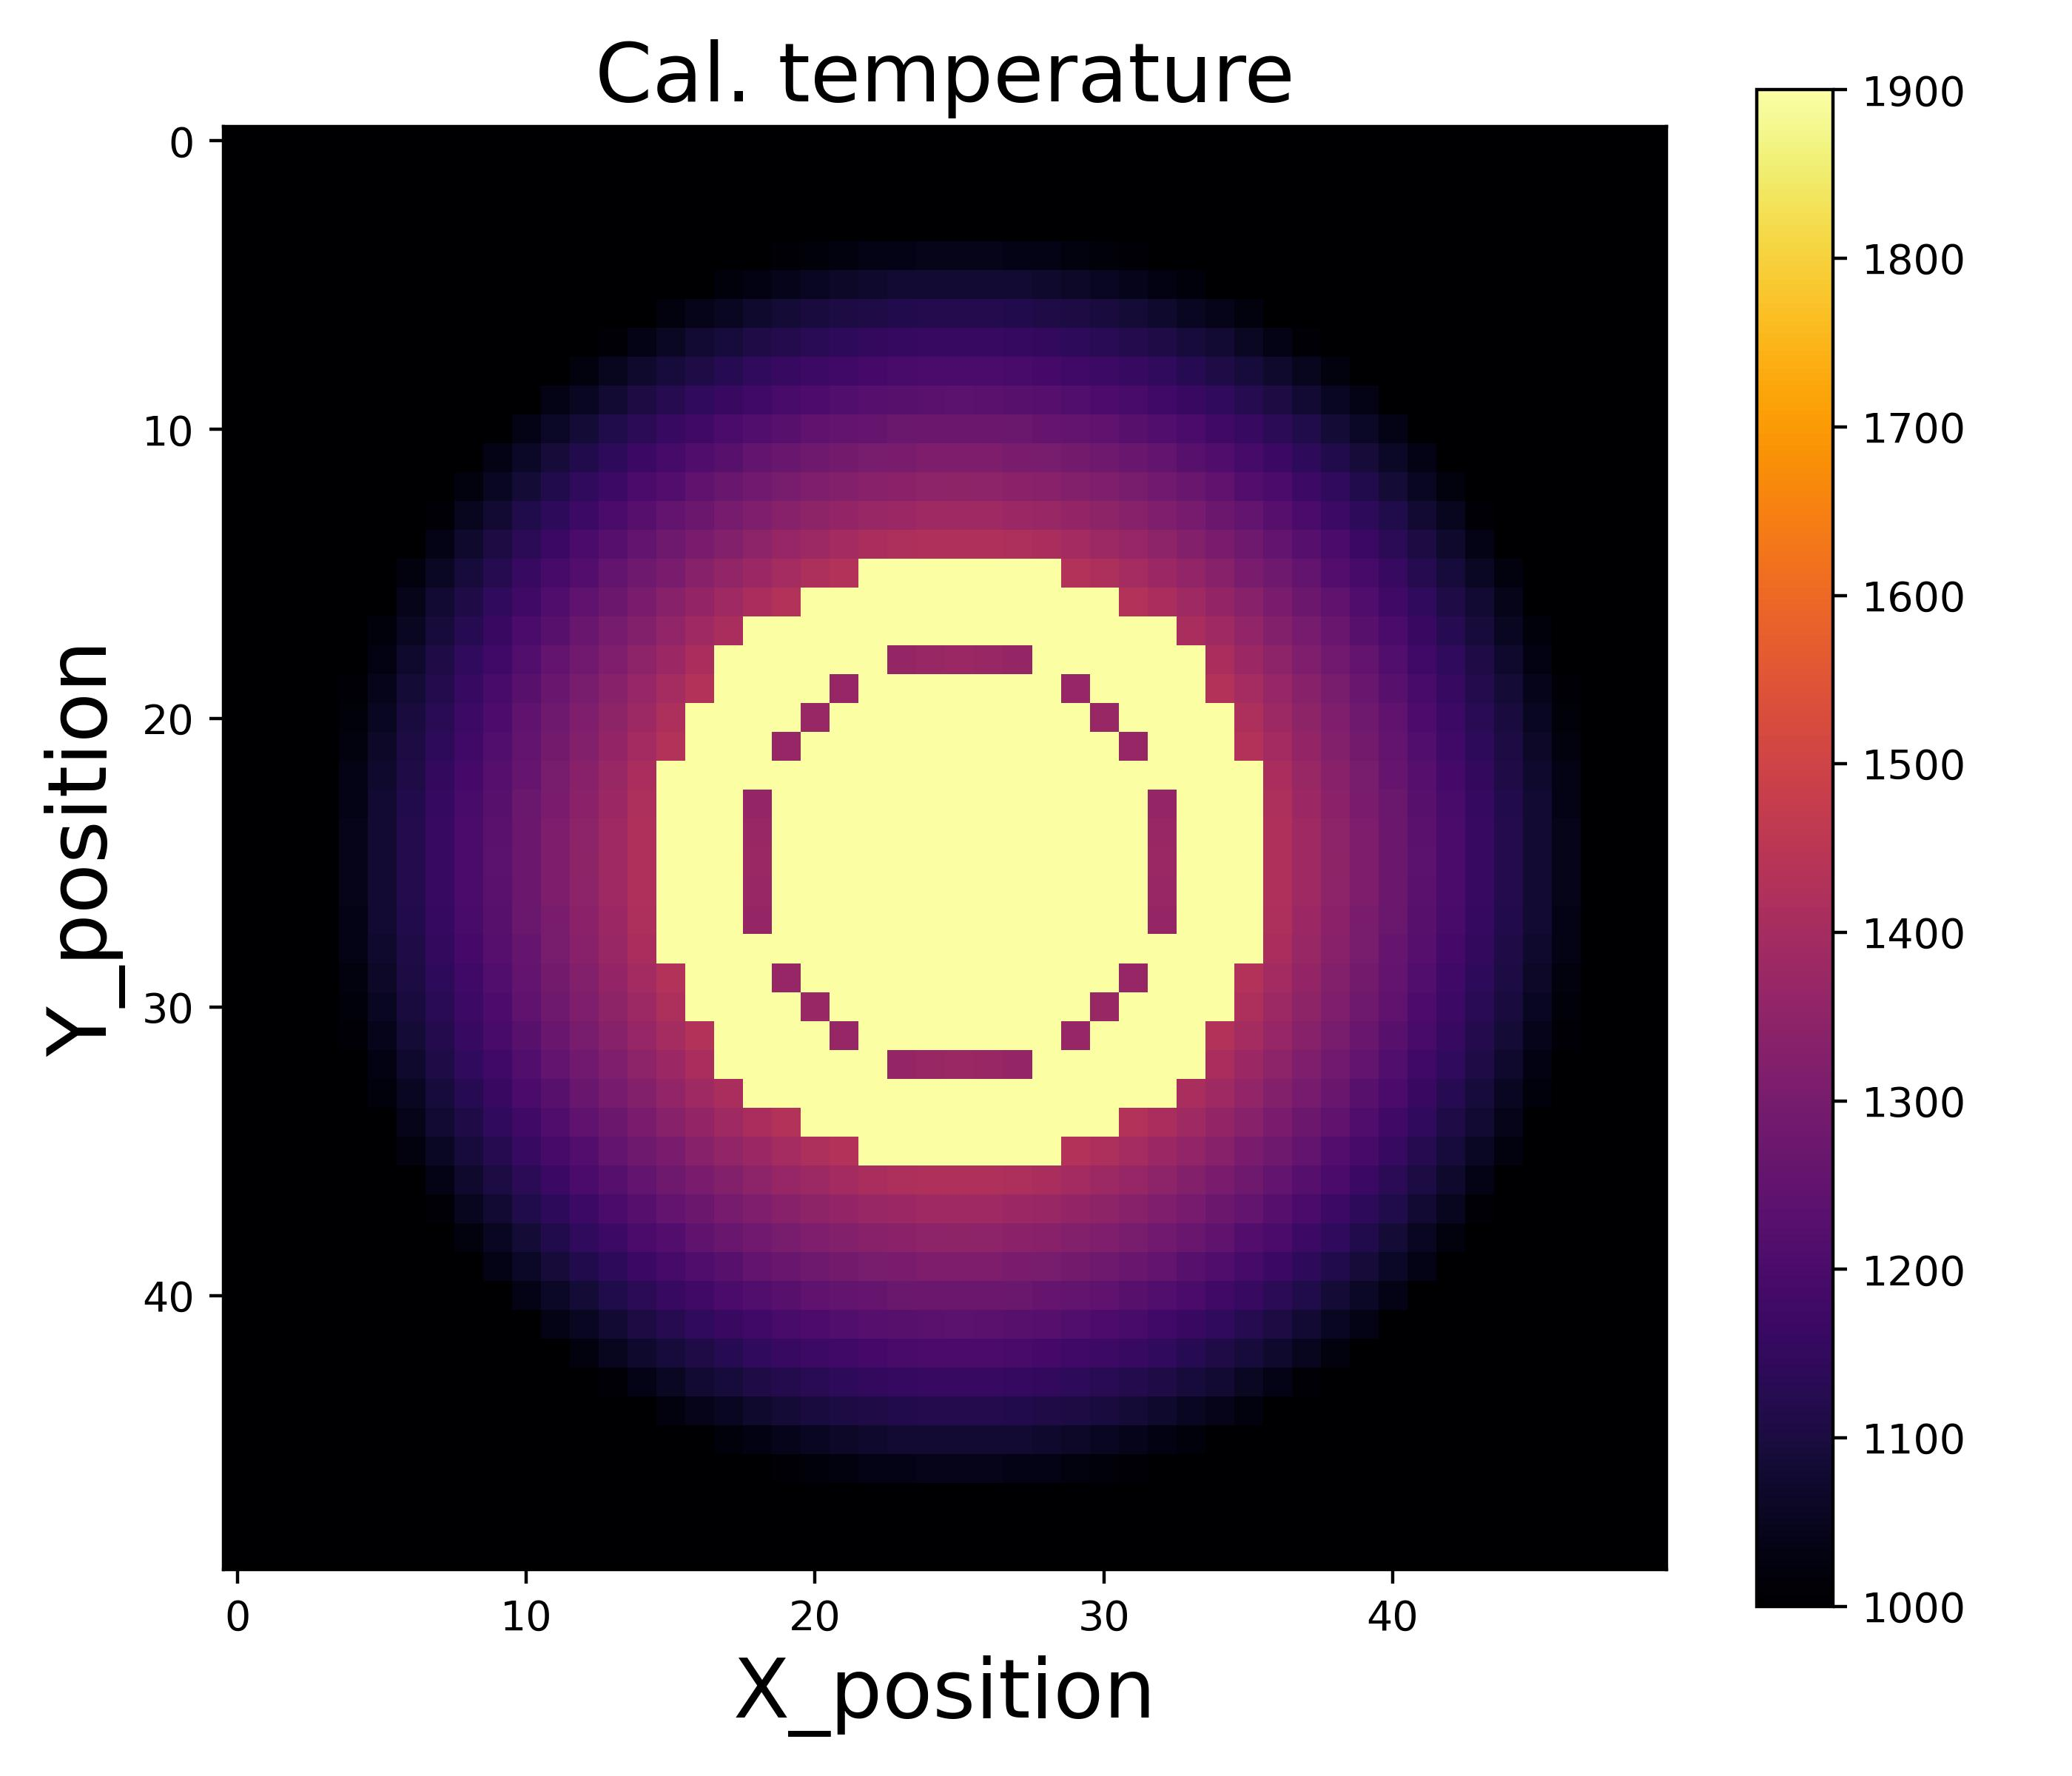
\includegraphics[width=\textwidth]{figures/raw_data/21/quad/T_cal.jpg}
        \end{subfigure}
        \begin{subfigure}{0.325\textwidth}
            \centering
            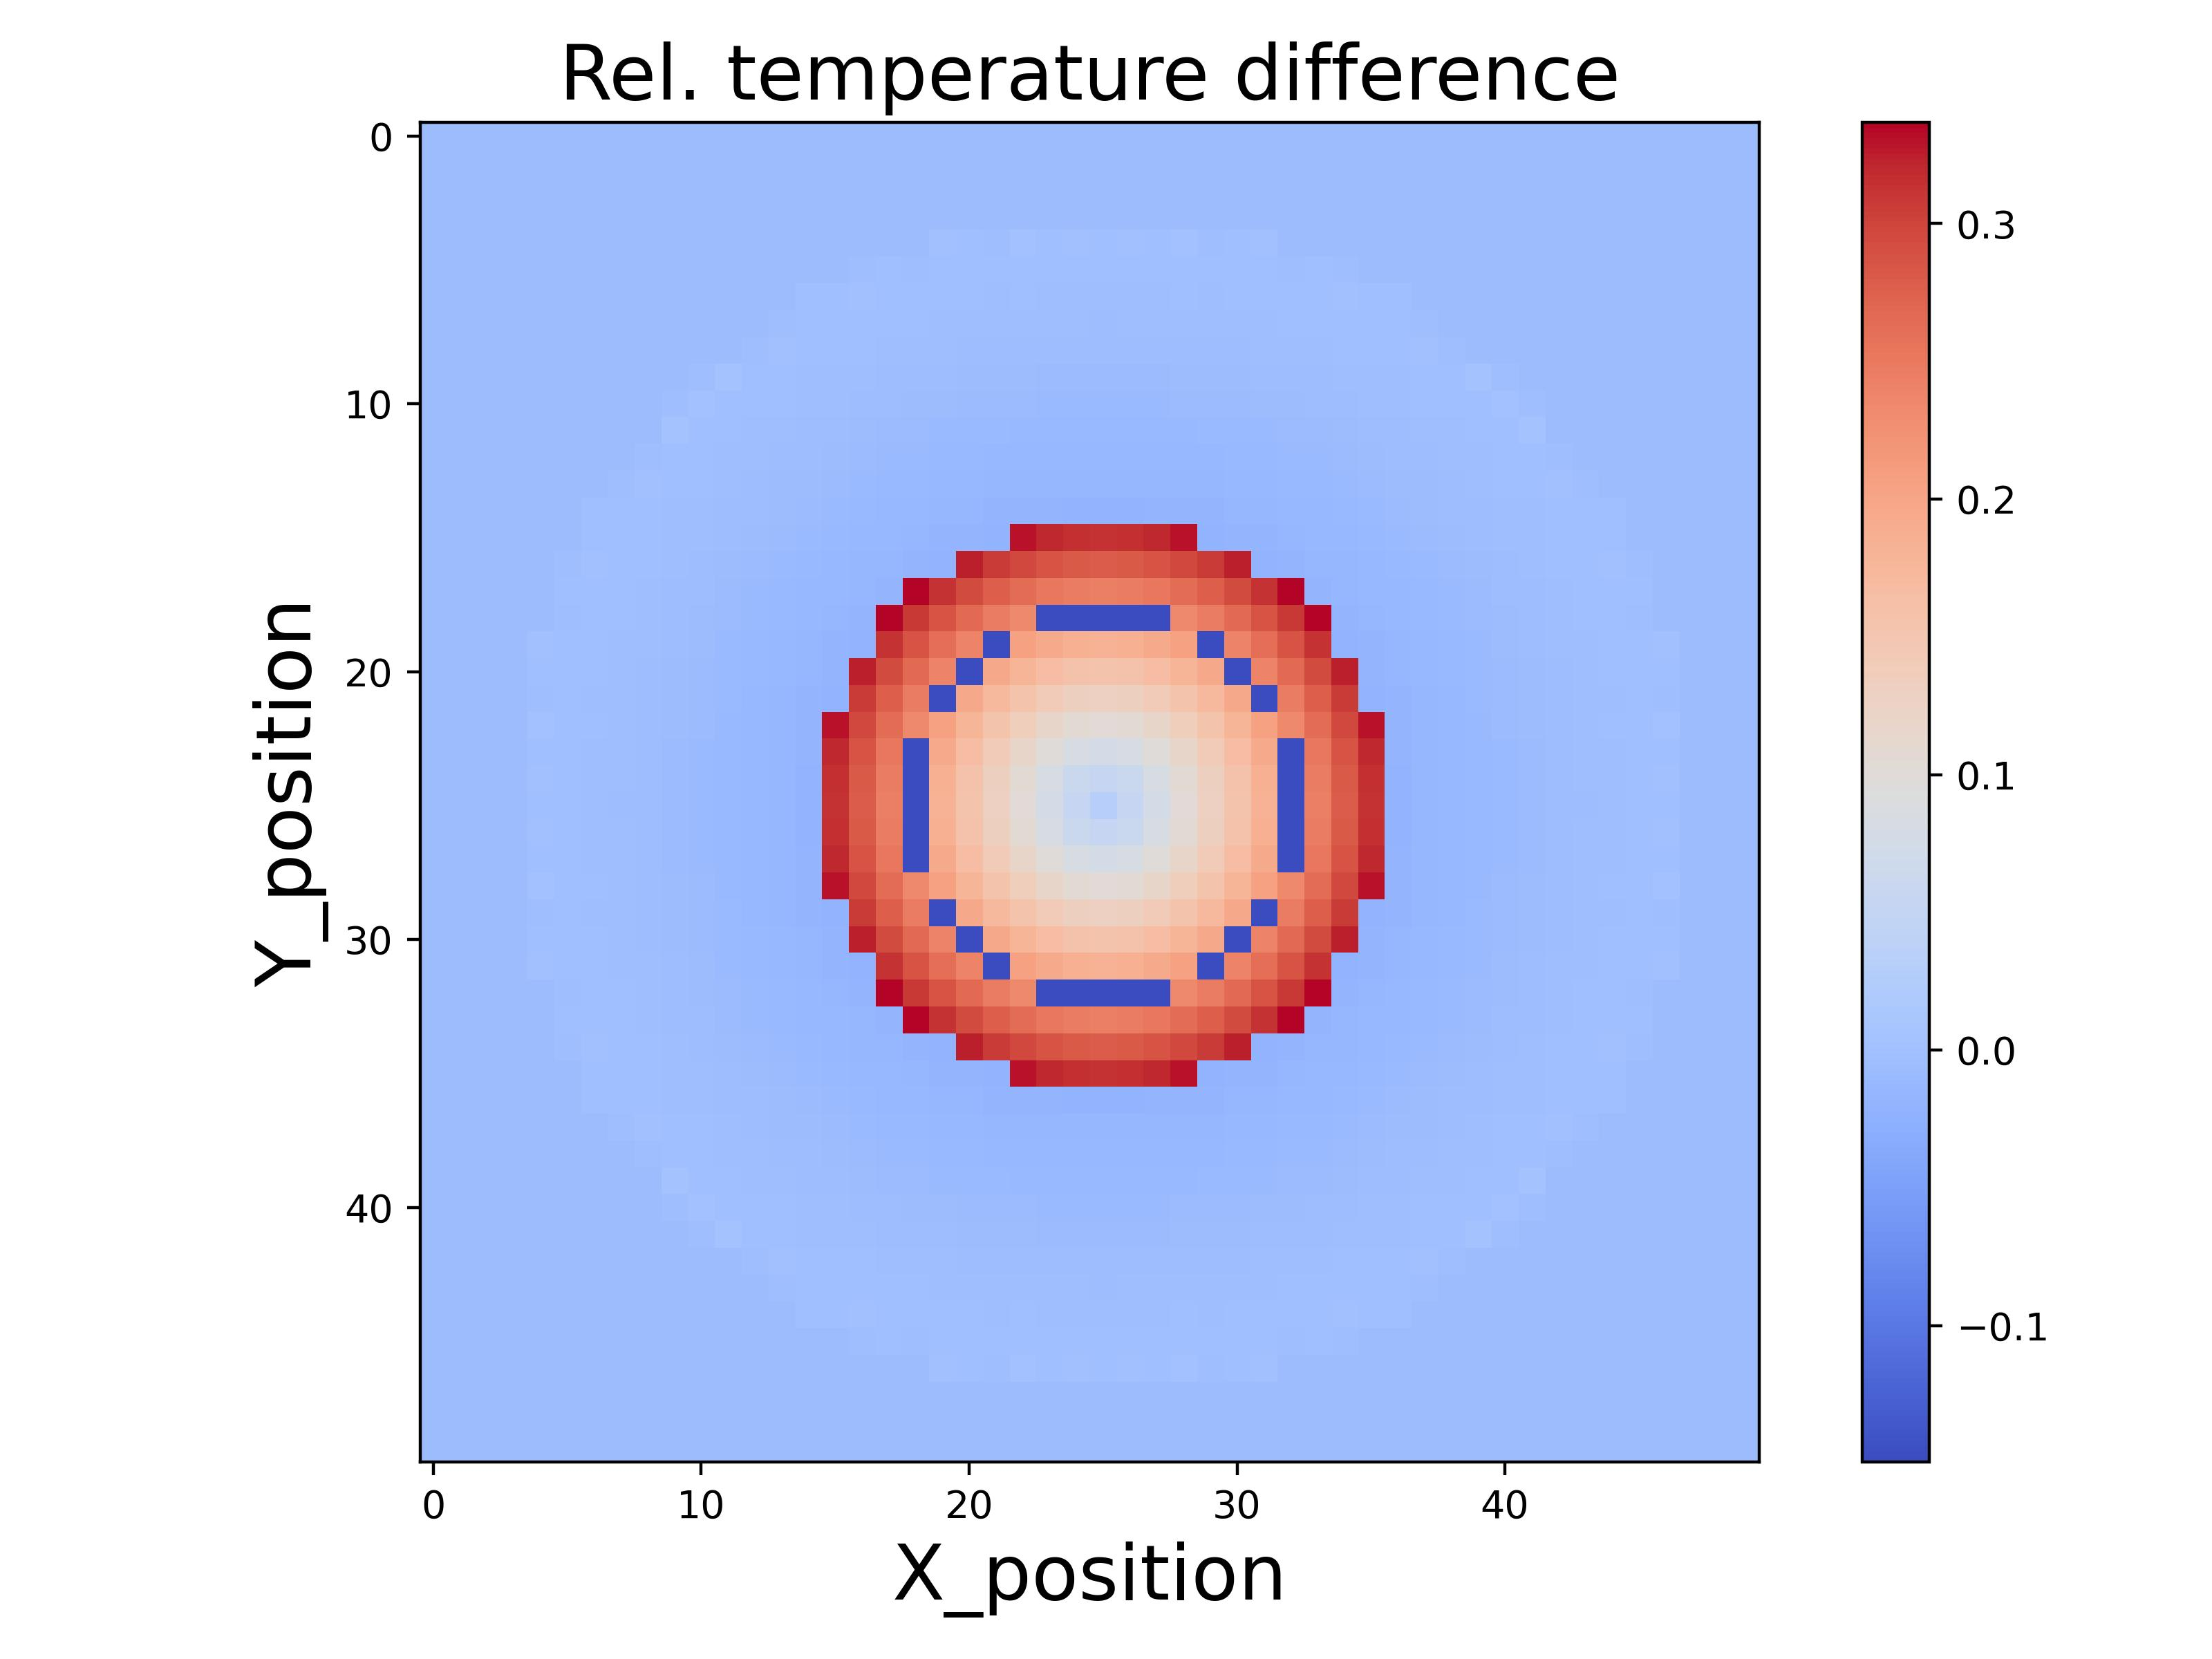
\includegraphics[width=\textwidth]{figures/raw_data/21/quad/T_bias.jpg}
        \end{subfigure}
        \begin{subfigure}{0.325\textwidth}
            \centering
            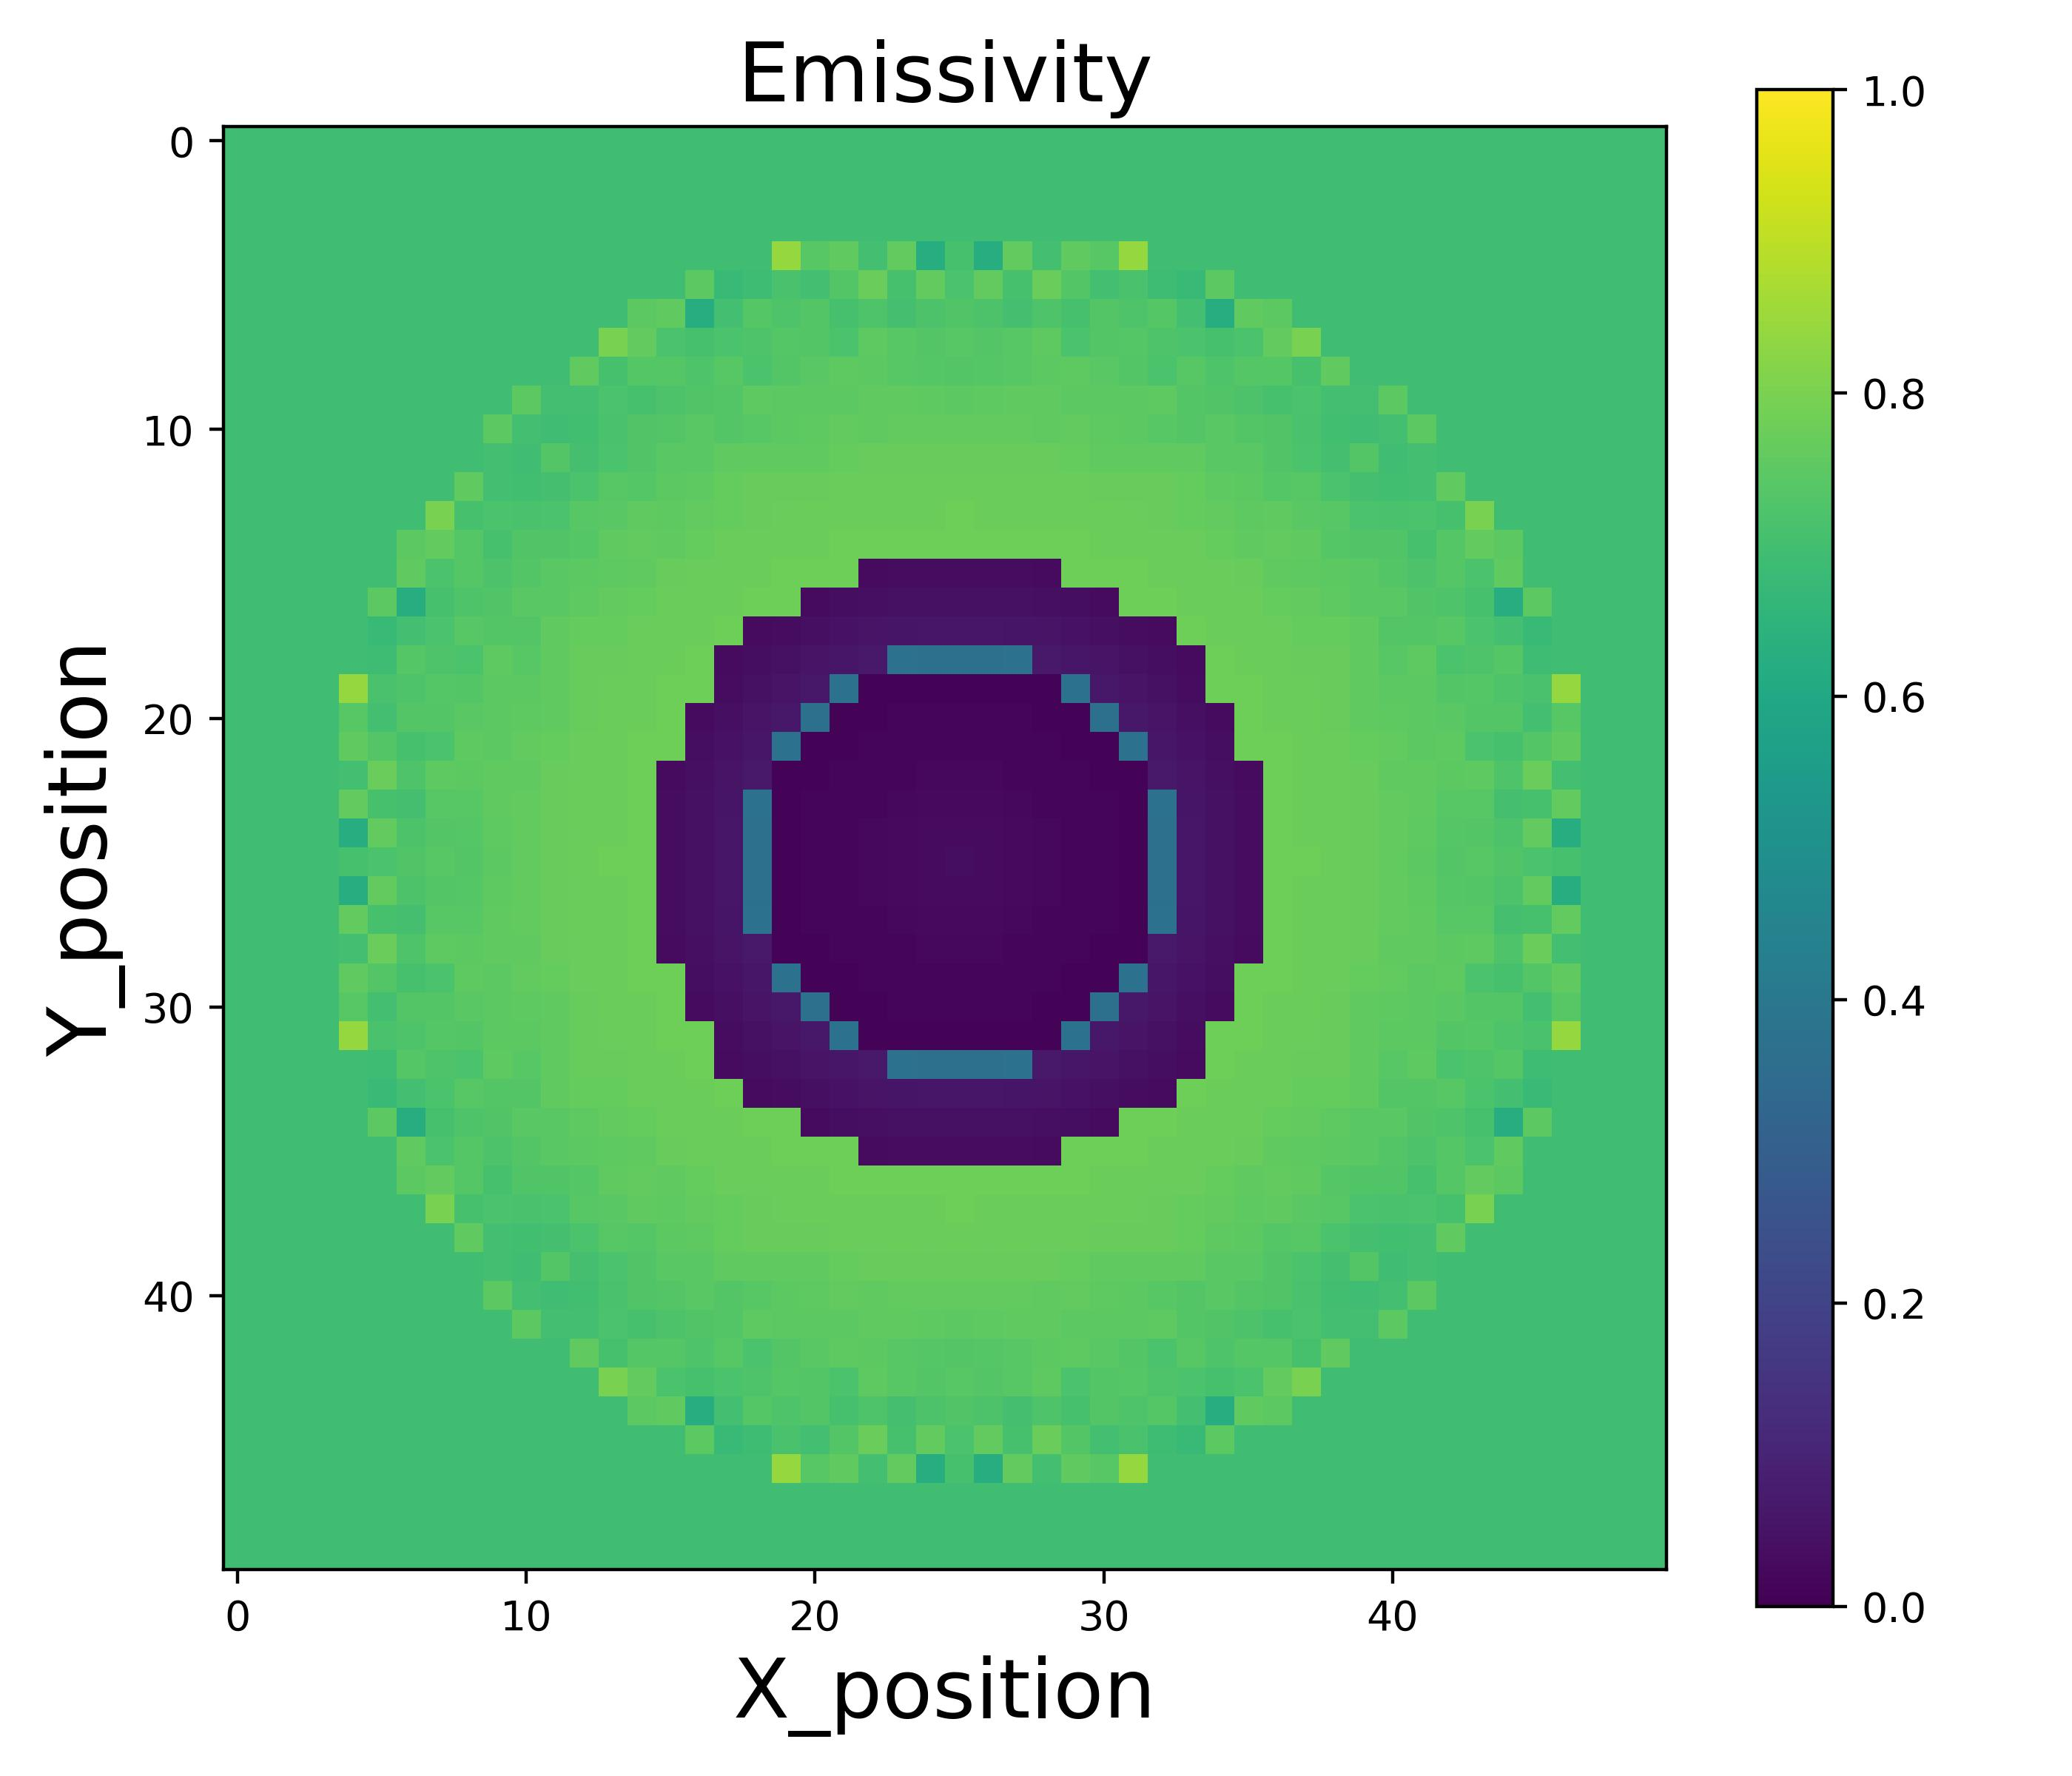
\includegraphics[width=\textwidth]{figures/raw_data/21/quad/emi_cal.jpg}
        \end{subfigure}
        \subcaption{Material based on model 1}
    \end{minipage}\\
    \begin{minipage}{\textwidth}
        \centering
        \begin{subfigure}{0.325\textwidth}
            \centering
            \includegraphics[width=\textwidth]{figures/raw_data/5/quad/T_cal.jpg}
        \end{subfigure}
        \begin{subfigure}{0.325\textwidth}
            \centering
            \includegraphics[width=\textwidth]{figures/raw_data/5/quad/T_bias.jpg}
        \end{subfigure}
        \begin{subfigure}{0.325\textwidth}
            \centering
            \includegraphics[width=\textwidth]{figures/raw_data/5/quad/emi_cal.jpg}
        \end{subfigure}
        \subcaption{Material based on real iron data}
    \end{minipage}
    \caption{Calculation results of quadratic model}
    \label{fig: result_quadratic_model}
\end{figure}


Unlike the previously mentioned linear square model, the quadratic model has one 
fewer parameter, resulting in fewer degrees of freedom for the emissivity model. 
In fact, based on Eq.\ref{eq: emi_quad} from the paper, this mathematical 
model ss y-axis symmetry. Considering the physical meaning of emissivity, 
it can only be used to fit emissivity models that are either monotonically 
increasing or monotonically decreasing.

As a result, as shown in Fig.\ref{fig: result_quadratic_model}, it can be observed 
that in the computations based on model 1 for the material, the performance 
of the temperature estimation algorithm is better at the central point 
(the location with the highest temperature) compared to other regions due to less 
variations in emissivity.
The results of the emissivity field demonstrate that the algorithm accurately 
identifies the boundary regions between liquid and solid materials.

However, for computations involving real materials, the algorithm struggles to 
accurately estimate the emissivity of hypothetical materials, leading to errors in 
temperature calculations. Nevertheless, it is still evident that the 
temperature estimation algorithm based on the quadratic model performs better 
on real materials compared to hypothetical materials.

\subsubsection{Exponential model}

\begin{figure}[htbp]
    \centering
    \begin{minipage}{\textwidth}
        \centering
        \begin{subfigure}{0.325\textwidth}
            \centering
            \includegraphics[width=\textwidth]{figures/raw_data/21/exp/T_cal.jpg}
        \end{subfigure}
        \begin{subfigure}{0.325\textwidth}
            \centering
            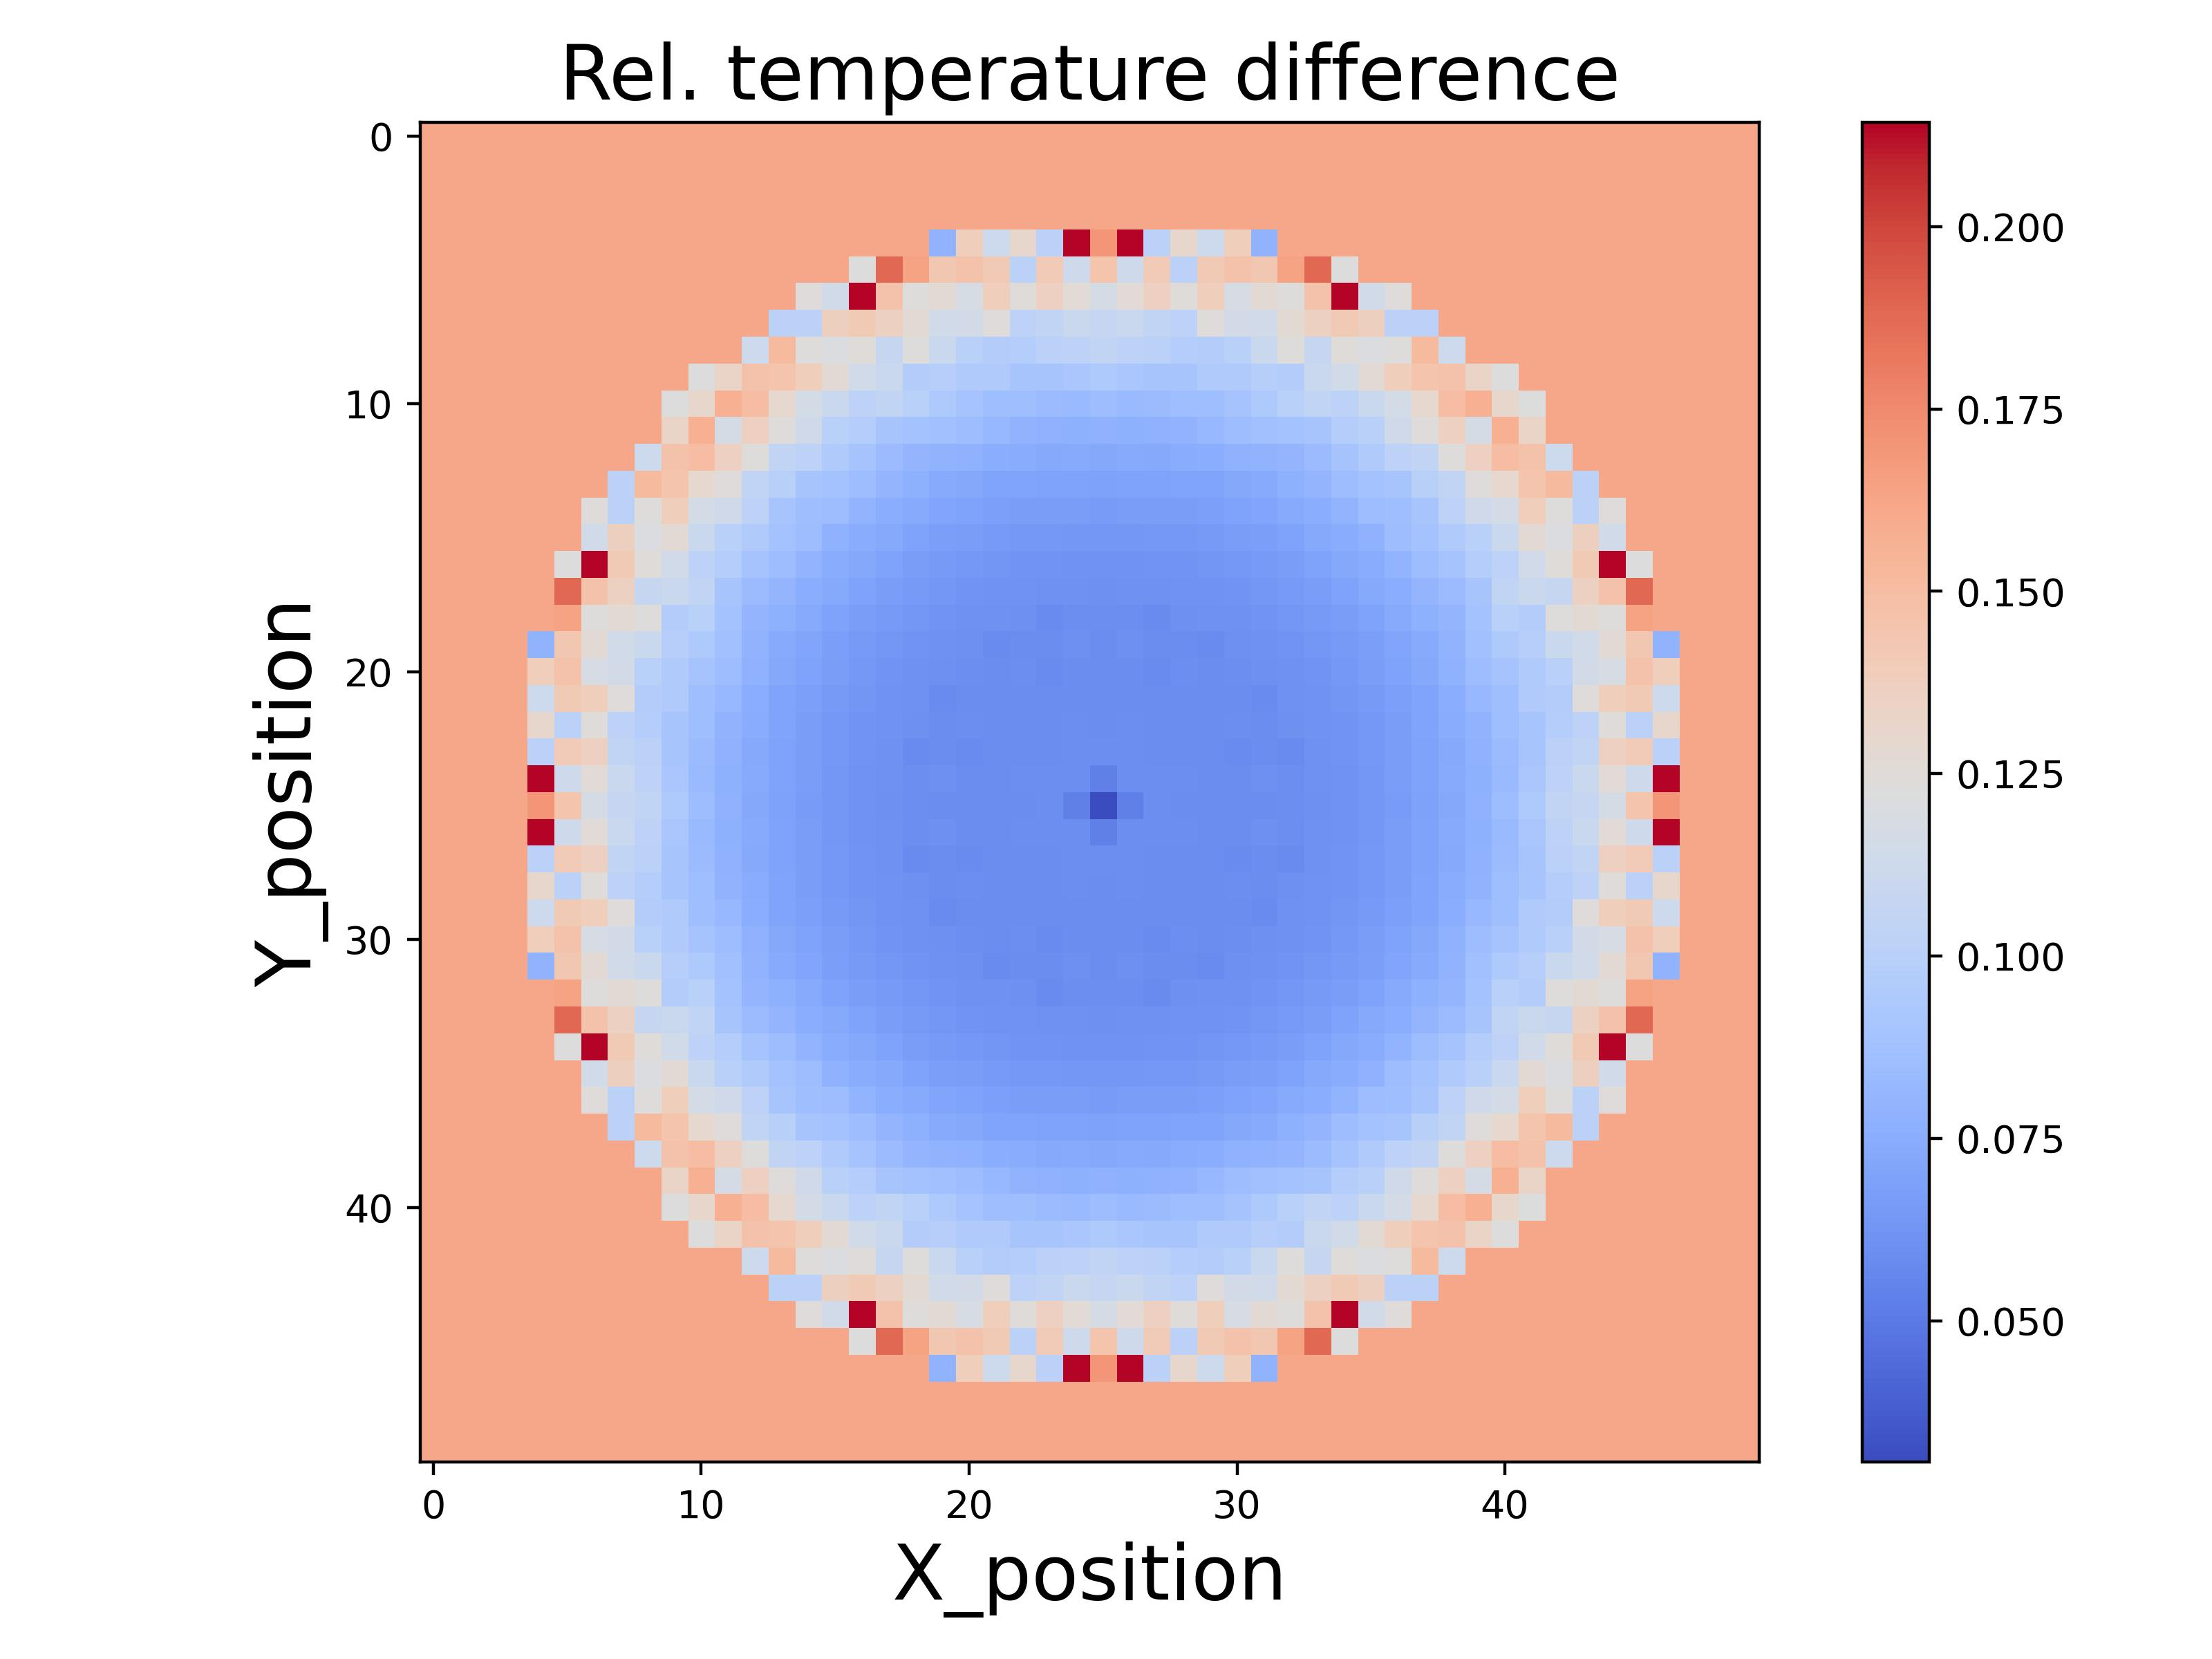
\includegraphics[width=\textwidth]{figures/raw_data/21/exp/T_bias.jpg}
        \end{subfigure}
        \begin{subfigure}{0.325\textwidth}
            \centering
            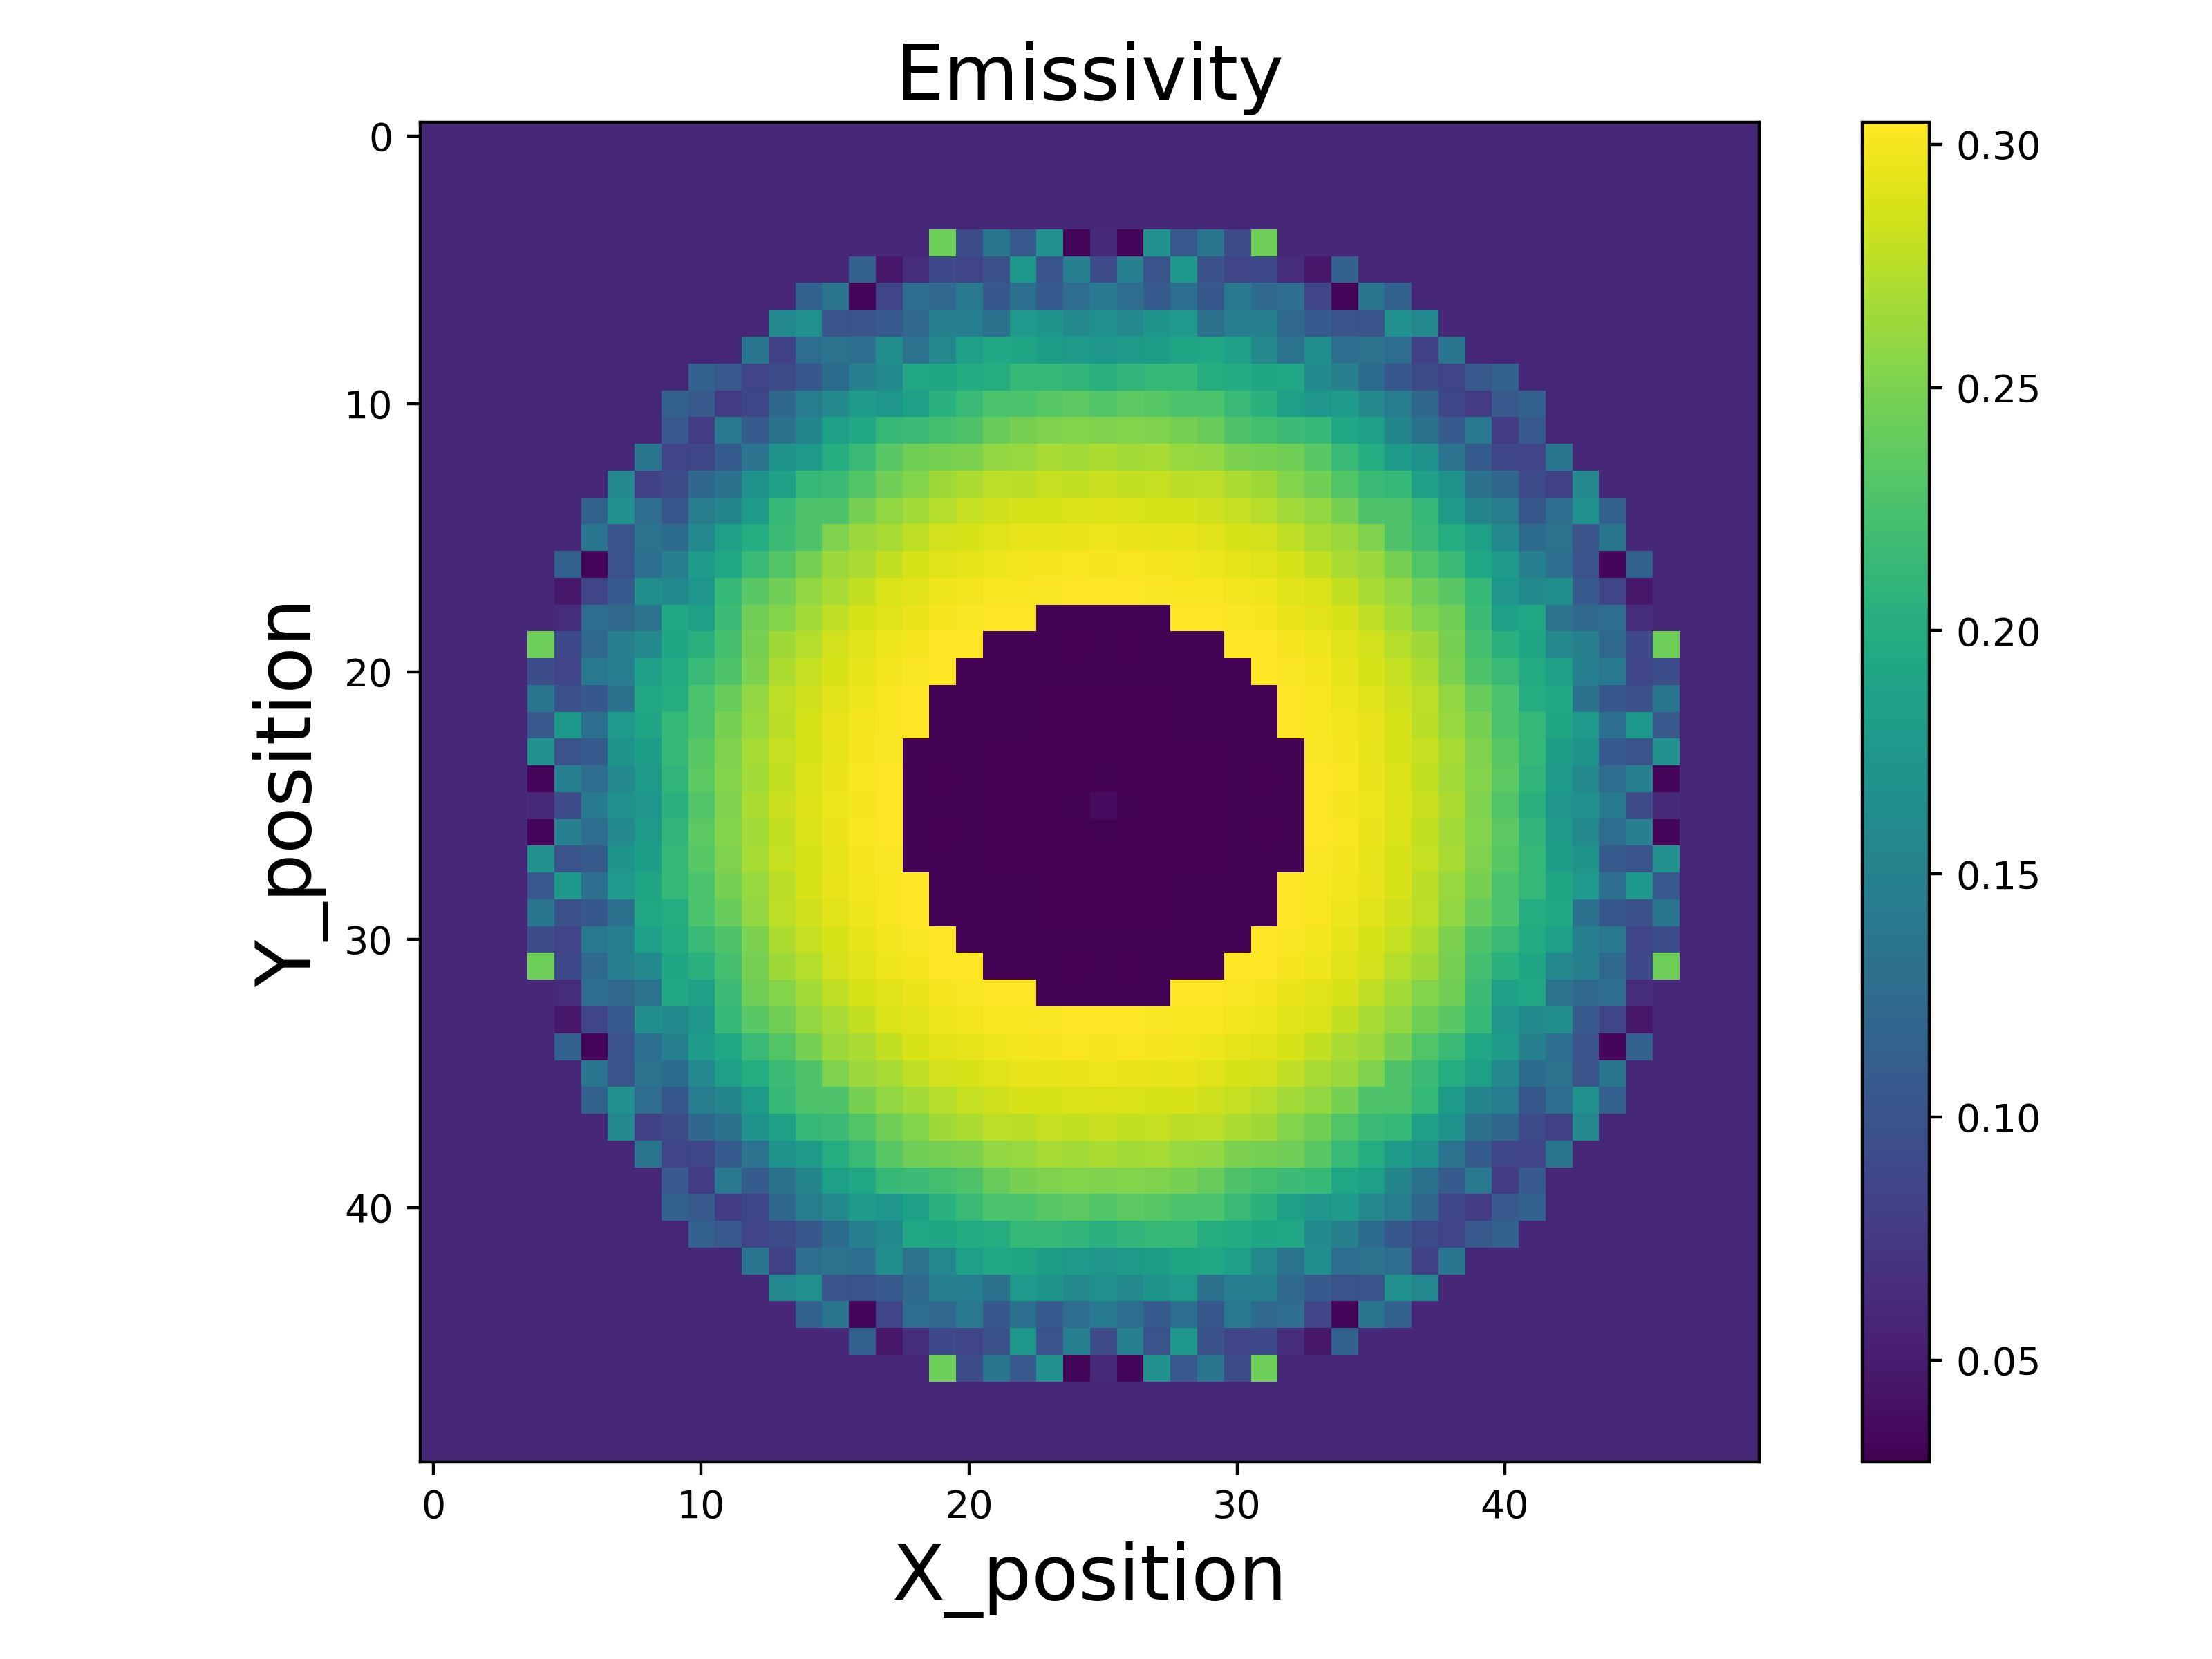
\includegraphics[width=\textwidth]{figures/raw_data/21/exp/emi_cal.jpg}
        \end{subfigure}
        \subcaption{Material based on model 1}
    \end{minipage}\\
    \begin{minipage}{\textwidth}
        \centering
        \begin{subfigure}{0.325\textwidth}
            \centering
            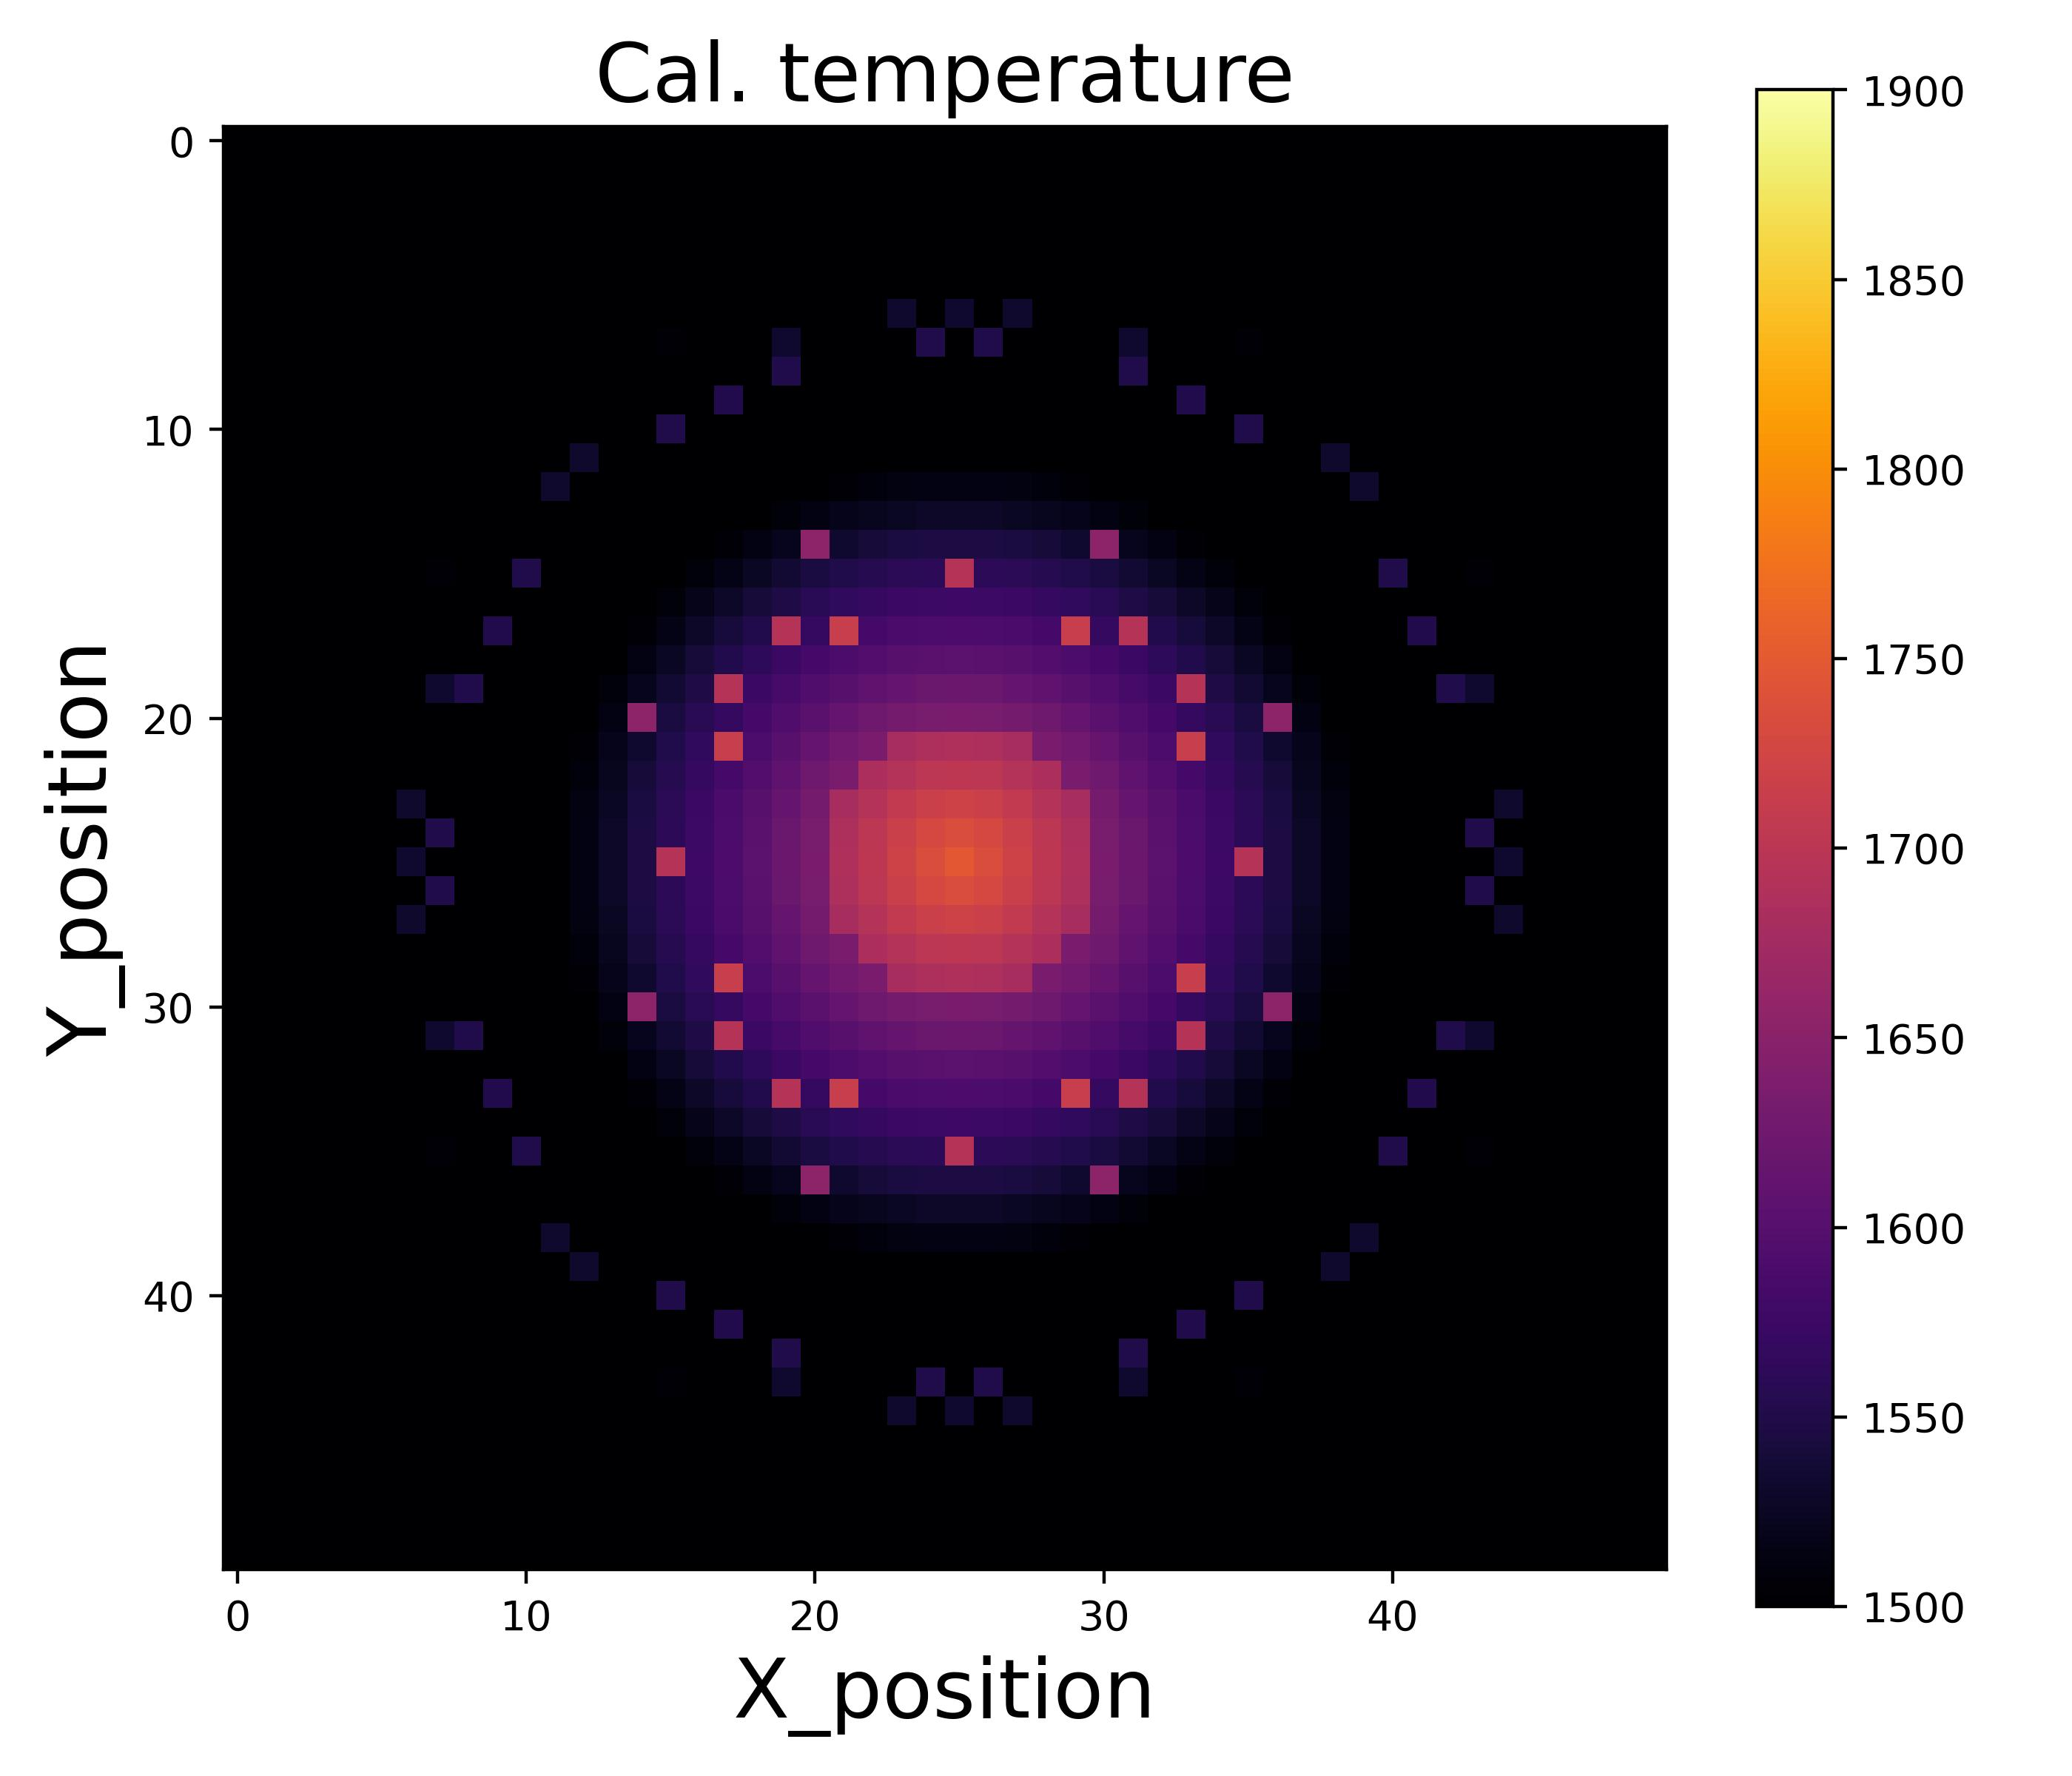
\includegraphics[width=\textwidth]{figures/raw_data/5/exp/T_cal.jpg}
        \end{subfigure}
        \begin{subfigure}{0.325\textwidth}
            \centering
            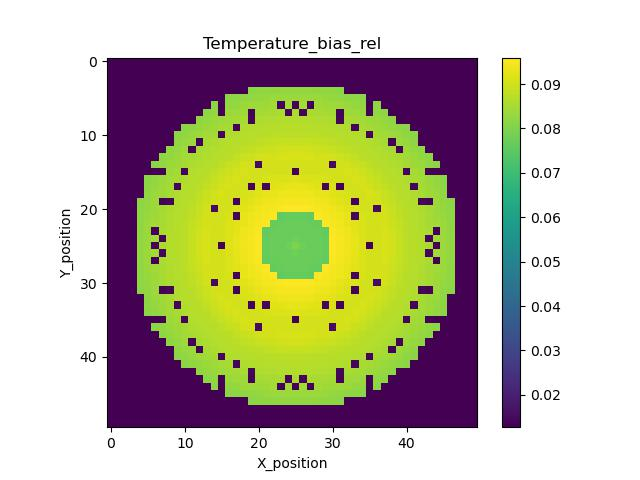
\includegraphics[width=\textwidth]{figures/raw_data/5/exp/T_bias.jpg}
        \end{subfigure}
        \begin{subfigure}{0.325\textwidth}
            \centering
            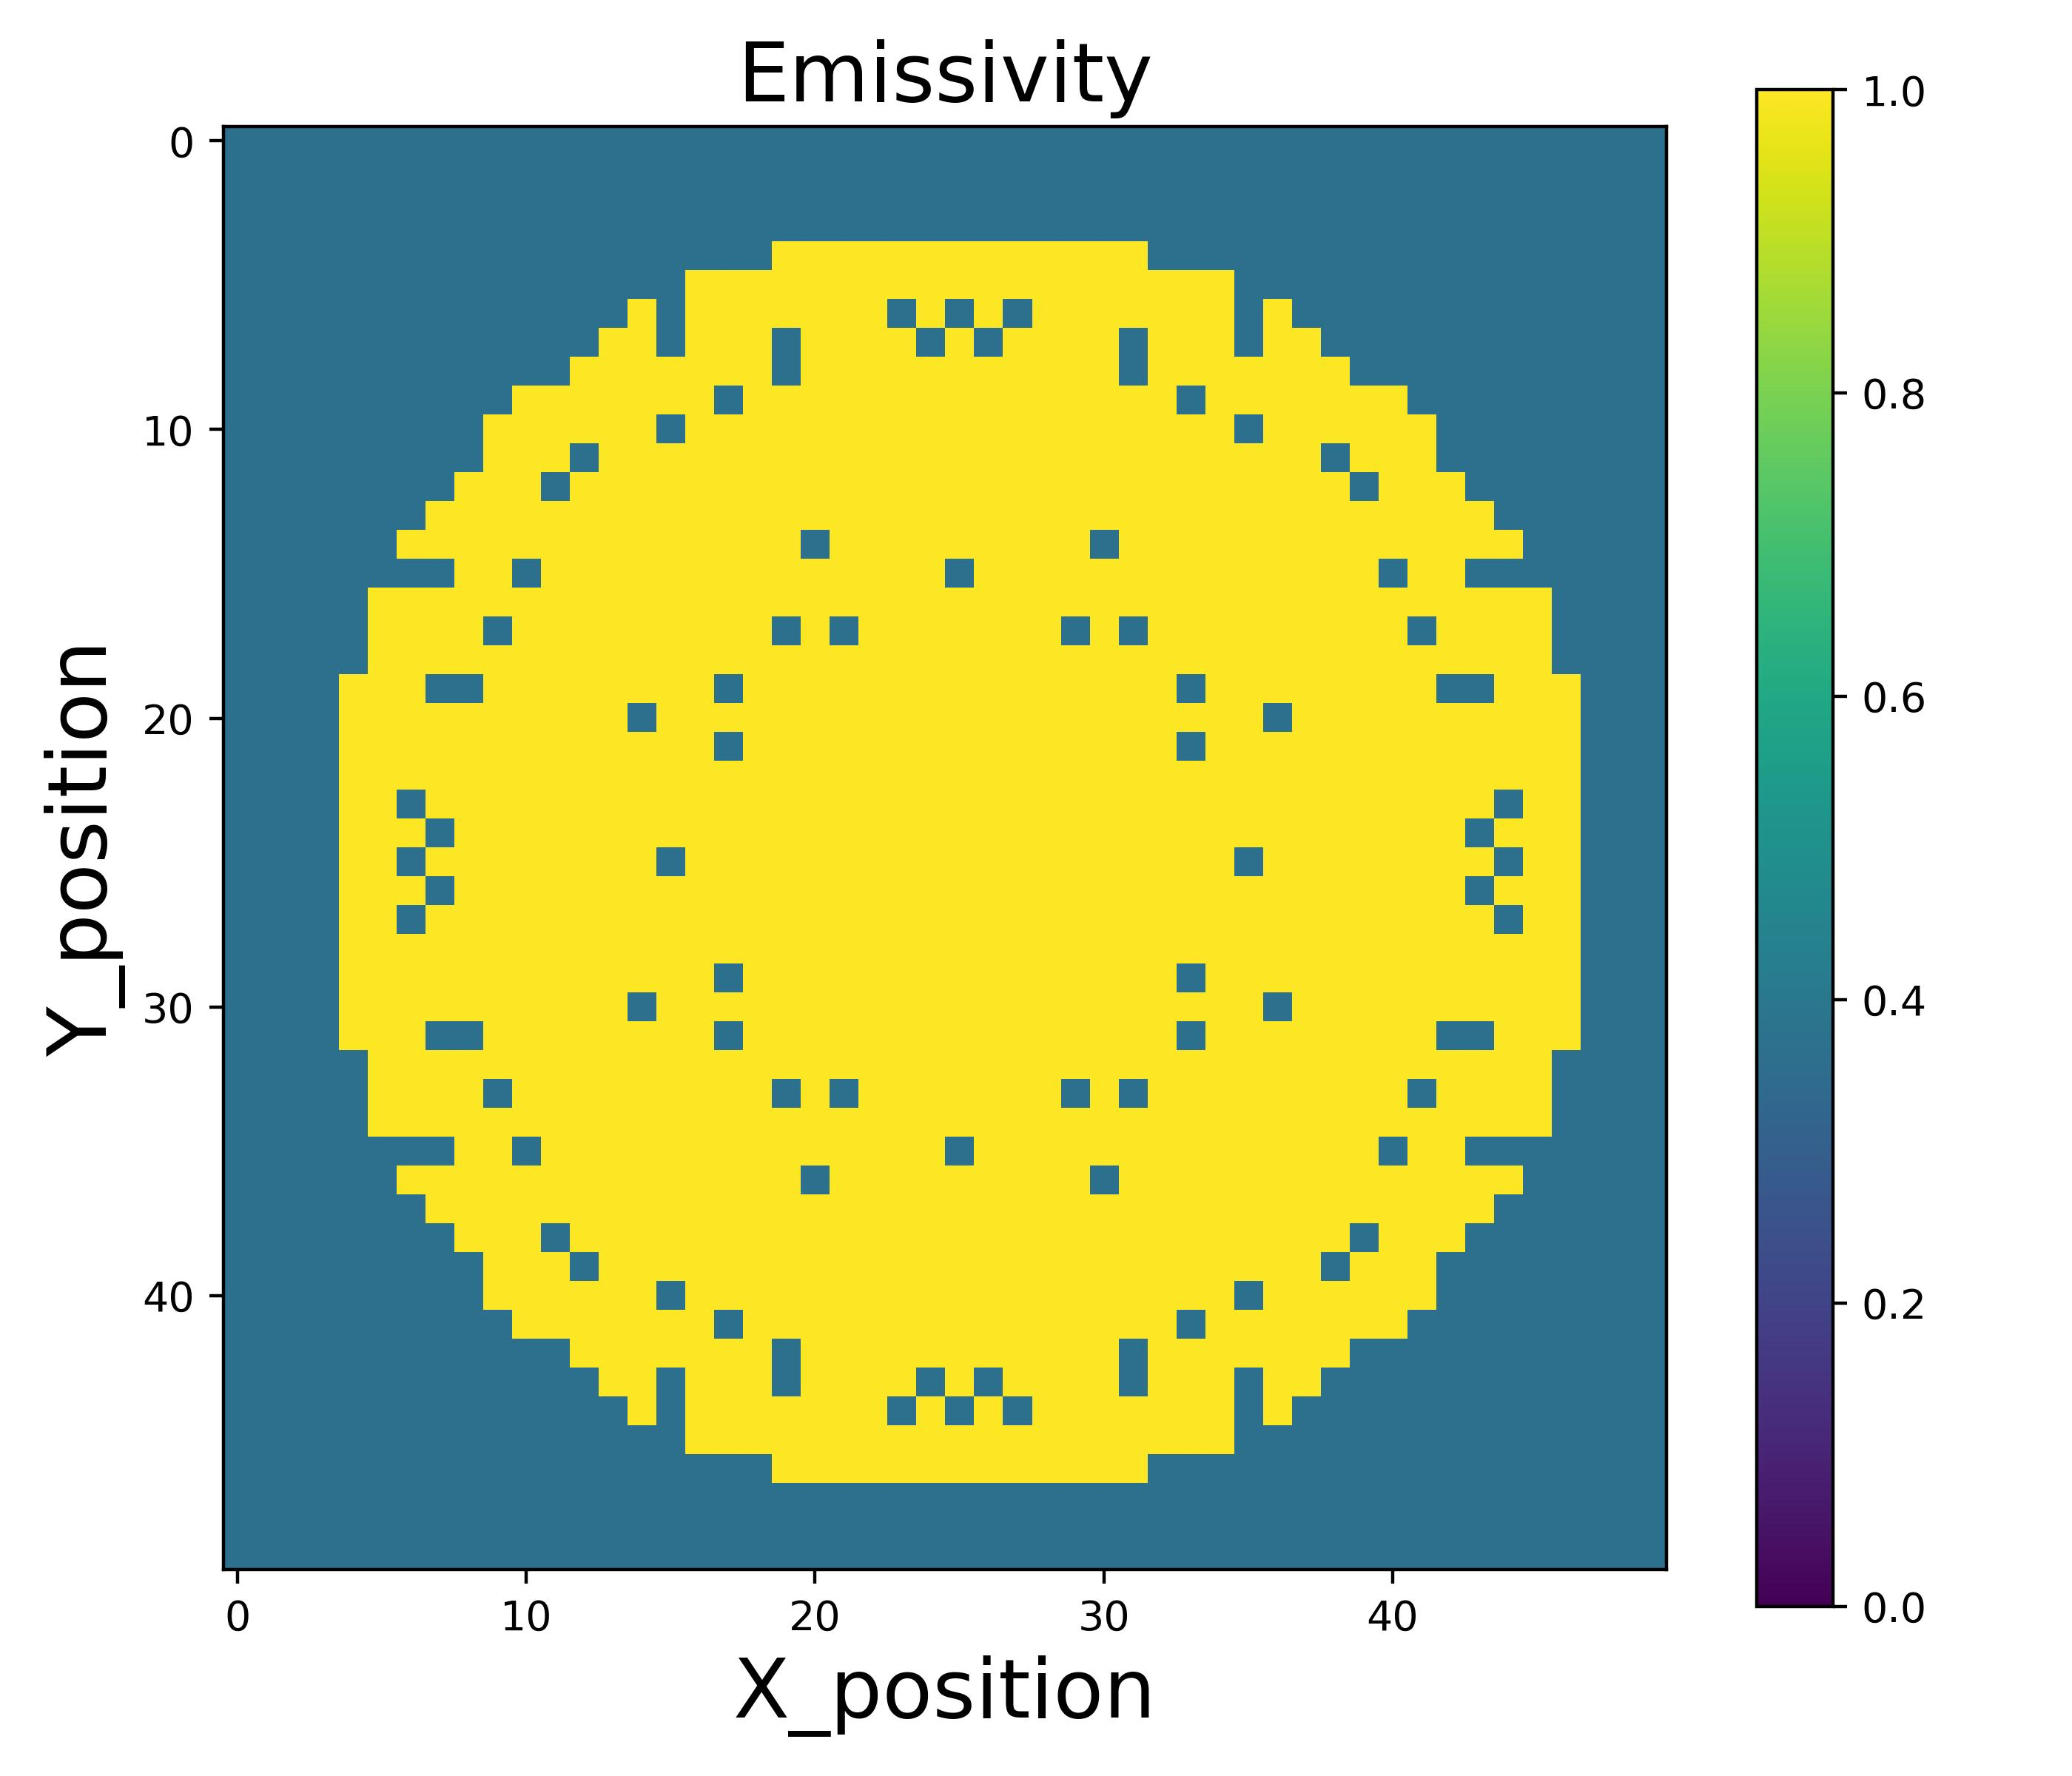
\includegraphics[width=\textwidth]{figures/raw_data/5/exp/emi_cal.jpg}
        \end{subfigure}
        \subcaption{Material based on real iron data}
    \end{minipage}
    \caption{Calculation results of exponential model}
    \label{fig: result_exponential_model}
\end{figure}


In the exponential model, the emissivity model follows the form of an 
exponential function. The two parameters in the emissivity model allow for 
translation and deformation of the exponential function. This enables the 
temperature estimation algorithm to be applicable to a wider range of materials 
with different emissivity characteristics. Fig.\ref{fig: result_exponential_model} 
presents the results of this temperature estimation algorithm for materials 
based on \mbox{model 1} and real iron.


Due to the physical meaning of emissivity, the value of emissivity is defined 
within the range of 0 to 1. Thus, constraints must be imposed on the 
emissivity model. Thus, calculated from Eq.\ref{eq: emi_exp}, the following 
constraints can be introduced:


\begin{equation}
    -a \cdot \lambda_{norm} - b \leq 0
\end{equation}


Therefore, the derivative of emissivity with respect to wavelength is obtained as:


\begin{equation}
    \frac{d\varepsilon(\lambda)}{d\lambda_{norm}} = -a \cdot e^{-a \cdot \lambda_{norm} - b}
\end{equation}

For each data point, the emissivity computed based on the exponential model 
is either monotonically increasing or decreasing, depending on the sign of 
parameter $a$. This characteristic of the model leads to an increase in 
computational speed and a decrease in 
computational accuracy when strong non-monotonic behavior is observed in 
the emissivity characteristics of the material.

In Fig.\ref{fig: result_exponential_model}, it is evident that material based on 
\mbox{model 1} exhibits an almost linear relationship between emissivity and 
wavelength in the liquid state. This enables the temperature estimation 
algorithm to accurately calculate the boundary region between the liquid and 
solid states and achieve high computational precision within the liquid 
state region.

However, when applying the temperature estimation algorithm to real iron data, 
it fails to accurately calculate the emissivity values. This discrepancy is due 
to the fluctuation observed in the emissivity of real iron as a function of 
wavelength. The emissivity of iron in the liquid state is closer to the 
numerically derived values of the algorithm than in the solid state, leading 
to erroneous conclusions of higher computational accuracy at the central points.


\subsubsection{Mixed model}
Eq.\ref{eq: emi_mix_gen} indicates that the mixed model is composed of two 
components: a low-temperature emissivity model and a high-temperature emissivity 
model. This approach offers a significant advantage as the temperature 
estimation algorithm can fit to the different emissivity 
characteristics observed in the liquid and solid regions. But the computational 
time has significantly increased due to the utilization of two different 
emissivity models.


\begin{equation}
    \label{eq: emi_mix}
    \varepsilon(\lambda) = \begin{cases} 
      a \cdot \lambda_{norm}^2 + b \cdot \lambda_{norm} + c &   T \leq T_{melt} \\
      \exp(-a \cdot \lambda_{norm} - b) & T > T_{melt}
    \end{cases}
  \end{equation}


In this work, the low-temperature emissivity model is represented by linear 
square model, while the high-temperature emissivity model is described using 
exponential model. This choice is driven by the fact that the emissivity of the 
hypothetical material exhibits significant fluctuations in the solid-state 
region, making it more suitable to be computed using linear 
square model to better capture its behavior. Conversely, in the liquid state 
region, the emissivity of the hypothetical material exhibits relatively smaller 
fluctuations, making it possible to use a faster computational 
exponential model without decreasing the accuracy.


\begin{figure}[htbp]
    \centering
    \begin{minipage}{\textwidth}
        \centering
        \begin{subfigure}{0.325\textwidth}
            \centering
            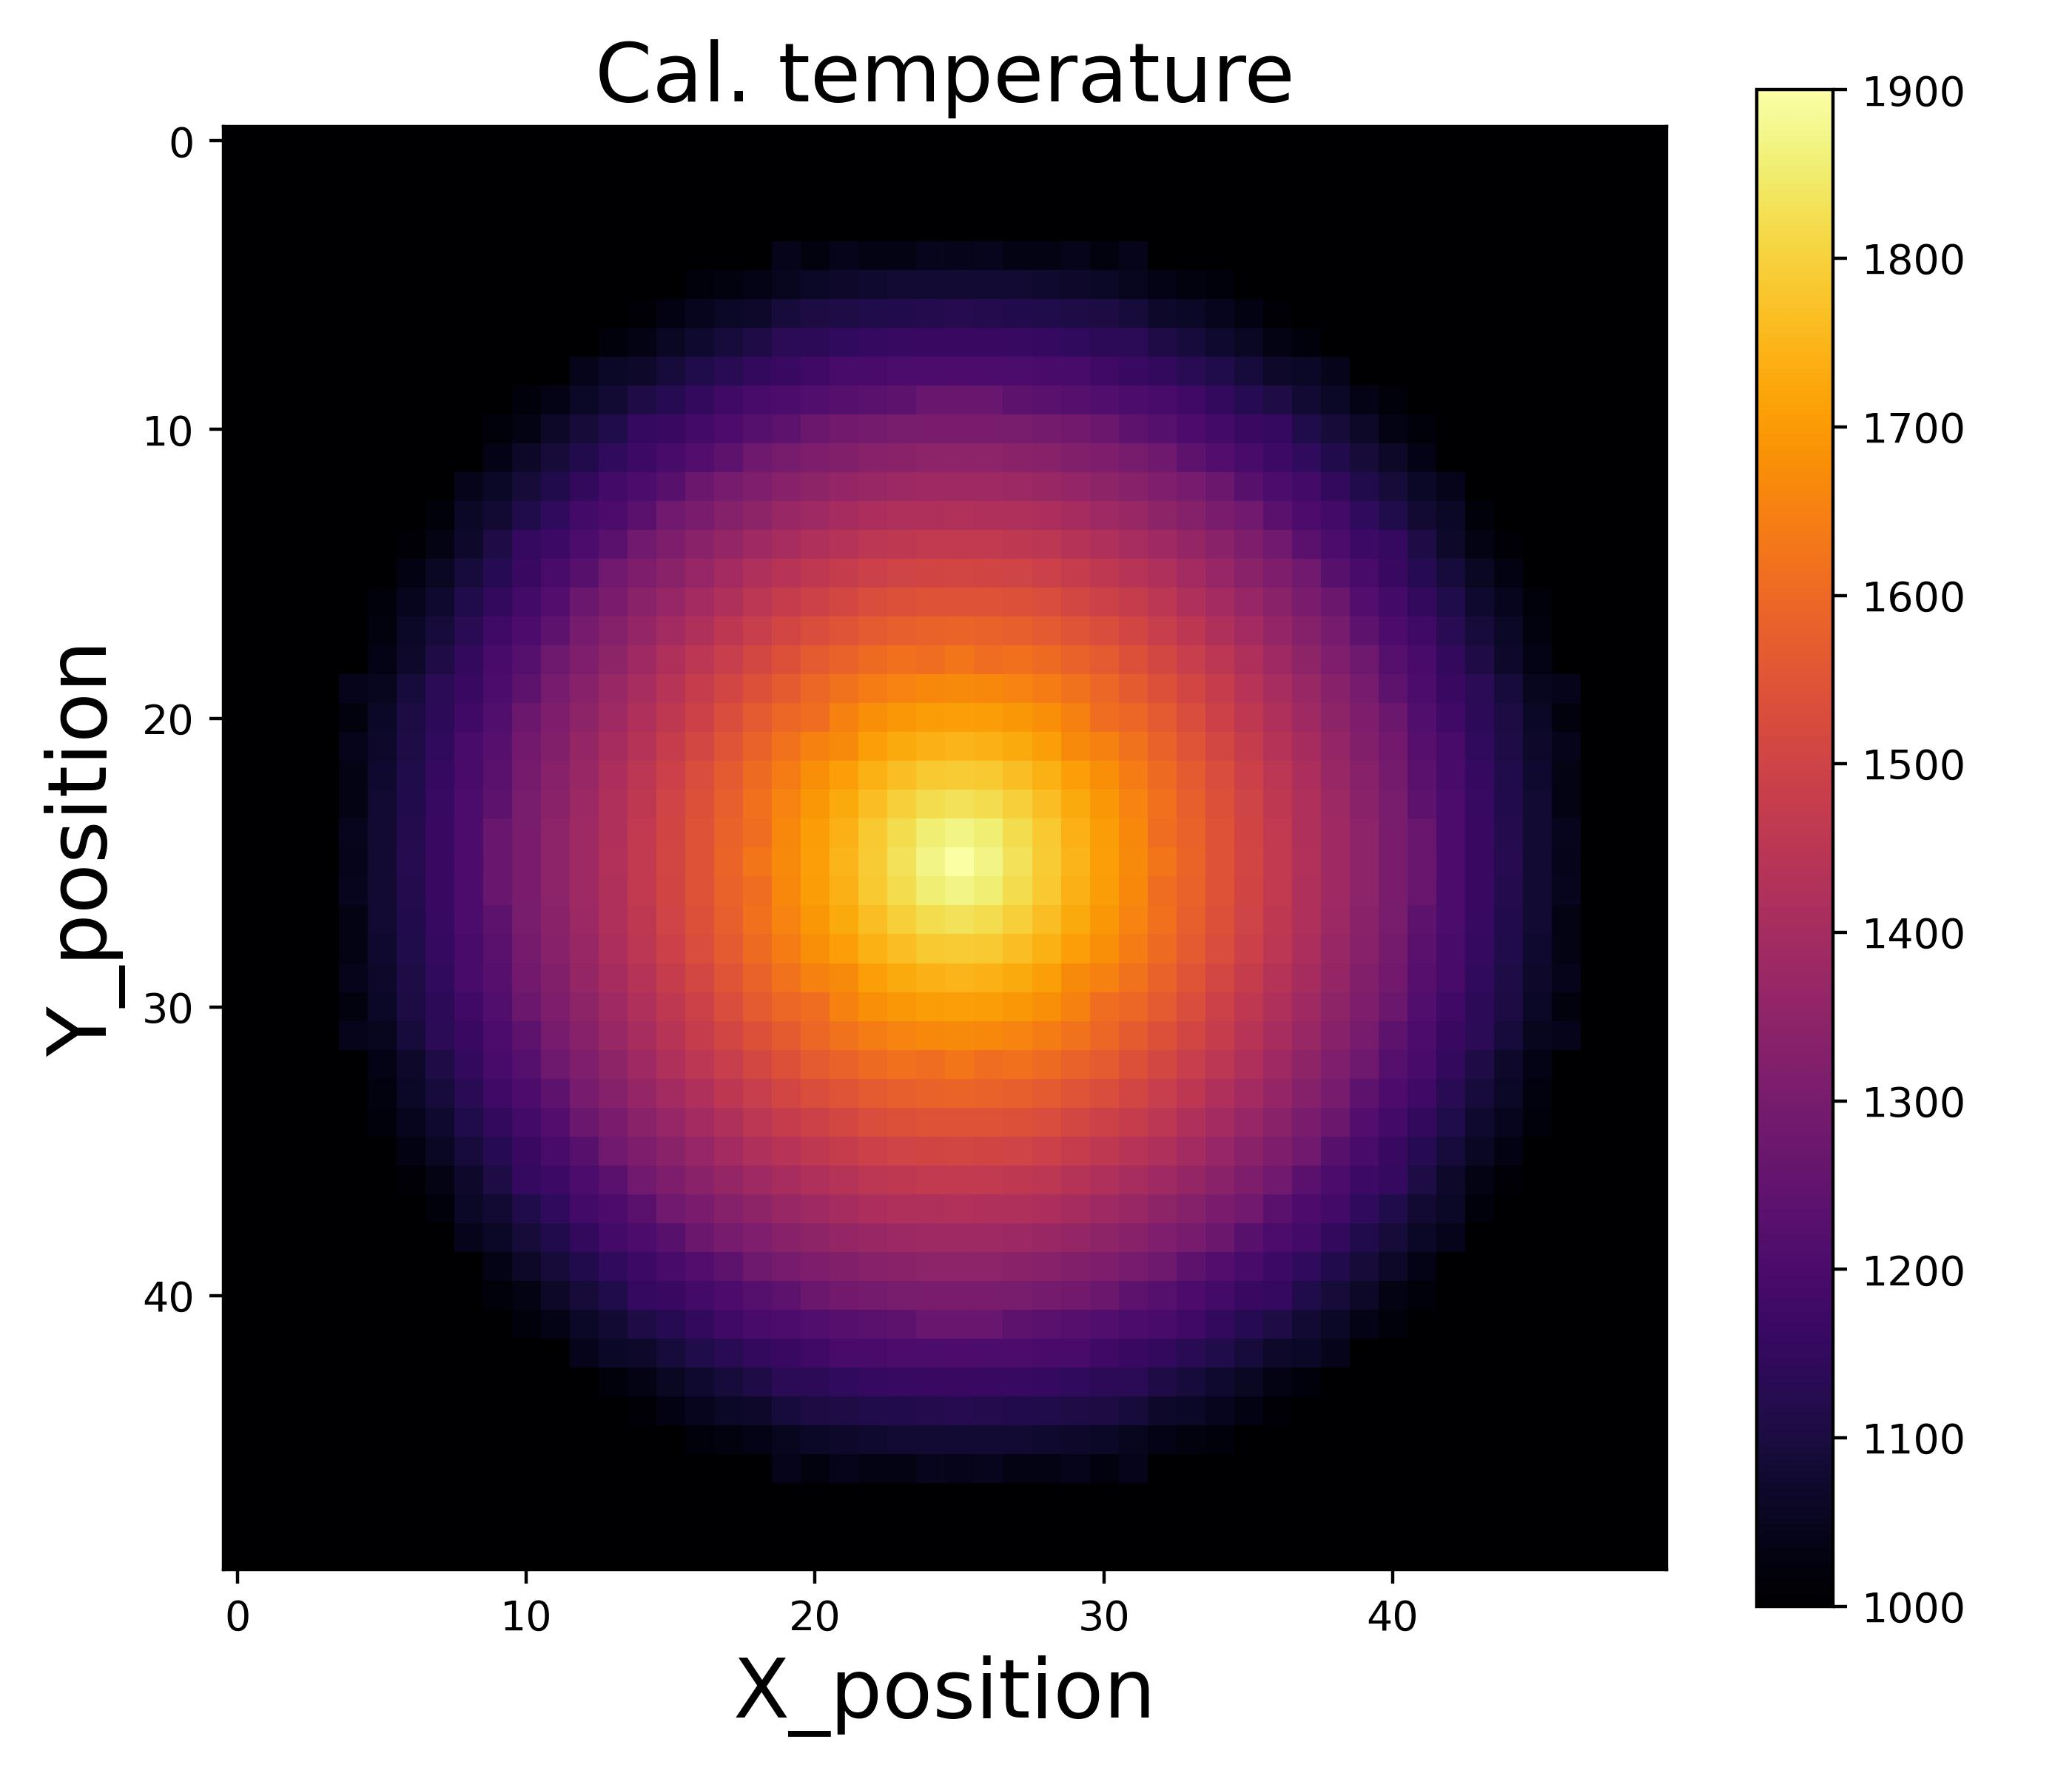
\includegraphics[width=\textwidth]{figures/raw_data/0/mix/T_cal.jpg}
        \end{subfigure}
        \begin{subfigure}{0.325\textwidth}
            \centering
            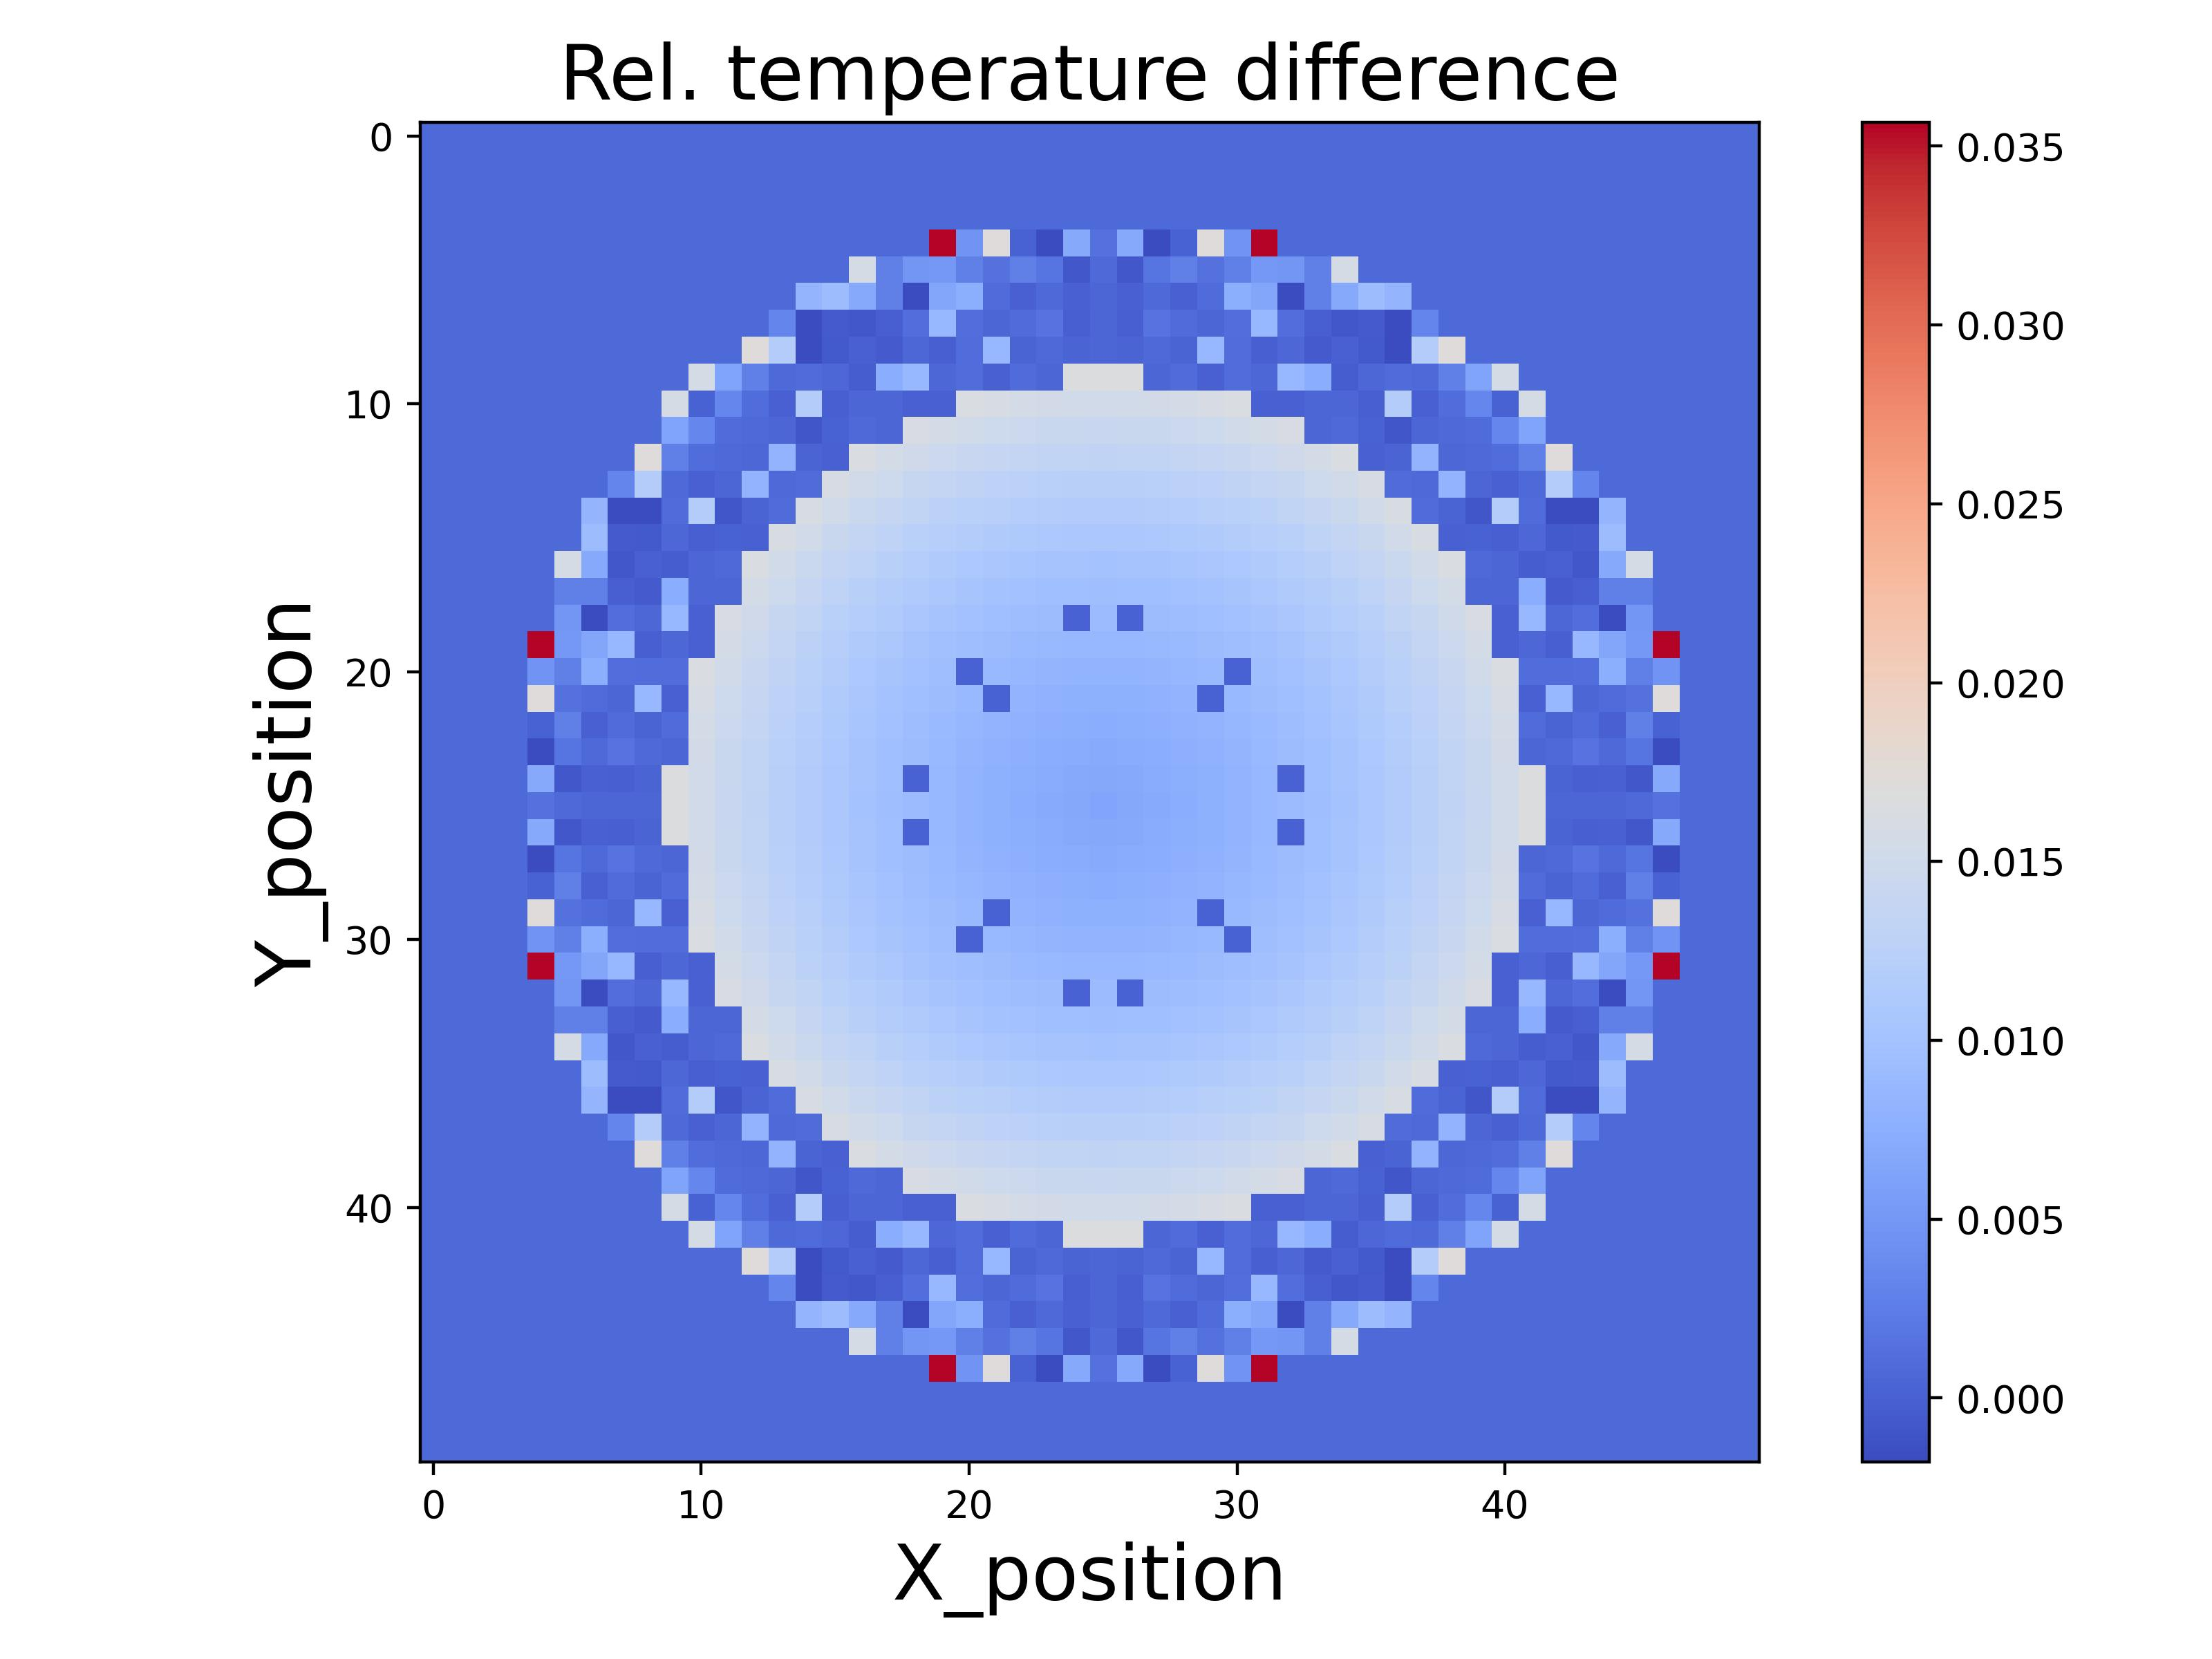
\includegraphics[width=\textwidth]{figures/raw_data/0/mix/T_bias.jpg}
        \end{subfigure}
        \begin{subfigure}{0.325\textwidth}
            \centering
            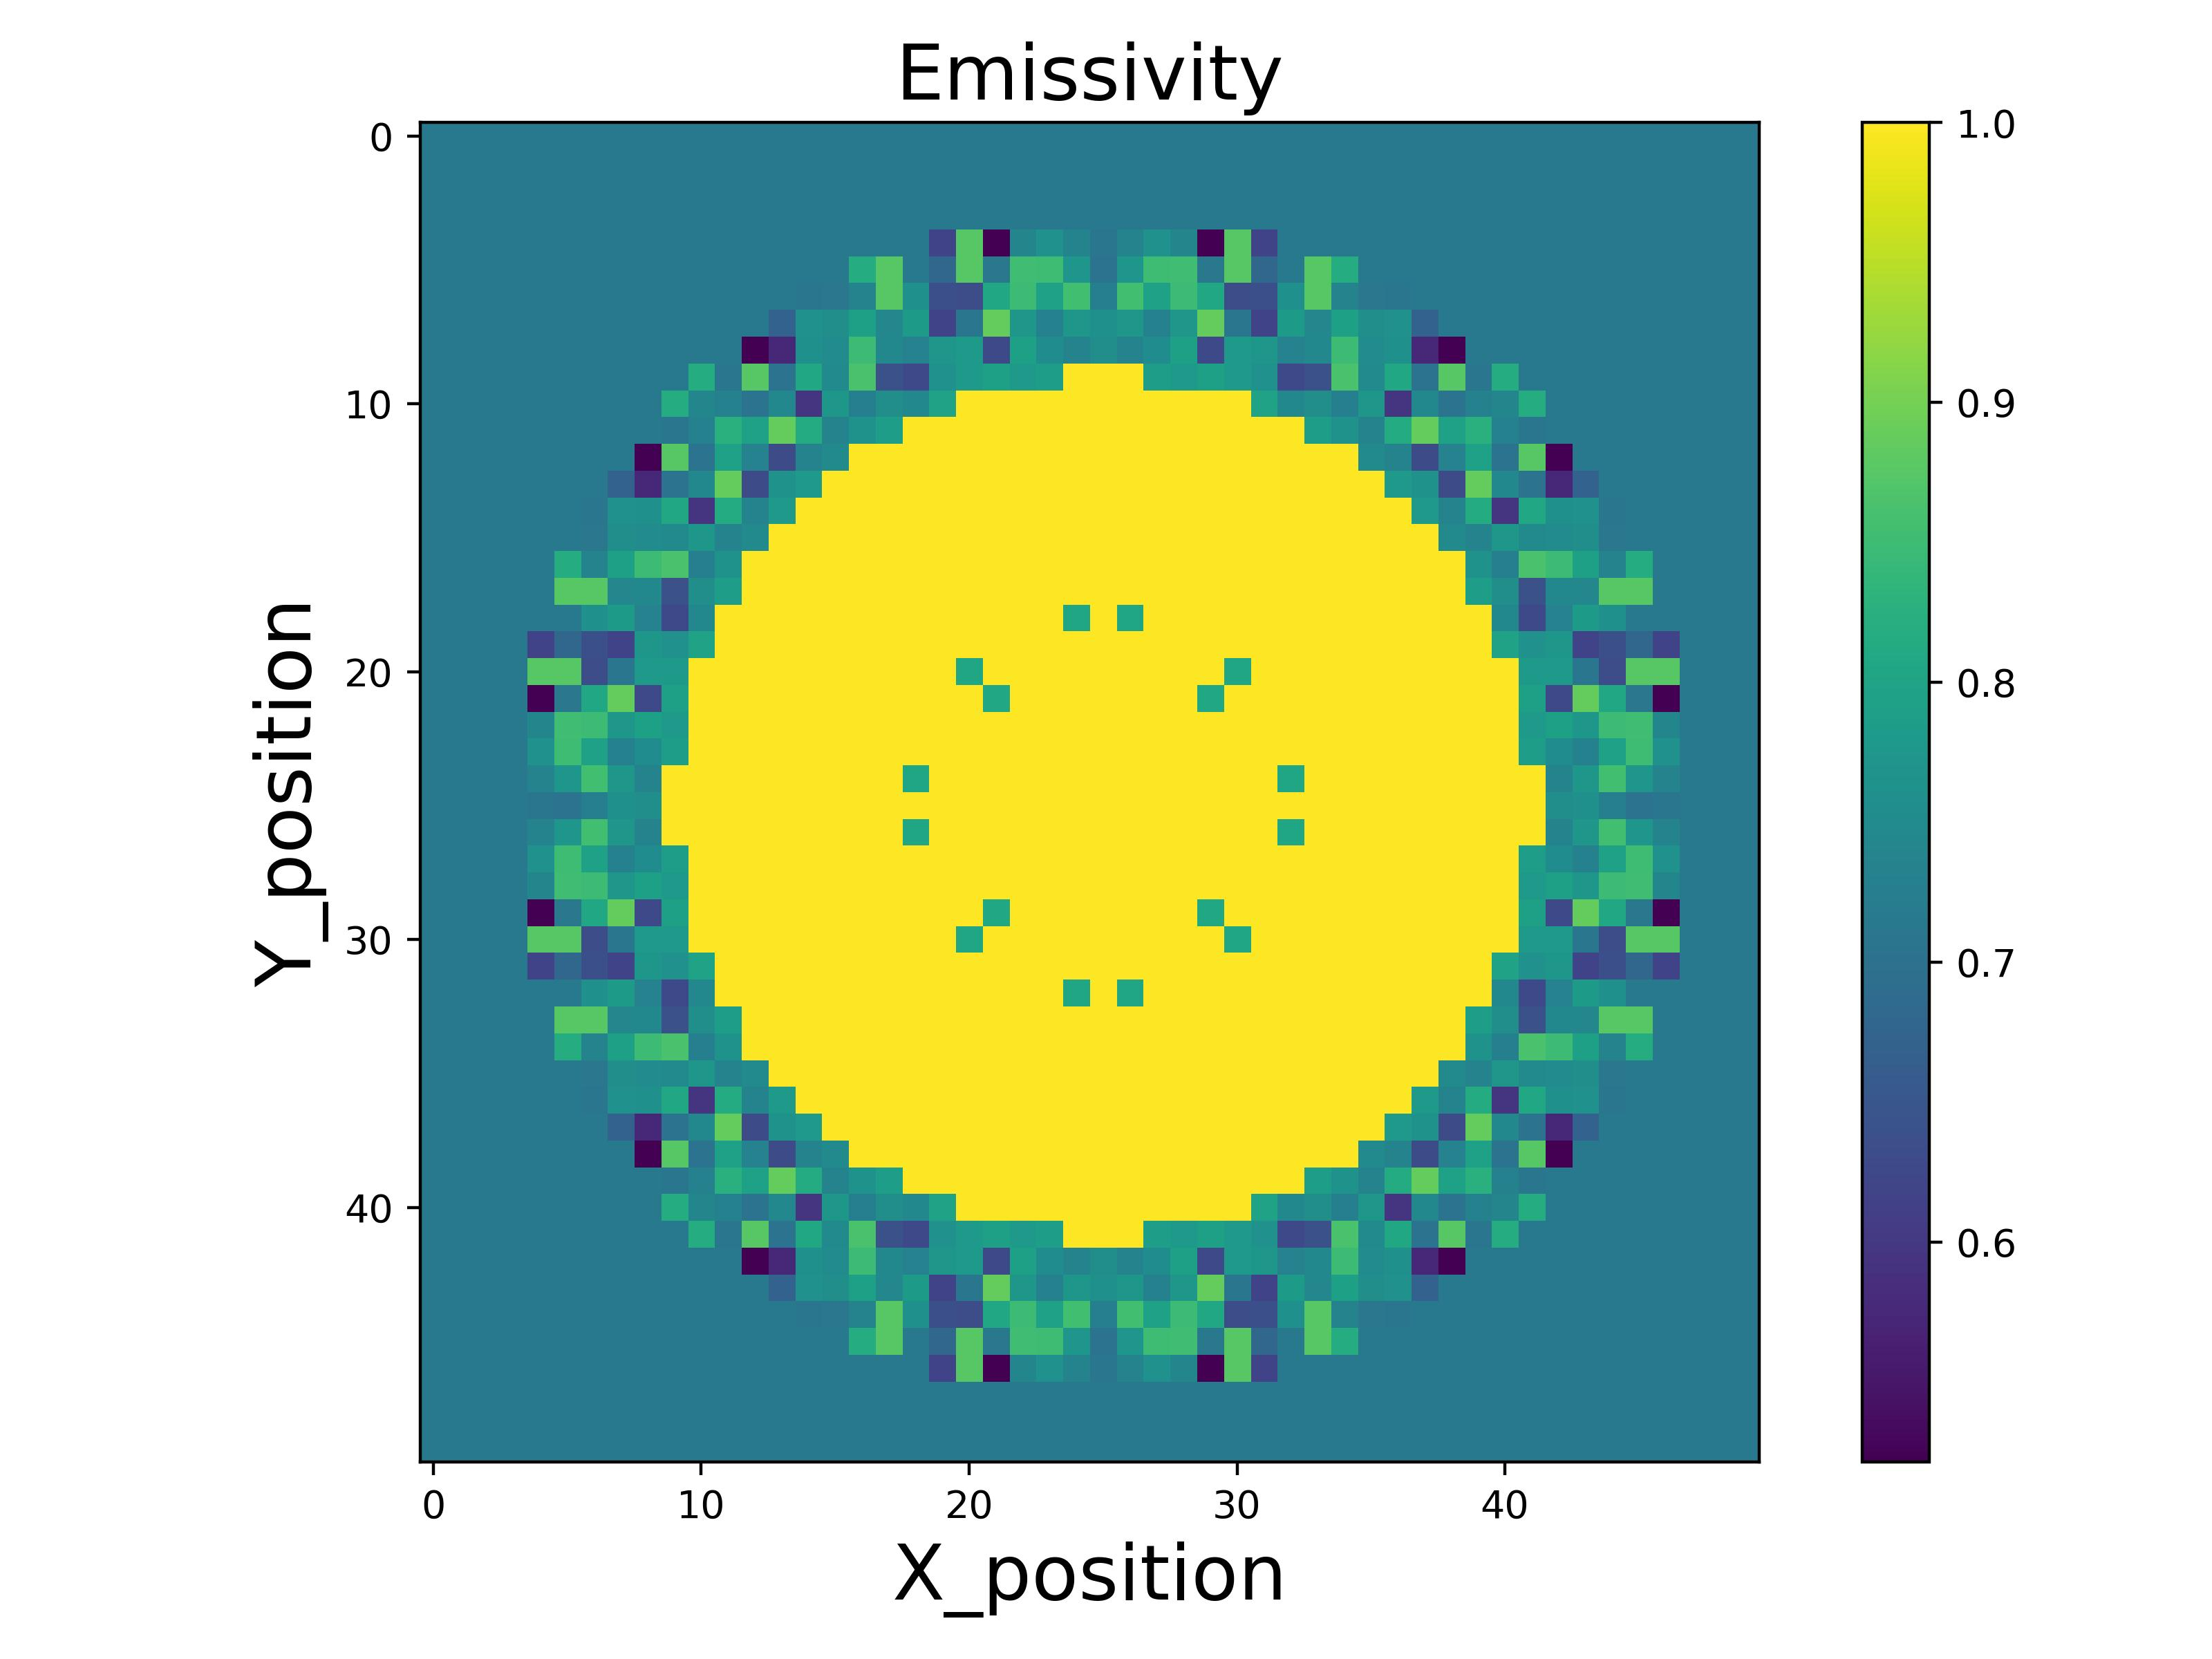
\includegraphics[width=\textwidth]{figures/raw_data/0/mix/emi_cal.jpg}
        \end{subfigure}
        \subcaption{Black body material}
    \end{minipage}\\
    \begin{minipage}{\textwidth}
        \centering
        \begin{subfigure}{0.325\textwidth}
            \centering
            \includegraphics[width=\textwidth]{figures/raw_data/21/mix/T_cal.jpg}
        \end{subfigure}
        \begin{subfigure}{0.325\textwidth}
            \centering
            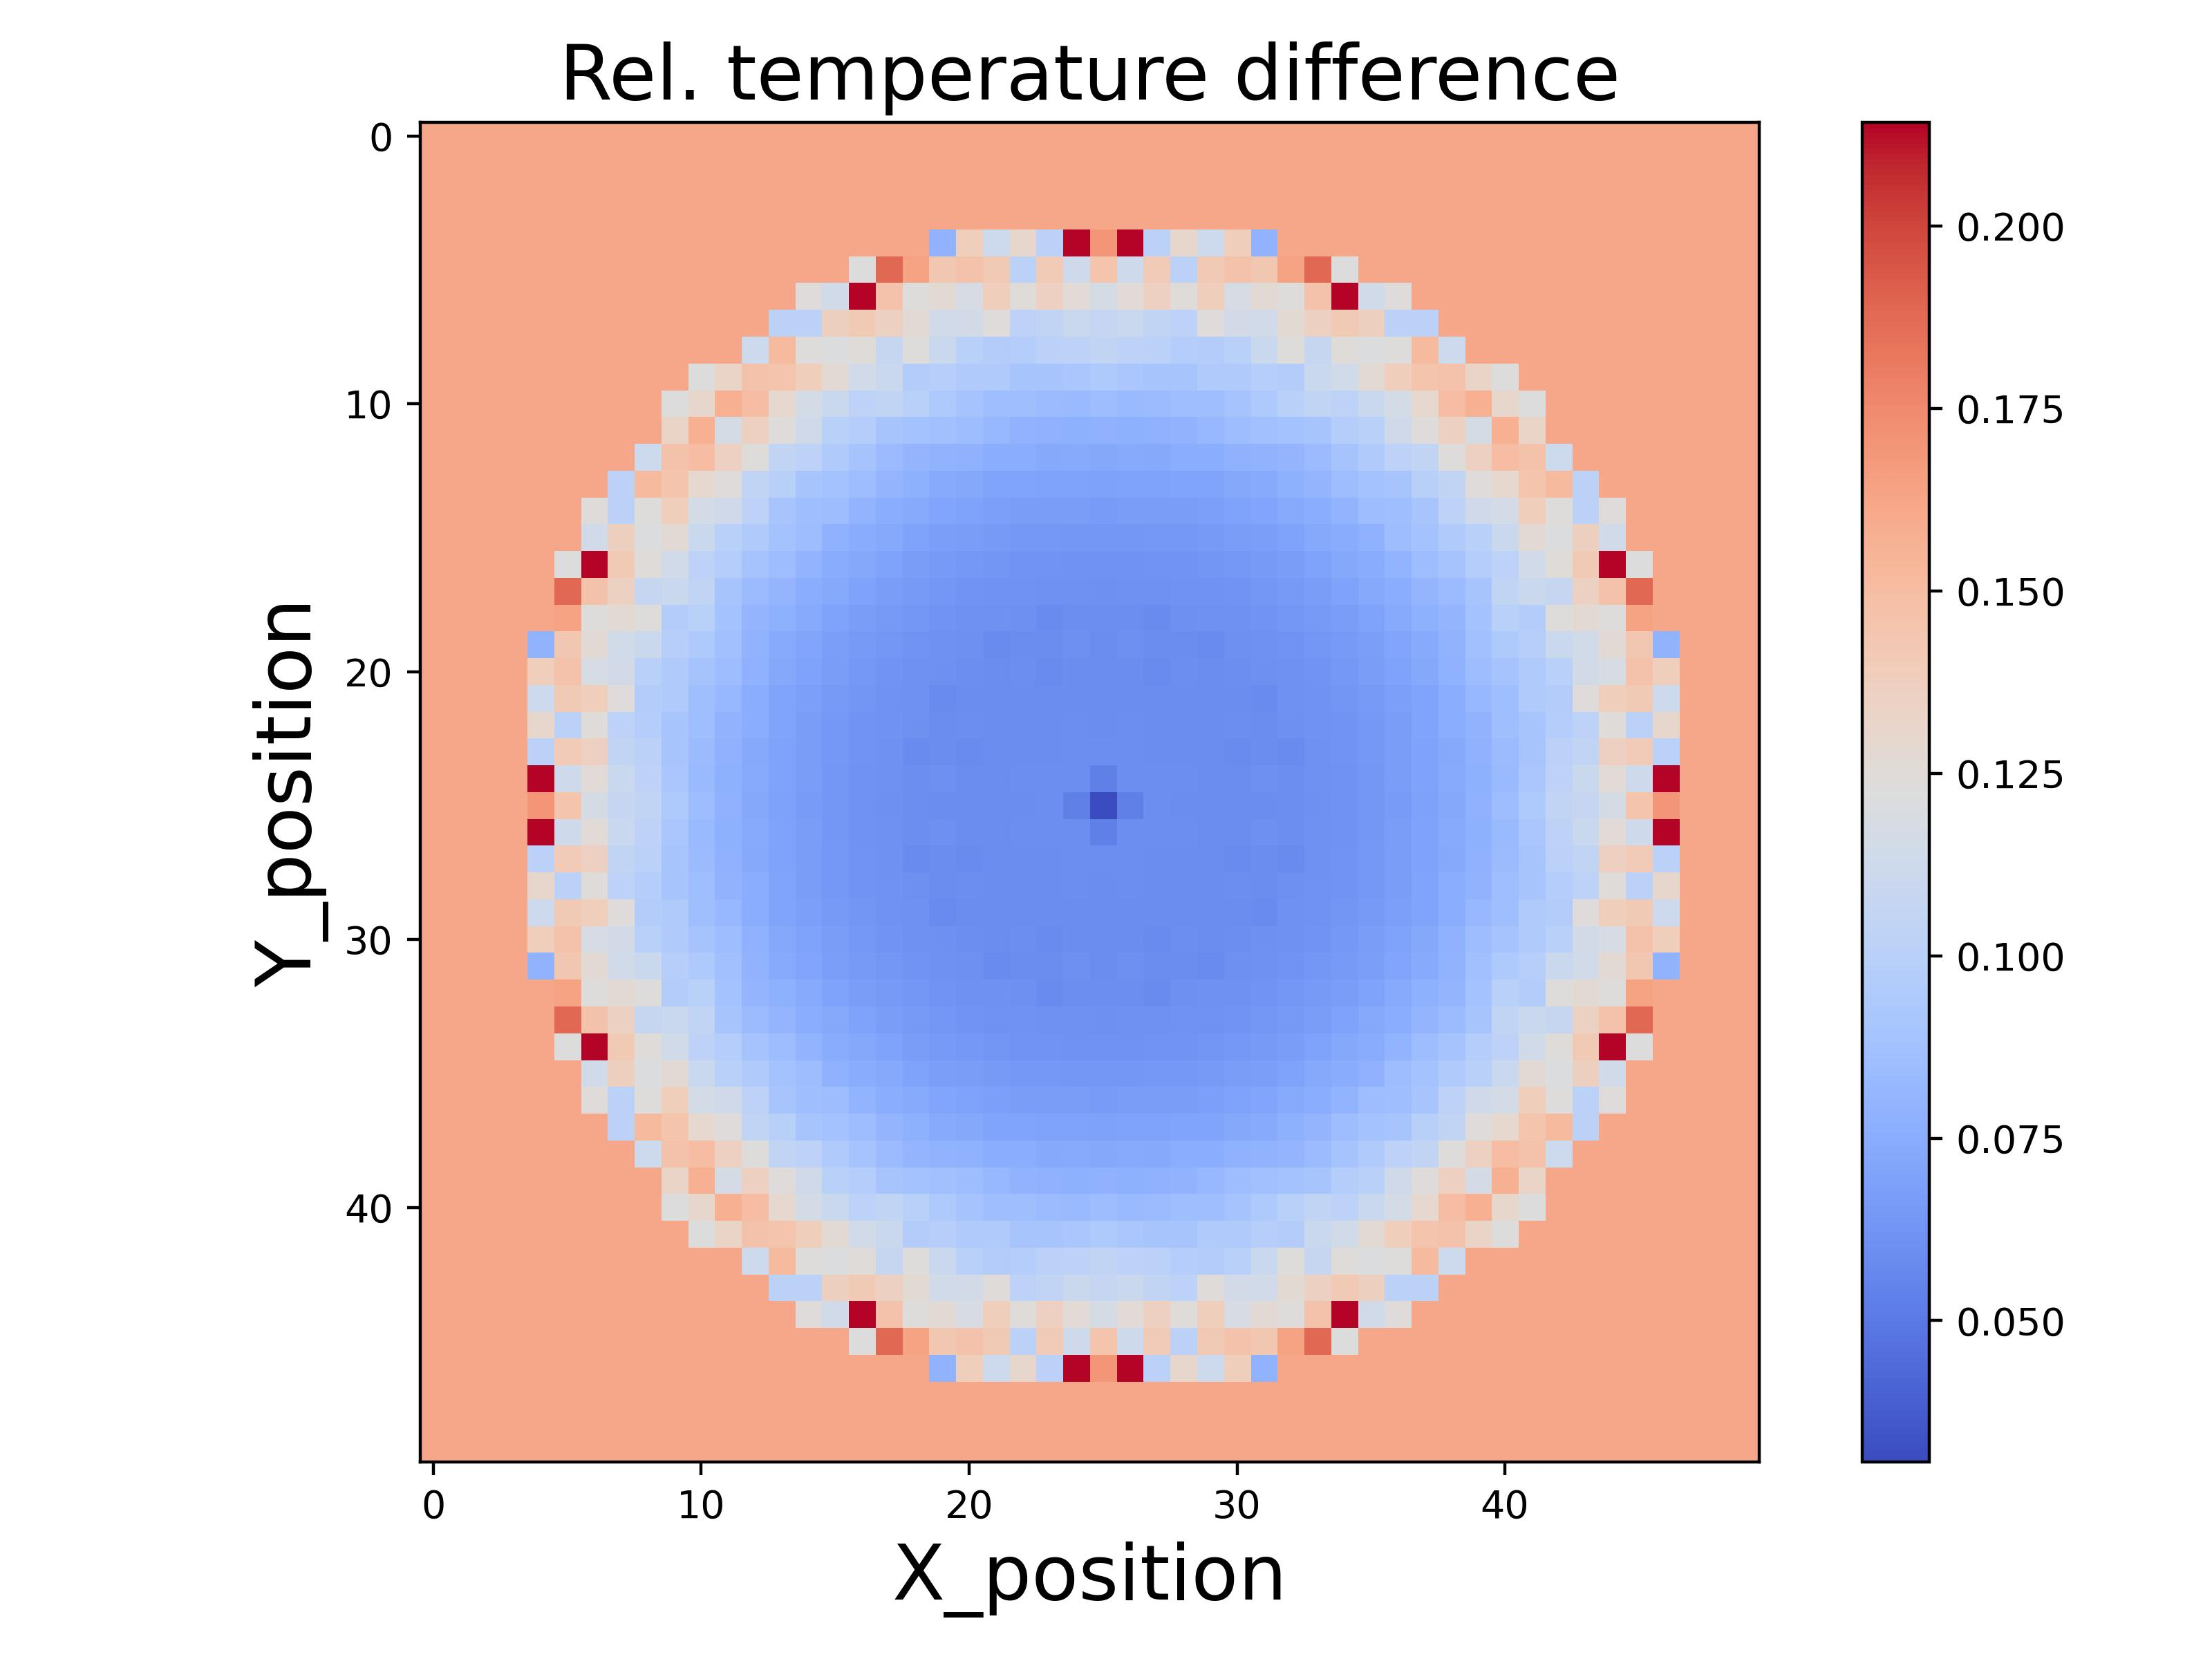
\includegraphics[width=\textwidth]{figures/raw_data/21/mix/T_bias.jpg}
        \end{subfigure}
        \begin{subfigure}{0.325\textwidth}
            \centering
            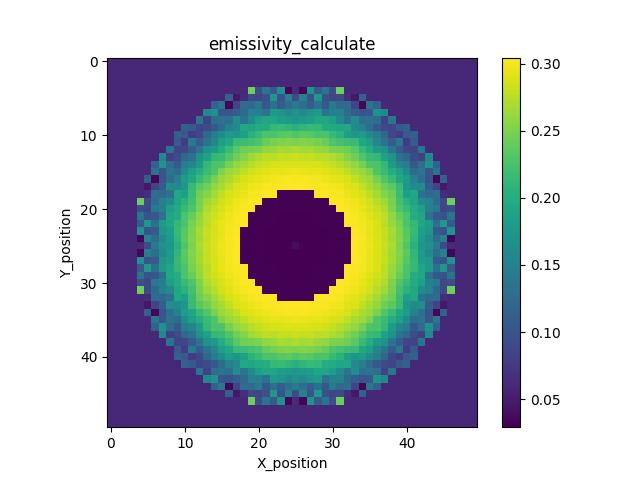
\includegraphics[width=\textwidth]{figures/raw_data/21/mix/emi_cal.jpg}
        \end{subfigure}
        \subcaption{Material based on model 1}
    \end{minipage}\\
    \begin{minipage}{\textwidth}
        \centering
        \begin{subfigure}{0.325\textwidth}
            \centering
            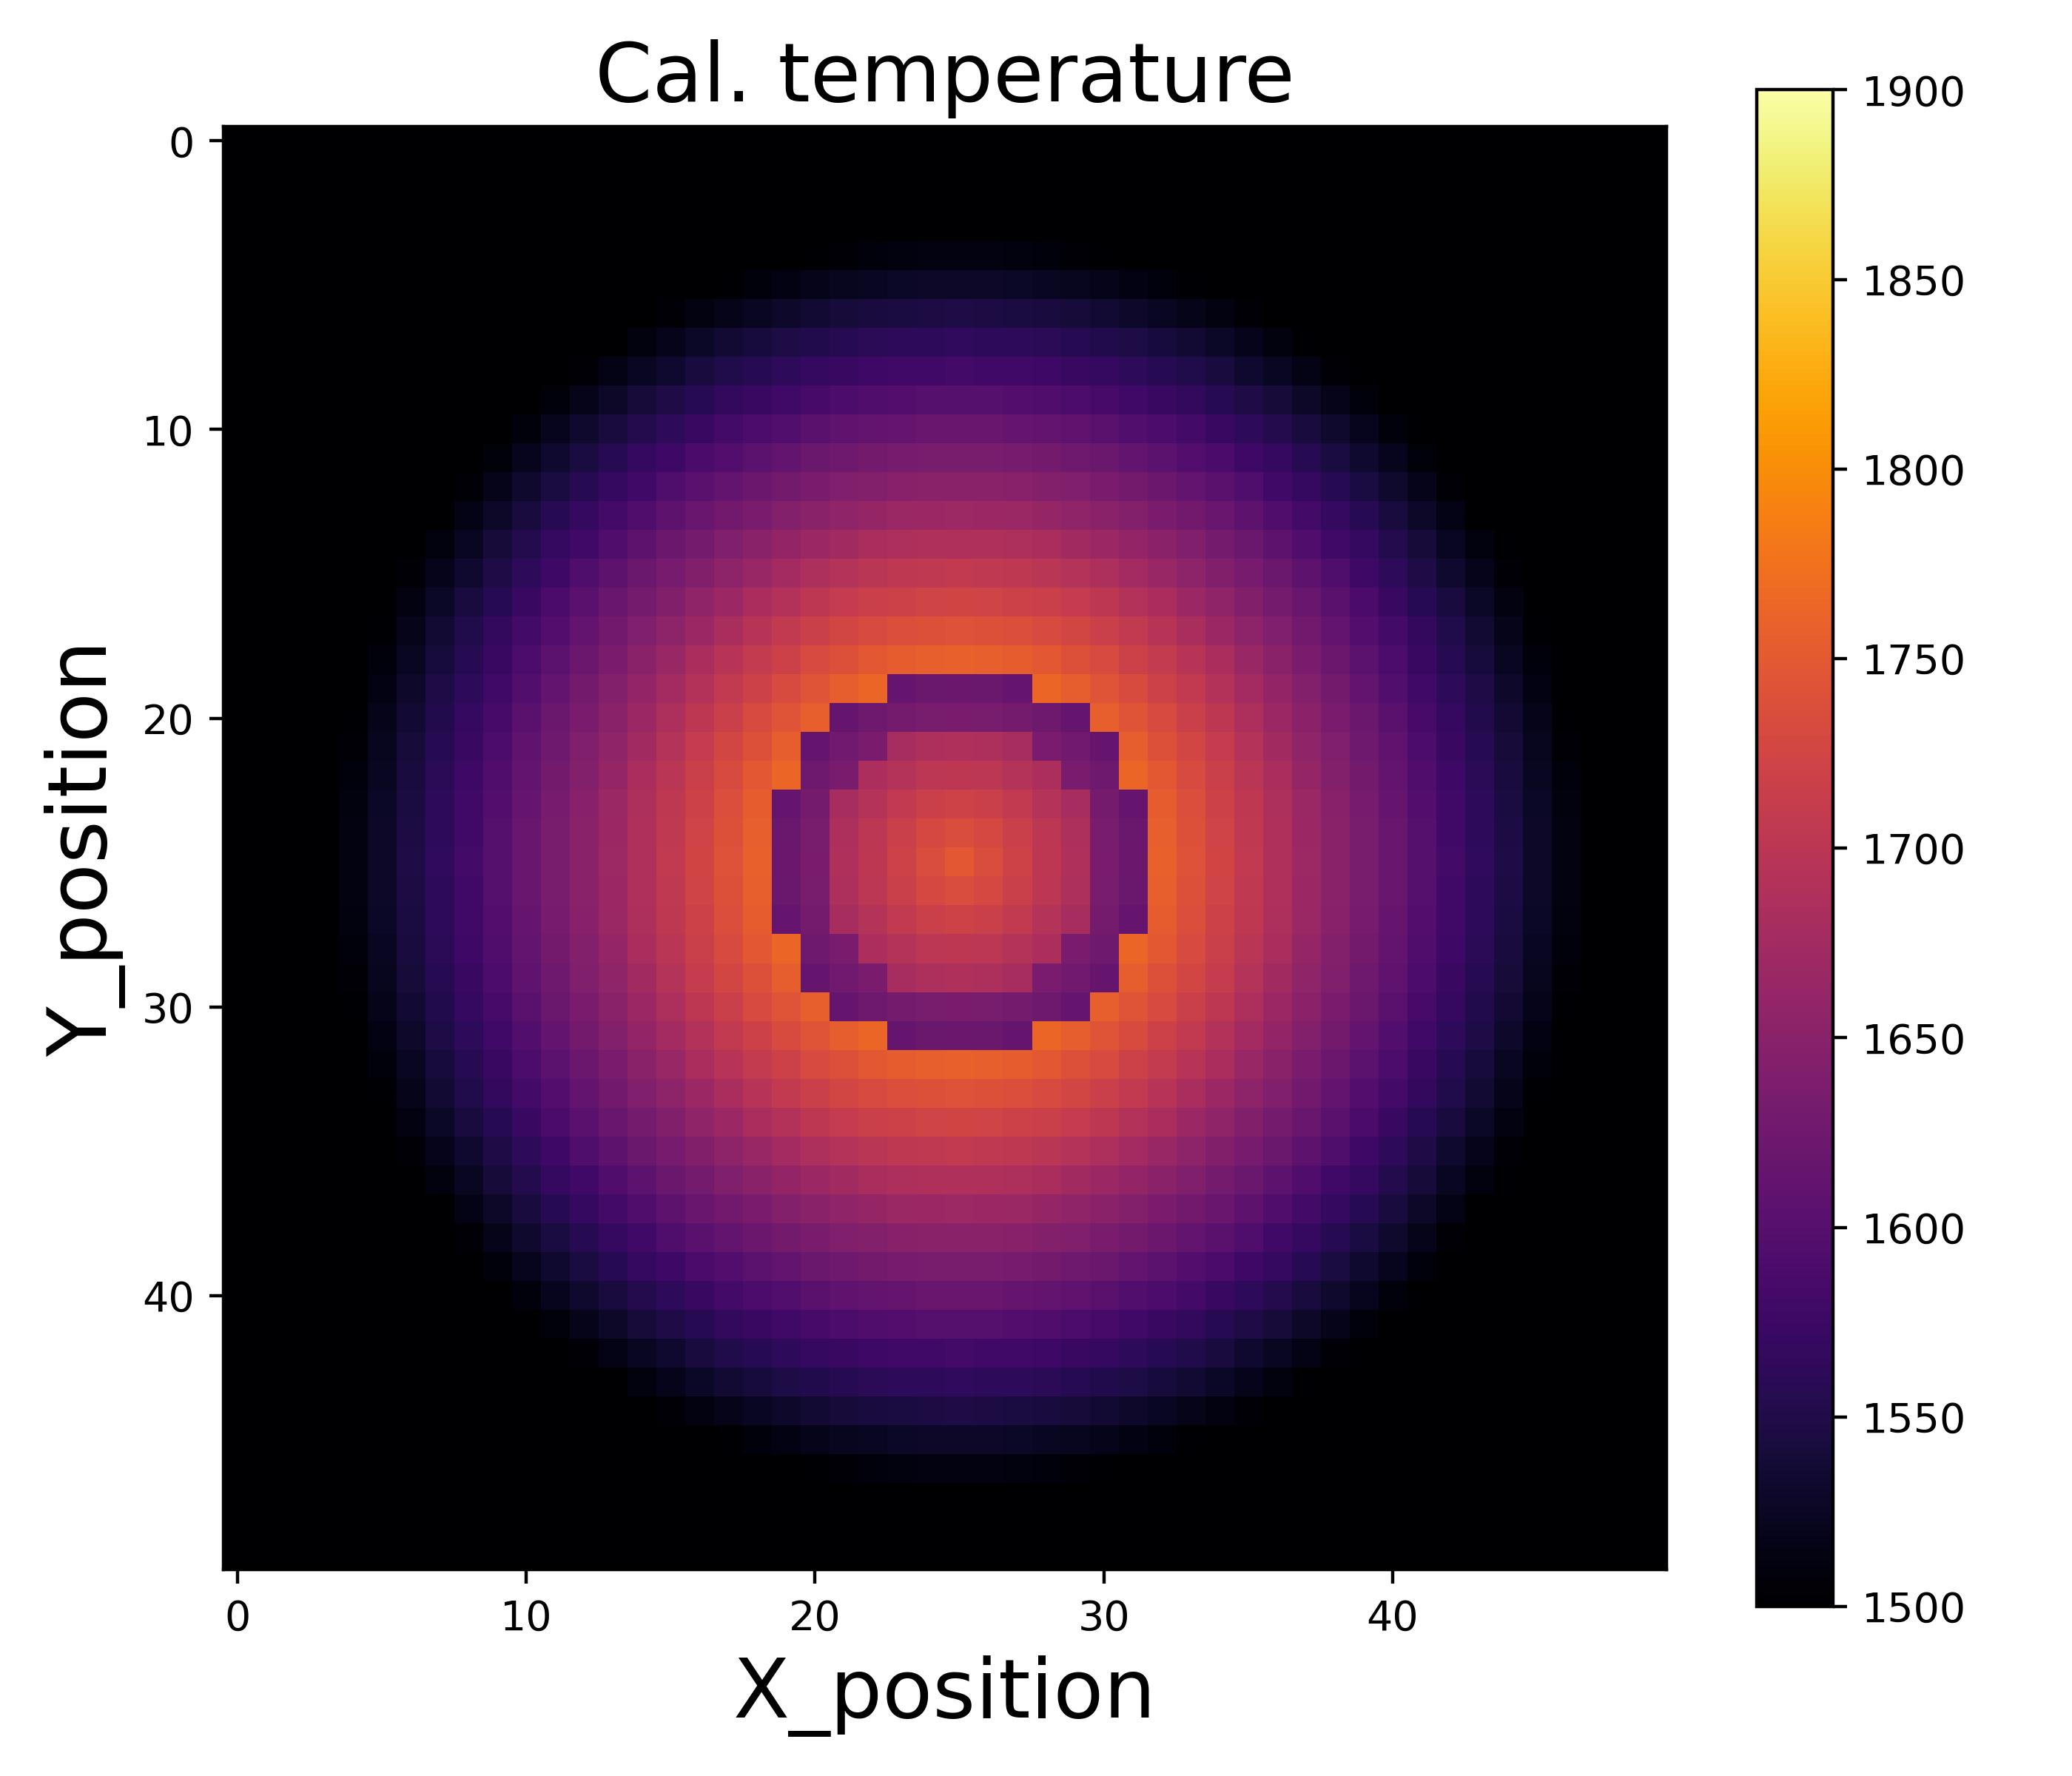
\includegraphics[width=\textwidth]{figures/raw_data/5/mix/T_cal.jpg}
        \end{subfigure}
        \begin{subfigure}{0.325\textwidth}
            \centering
            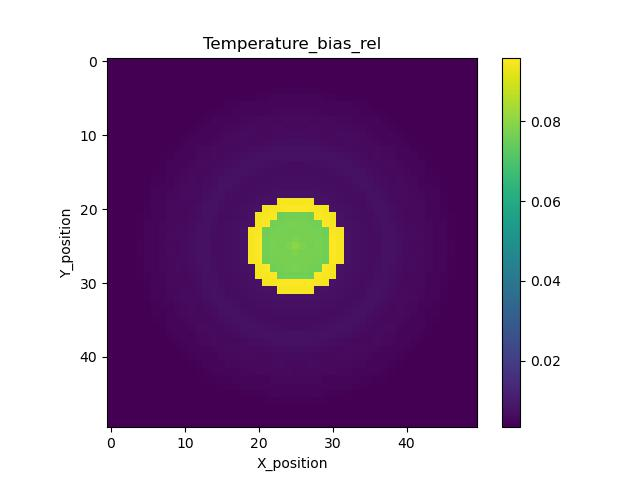
\includegraphics[width=\textwidth]{figures/raw_data/5/mix/T_bias.jpg}
        \end{subfigure}
        \begin{subfigure}{0.325\textwidth}
            \centering
            \includegraphics[width=\textwidth]{figures/raw_data/5/mix/emi_cal.jpg}
        \end{subfigure}
        \subcaption{Material based on real iron data}
    \end{minipage}
    \caption{Calculation results of mixed model}
    \label{fig: result_mixed_model}
\end{figure}


From Fig.\ref{fig: result_mixed_model}, it is evident that the mixed model 
accurately identifies the boundaries between the liquid and solid regions 
for both model 1 based material and real iron-based material. 
Additionally, it accurately recognizes the regions that require 
recalculations in the case of blackbody materials. This indicates that 
the model is applicable to materials with different emissivity characteristics.


Regarding the temperature estimation results, the model demonstrates high 
precision in calculating temperatures for blackbody materials and materials 
based on model 1. In these cases, the error in the center region is less than 7\%. 
However, the model shows a region of relatively lower accuracy when 
applied to real iron-based material. In this region, the emissivity values 
are erroneously computed as 1, leading to an increase in temperature 
calculation bias. This discrepancy can be attributed to the use of the 
exponential model in the temperature estimation algorithm, as mentioned 
earlier, which introduces errors when calculating the emissivity 
of real iron in its liquid state.


\section{Statistical results and analysis}

After obtaining all calculation results, some statistical results can be found in 
tabel \ref{tab: statistic_results}. To mitigate any negative impact of background 
regions on the statistical results of the temperature estimation algorithm, 
only the computation results from the central area of the observation 
area are considered here. As linear temperature distribution 
is employed for the hypothetical materials, temperature is used to determine 
whether the point is within 
the central area. These conditions can be formulated as follows:


\begin{equation}
    P = \begin{cases}
        P_{center}  & T \geq T_{edge} \\
        P_{background}  & T < T_{edge}
    \end{cases}
    \label{eq: T_edge}
\end{equation}


With $T_{edge} = 1200K$ for materials based on model and $T_{edge} = 1600K$ for materials based 
on real iron data. This is due to the fact that in the virtual experimental 
platform, the temperature of the background area in the experiments based on 
real iron data is set to $1500K$.


Table \ref{tab: statistic_results} presents the statistical results of five 
different temperature estimation algorithms: linear model, linear square model, 
quadratic model, exponential model and mixed model. These algorithms were 
applied to blackbody materials, real materials, and materials based on \mbox{Model 1-9}. 
The statistical metrics calculated for each algorithm include:


\begin{enumerate}
    \item Mean Difference(Difference)
    \item Mean Relative Error(Rel. difference)
    \item Standard Deviation(SD)
    \item Maximum Relative Error
    \item Minimum Relative Error
\end{enumerate}

\subsubsection{Mean Difference}
The mean difference describes the difference between the calculated 
temperature $T_{cal}$ and the actual temperature $T_{act}$. It intuitively 
demonstrates the accuracy of the temperature estimation algorithm. It is 
defined by the following equation:

\begin{equation}
    {E} = \overline{T_{cal} - T_{act}} 
\end{equation}

\subsubsection{Mean Relative Error}
The mean relative error describes the relative difference between the calculated 
temperature $T_{cal}$ and the actual temperature $T_{act}$. To avoid mutual 
cancellation between positive and negative deviations, the absolute value of 
the relative deviation is used here. The mathematical equation can be found as follows:

\begin{equation}
    {E}_{rel} = \overline{\left\lvert \frac{T_{cal} - T_{act}}{T_{act}}\right\rvert }
\end{equation}

\subsubsection{Standard Deviation}
The standard deviation is used to describe the distribution of differences 
between the calculated temperature $T_{cal}$ and the actual 
temperature $T_{act}$. Since a linear temperature distribution is used, the 
temperature range of materials within the observed area is relatively large. 
Hence, this standard deviation can be used to characterize the consistency of the 
temperature estimation algorithm's results under different temperature conditions.
The definition can be found by the following equation:

\begin{equation}
    \sigma = \sqrt{\frac{\sum {\left\lvert T_{cal} - T_{act}\right\rvert }^2}{N}} 
\end{equation}

With $N$ represents the number of points involved in the statistical analysis.

\subsubsection{Min. and Max. Relative Error}
These two parameters describe the maximum and minimum values of the relative 
difference between the calculated temperature $T_{cal}$ and the actual temperature 
$T_{act}$ over the entire statistical region. These parameters can be used to 
observe the maximum and minimum errors caused by the temperature estimation 
algorithm. This allows for a visual assessment of the effectiveness boundaries 
of the temperature estimation algorithm's results.



\begin{sidewaystable}[htbp]
    \centering
    \caption{Calculation results from different models}
    \label{tab: statistic_results}
    \begin{tabular}{lccccccccccc}
        \hline
        & \multicolumn{1}{c}{Black body} & \multicolumn{1}{c}{Real data} & Model 1 & Model 2 & Model 3 & Model 4 & Model 5 & Model 6 & Model 7 & Model 8 & Model 9 \\ \hline
        \multicolumn{12}{c}{Linear}                                                                                                                                                         \\ \hline
        Difference {[}K{]}      & 20.7                           & -151.7                        & 129.5   & 38.8    & 58.6    & 116.5   & -4.8    & -39.6   & -161.6  & 445.5   & 27.2     \\
        Rel. difference         & 0.02                           & 0.08                          & 0.08    & 0.03    & 0.04    & 0.08    & 0.02    & 0.04    & 0.11    & 0.32    & 0.02     \\
        SD {[}K{]}              & 7.06                           & 9.56                          & 115.31  & 44.97   & 73.78   & 98.33   & 57.27   & 104.74  & 112.38  & 157.94  & 20.80    \\
        Max. difference {[}K{]} & 0.029                          & 0.096                         & 0.160   & 0.073   & 0.145   & 0.140   & 0.167   & 0.170   & 0.263   & 0.489   & 0.057    \\
        Min. difference {[}K{]} & 0.006                          & 0.076                         & 0.0001  & 0.0004  & 0.0001  & 0.0001  & 0.00    & 0.0001  & 0.001   & 0.031   & 0.0003   \\ \hline
        \multicolumn{12}{c}{Linear square}                                                                                                                                                   \\ \hline
        Difference {[}K{]}      & 38.7                           & 30.8                          & 102.9   & -13.1   & 24.4    & 72.9    & -31.1   & 96.5    & -122.5  & 423.9   & -10.6   \\
        Rel. difference         & 0.03                           & 0.02                          & 0.07    & 0.03    & 0.03    & 0.05    & 0.02    & 0.07    & 0.08    & 0.30    & 0.03    \\
        SD {[}K{]}              & 23.95                          & 6.88                          & 8.21    & 42.45   & 36.18   & 11.12   & 57.39   & 27.09   & 45.99   & 93.41   & 58.86   \\
        Max. difference {[}K{]} & 0.074                          & 0.079                         & 0.105   & 0.059   & 0.071   & 0.088   & 0.101   & 0.115   & 0.118   & 0.379   & 0.093   \\
        Min. difference {[}K{]} & 0.006                          & 0.013                         & 0.03    & 0.000   & 0.0001  & 0.031   & 0.0001  & 0.011   & 0.018   & 0.03    & 0.0001  \\ \hline
        \multicolumn{12}{c}{Quadratic}                                                                                                                                                 \\ \hline
        Difference {[}K{]}      & 19.3                           & -151.7                        & 104.7   & 41.5    & 8.6     & 88.1    & 76.7    & -47.8   & -212.7  & 509.9   & 113.1   \\
        Rel. difference         & 0.01                           & 0.09                          & 0.09    & 0.09    & 0.04    & 0.10    & 0.11    & 0.03    & 0.14    & 0.37    & 0.12    \\
        SD {[}K{]}              & 4.07                           & 9.56                          & 194.96  & 214.93  & 144.50  & 216.52  & 239.63  & 96.18   & 117.62  & 167.72  & 234.07  \\
        Max. difference {[}K{]} & 0.022                          & 0.096                         & 0.336   & 0.329   & 0.280   & 0.352   & 0.321   & 0.166   & 0.280   & 0.630   & 0.341   \\
        Min. difference {[}K{]} & 0.006                          & 0.076                         & 0.005   & 0.003   & 0.000   & 0.005   & 0.0003  & 0.0001  & 0.092   & 0.031   & 0.003   \\ \hline
        \multicolumn{12}{c}{Exponential}                                                                                                                                                   \\ \hline
        Difference {[}K{]}      & 20.5                           & -147.3                        & 102.9   & -12.9   & 24.4    & 72.9    & -60.5   & 96.6    & -406.4  & 318.2   & -91.6   \\
        Rel. difference         & 0.01                           & 0.08                          & 0.07    & 0.03    & 0.03    & 0.05    & 0.04    & 0.07    & 0.45    & 0.325   & 0.235    \\
        SD {[}K{]}              & 16.70                          & 24.63                         & 8.23    & 42.15   & 36.19   & 11.14   & 56.69   & 27.04   & 523.51  & 385.45  & 343.71  \\
        Max. difference {[}K{]} & 0.075                          & 0.096                         & 0.105   & 0.056   & 0.071   & 0.088   & 0.101   & 0.115   & 0.644   & 0.630   & 0.452   \\
        Min. difference {[}K{]} & 0.006                          & 0.013                         & 0.031   & 0.00    & 0.0001  & 0.03    & 0.0005  & 0.012   & 0.031   & 0.002   & 0.003   \\ \hline
        \multicolumn{12}{c}{Mixed model}                                                                                                                                                   \\ \hline
        Difference {[}K{]}      & 14.6                           & -34.6                         & 102.9   & -12.9   & 24.4    & 72.9    & -31.1   & 96.6    & -122.5  & 424.16  & -10.6    \\
        Rel. difference         & 0.01                           & 0.02                          & 0.07    & 0.03    & 0.03    & 0.05    & 0.02    & 0.07    & 0.08    & 0.30    & 0.025    \\
        SD {[}K{]}              & 6.17                           & 53.49                         & 8.22    & 42.14   & 36.19   & 11.13   & 57.39   & 27.04   & 45.98   & 93.88   & 85.86  \\
        Max. difference {[}K{]} & 0.017                          & 0.096                         & 0.105   & 0.056   & 0.071   & 0.088   & 0.101   & 0.115   & 0.118   & 0.382   & 0.093   \\
        Min. difference {[}K{]} & 0.00                           & 0.006                         & 0.03    & 0.000   & 0.0001  & 0.031   & 0.000   & 0.012   & 0.018   & 0.031   & 0.0001  
    \end{tabular}
\end{sidewaystable}


\subsection{Performance of different temperature estimation algorithms}
After obtaining the statistical results of the temperature estimation algorithm, 
it is necessary to analyze these results. Since the statistical outcomes 
encompass the calculations of various temperature estimation algorithms 
for different materials, the analysis consists of two main parts: one involves 
the performance analysis of different temperature estimation algorithms, 
while the other concerns the performance analysis of the temperature estimation 
algorithm for different materials.


In Table \ref{tab: statistic_results}, it can be observed that each temperature 
estimation algorithm produces different results for the same material. 


When applied to blackbody materials, all algorithms achieve accuracy
within 5\% error. However, it is evident that the linear square model 
exhibits lower precision compared to other models, and simultaneously, 
the standard deviation of its calculations is significantly higher than 
that of other temperature estimation algorithms. This discrepancy could be 
attributed to the linear square model having an additional parameter, which 
makes the curve-fitting process more prone to encountering local minima and 
prematurely terminating the computation.


Indeed, in addition to linear square model's performance on blackbody materials, the temperature 
estimation algorithm based on the linear square model consistently achieves 
lower relative errors and standard deviations compared to other temperature 
estimation algorithms when applied to different materials. This indicates that 
the linear square model not only attains higher accuracy but also exhibits a 
higher level of computation consistency.


In contrast to the linear square model, the temperature estimation algorithm 
based on the quadratic model exhibits lower consistency in computing results 
for hypothetical materials in this work. The standard deviation for this 
metric is close to or exceeds 100K. This indicates that the temperature 
estimation algorithm based on the quadratic model cannot demonstrate 
high consistency in the calculations of the virtual materials used in this 
work. This is attributed to the emissivity characteristics of the hypothetical materials 
used in this study, which do not conform well to the profile of the quadratic 
function. Consequently, the curve fit algorithm fails to find stable global 
optimal points, resulting in lower consistency in the computed results.


The temperature estimation algorithm based on the exponential model demonstrates 
comparable accuracy and consistency to the temperature estimation algorithm 
based on the linear square model when applied to blackbody material
and materials based on model 1, 2, 3, 4, and 6. Furthermore, it offers 
significant time savings in computational efforts. In situations where the 
emissivity variation is limited, this model exhibits a higher propensity to 
yield stable local optima, making it particularly suitable for application 
in the liquid phase region of hypothetical materials based on models.


It is evident from the results that different temperature estimation algorithms 
exhibit varying performance when applied to experimental data from different 
materials. To address this, the author proposes utilizing a temperature estimation 
algorithm based on the mixed model to effectively combine the advantages of 
different estimation approaches, especially for materials with complex emissivity 
characteristics. Table \ref{tab: statistic_results} illustrates that the mixed 
model outperforms the linear square model and exponential model in the 
computation of blackbody materials, showing better accuracy and consistency. 
Moreover, across all other models, the temperature estimation algorithm based 
on the mixed model consistently yields the better result in the two 
original temperature estimation algorithms.

\subsection{Performance of temperature estimation algorithm between different materials}

\begin{figure}[htbp]
    \centering
    \begin{subfigure}{\textwidth}
        \includegraphics[width=\textwidth]{figures/diff_rel.jpg}
        \subcaption{Mean relative error}
    \end{subfigure}\\
    \begin{subfigure}{\textwidth}
        \includegraphics[width=\textwidth]{figures/diff_std.jpg}
        \subcaption{Standard deviation}
    \end{subfigure}
    \caption{Mean relative error and standard deviation of calculation results}
    \label{fig: result_final_analysis}
\end{figure}

Fig.\ref{fig: result_final_analysis} presents the computational results of 
temperature estimation using five different temperature estimation algorithms 
on various hypothetical materials. 


In temperature estimation for blackbody materials, all emissivity models yield accurate 
results with acceptable consistency. This phenomenon arises from the fact that 
the emissivity of blackbody materials remains constant regardless of wavelength.
This characteristic allows the avoidance of emissivity's impact on the estimated 
temperature during the curve fitting process, thus enhancing both the accuracy 
and consistency of the calculations.


In the calculation of hypothetical material based on real iron data, 
the temperature estimation algorithms based on the linear square model and the 
mixed model exhibit mean relative errors below 5\%. Other models also achieve 
mean relative errors below 10\%. Concerning computational consistency, 
apart from the mixed model and exponential model, the standard deviations of the 
remaining models are within 10K, while the mixed model and exponential model have 
standard deviations exceeding 20K. This phenomenon is attributed to the exponential 
model's inability to adequately 
fit the emissivity behavior within the liquid phase region of real iron data. 
Consequently, this inadequacy leads to a decrease in the accuracy of temperature 
estimation. Meanwhile, it is noteworthy that the temperature estimation algorithm 
based on the mixed model alters the emissivity model during its operation, thereby 
resulting in a reduction in the consistency of the computed results.


In contrast to the first two materials, for materials based on model 1, 2, 3, 4, 5, 
6, and 9, the mixed model and linear square model exhibit similar performance 
in temperature estimations. Both models are capable of achieving a mean relative 
error in temperature estimation of less than 10\%. On the other hand, the quadratic 
model demonstrates relatively inferior performance. Its computational result 
exhibit both higher mean relative error and lower consistency in calculations. 
This observation suggests that the temperature estimation algorithm based on the 
quadratic model is not suitable for calculating temperatures of the hypothetical 
materials mentioned in this work. Conversely, the temperature estimation algorithms 
based on the linear square model and the mixed model can achieve higher precision 
in temperature estimation for these hypothetical materials.


For models 7 and 8, all temperature estimation algorithms exhibit lower 
computational accuracy and consistency. Particularly in model 8, 
none of the five temperature estimation algorithms are capable of providing 
effective temperature estimation results. This issue arises from the inability 
of these algorithms to fit the emissivity behavior of model 8, leading to 
ineffective temperature estimation results. Consequently, it is evident that the 
emissivity model plays a crucial role in temperature estimation algorithms, 
serving as a key determinant of their accuracy and consistency.


\section{System limitations and boundaries}
In the aforementioned analysis, it can be observed that the virtual 
experimentation platform, along with the temperature estimation system, 
are not devoid of imperfections. During utilization, they also exhibit 
certain limitations and systemic boundaries.


\subsection{Raw material data in virtual experiment platform}
As mentioned earlier, the emissivity of the hypothetical materials used in the virtual experiment 
platform is primarily determined by two terms. The first term is wavelength related, while the 
second term temperature related. It follows that when the virtual experiment platform generates 
experimental data, the parameters of the experiment (such as the hypothetical material's 
temperature and the wavelength range of the virtual multispectralmeter) need to fall within the 
range of the original dataset. Although the extrapolation method was employed in the work to prevent 
computational errors, this practice still contributes to a reduction in the reality 
of the generated experimental data.

\subsection{Performance of temperature estimation algorithm at high target temperature}

\subsection{Emissivity model in temperature estimation algorithm}